\documentclass[a4paper,10pt]{book}
%\documentclass[a4paper,10pt]{article}
\usepackage[utf8]{inputenc}
\usepackage[spanish]{babel}
%\usepackage{showkeys}
\usepackage{bbm}
\usepackage[margin=2.5cm]{geometry}
\usepackage{amsmath,amssymb}
\usepackage{bigints}
\usepackage{enumerate} 
\usepackage{setspace}
\usepackage{hyperref}
\usepackage{listings,color}
\usepackage{graphicx}
\hypersetup{
    %bookmarks=true,         % show bookmarks bar?
    unicode=false,          % non-Latin characters in Acrobat’s bookmarks
    pdftoolbar=true,        % show Acrobat’s toolbar?
    pdfmenubar=true,        % show Acrobat’s menu?
    pdffitwindow=false,     % window fit to page when opened
    pdfstartview={FitH},    % fits the width of the page to the window
    pdftitle={Problema del TC},    % title
    pdfauthor={Ivan Mandelman},     % author
    pdfsubject={Tesis de Lic. en Matematica},   % subject of the document
    pdfcreator={Ivan Mandelman},   % creator of the document
    pdfproducer={Ivan Mandelman}, % producer of the document
    pdfkeywords={Tesis} {Optimizacion} {TC}, % list of keywords
    pdfnewwindow=true,      % links in new window
    colorlinks=true,       % false: boxed links; true: colored links
    linkcolor=red,          % color of internal links
    citecolor=green,        % color of links to bibliography
    filecolor=magenta,      % color of file links
    urlcolor=blue           % color of external links (cyan)
}

\definecolor{mygreen}{rgb}{0,0.6,0}
\definecolor{mygray}{rgb}{0.5,0.5,0.5}
\definecolor{mymauve}{rgb}{0.58,0,0.82}

\lstset{ %
  backgroundcolor=\color{white},   % choose the background color; you must add \usepackage{color} or \usepackage{xcolor}
  basicstyle=\footnotesize,        % the size of the fonts that are used for the code
  breakatwhitespace=false,         % sets if automatic breaks should only happen at whitespace
  breaklines=true,                 % sets automatic line breaking
  captionpos=b,                    % sets the caption-position to bottom
  commentstyle=\color{mygreen},    % comment style
  deletekeywords={...},            % if you want to delete keywords from the given language
  escapeinside={\%*}{*)},          % if you want to add LaTeX within your code
  extendedchars=true,              % lets you use non-ASCII characters; for 8-bits encodings only, does not work with UTF-8
  frame=single,	                   % adds a frame around the code
  keepspaces=true,                 % keeps spaces in text, useful for keeping indentation of code (possibly needs columns=flexible)
  keywordstyle=\color{blue},       % keyword style
  language=Octave,                 % the language of the code
  otherkeywords={*,...},           % if you want to add more keywords to the set
  numbers=none,                    % where to put the line-numbers; possible values are (none, left, right)
  numbersep=5pt,                   % how far the line-numbers are from the code
  numberstyle=\tiny\color{mygray}, % the style that is used for the line-numbers
  rulecolor=\color{black},         % if not set, the frame-color may be changed on line-breaks within not-black text (e.g. comments (green here))
  showspaces=false,                % show spaces everywhere adding particular underscores; it overrides 'showstringspaces'
  showstringspaces=false,          % underline spaces within strings only
  showtabs=false,                  % show tabs within strings adding particular underscores
  stepnumber=2,                    % the step between two line-numbers. If it's 1, each line will be numbered
  stringstyle=\color{mymauve},     % string literal style
  tabsize=2,	                   % sets default tabsize to 2 spaces
%  title=\lstname                   % show the filename of files included with \lstinputlisting; also try caption instead of title
}
%\newcommand{\xcal}[1]{\text{\usefont{OMS}{cmsy}{m}{n}#1}}
%\DeclareMathAlphabet{\mathpzc}{OMS}{cmex}{m}{n}
\DeclareMathAlphabet{\mathpzc}{OT1}{pzc}{m}{n}
%\DeclareMathAlphabet{\mathcalligra}{T1}{calligra}{m}{n}
%\newcommand{\mycal}{\usefont{OT1}{pzc}{m}{n}\fontsize{10}{12}\selectfont} 

\newcommand{\N}{\mathbbm{N}}
\newcommand{\R}{\mathbbm{R}}
\newcommand{\Rn}{\R^n}
\newcommand{\arr}{\rightarrow}
\newcommand{\bx}{\bar{x}}
\newcommand{\blambda}{\bar{\lambda}}
\newcommand{\bmu}{\bar{\mu}}
\newcommand{\cN}{\mathcal{N}}
\newcommand{\cT}{\mathcal{T}}
\newcommand{\cI}{\mathpzc{I}}
\newcommand{\cE}{\mathpzc{E}}
\newcommand{\cA}{\mathpzc{A}}
\newcommand{\la}{\langle}
\newcommand{\ra}{\rangle}
\newcommand{\deb}{\rightharpoonup}

\newtheorem{teo}{Teorema}%[section]
\newtheorem{lem}[teo]{Lema}
\newtheorem{cor}[teo]{Corolario}
\newtheorem{prop}[teo]{Proposici\'on}
\newtheorem{defi}[teo]{Definici\'on}
%\newtheorem{defi}{Definici\'on}[chapter]
%\newtheorem{ejem}[teo]{Ejemplo}
\newcounter{ejem}[section]
\newenvironment{ejem}[1][]{\refstepcounter{ejem}\par\medskip
   \noindent \textbf{Ejemplo~\theejem. #1} \rmfamily}{\medskip}
\newenvironment{dem}{\vspace*{-0.1cm}{\it Demostraci\'on:}}{\hfill
$\blacksquare$\\} 

%\title{Trayectorias de tiempo óptimo \\para circuitos cerrados}
%\author{\vspace{5.4cm}\\ \hspace{3.6cm} Autor: Iván Mandelman\\ \hspace{4.3cm} Director: Dami\'an Fern\'andez}
%\date{diciembre de 2017}



% \begin{figure}
% \centering
% \href{http://creativecommons.org/licenses/by-sa/4.0/}{
\includegraphics{Licencia/licencia.png}}
% \caption{\href{http://creativecommons.org/licenses/by-sa/4.0/}{Trayectorias de tiempo óptimo para circuitos cerrados por Iván Mandelman, Damián Fernández se distribuye bajo una}}
% \end{figure}



\begin{document}
%\maketitle
\begin{titlepage}
	\centering
	{\scshape Universidad Nacional de Córdoba \\ Facultad de Matemática, Astronomía, Física y Computación}\\
	
\includegraphics[scale=0.1]{graficos/UNC_escudo}\par\vspace{1cm}
	{\scshape\Large Trabajo Especial de Grado\par}
%	\vspace{1cm}
	{\huge\bfseries Trayectorias de tiempo óptimo \\para circuitos cerrados\par}
	\vspace{1cm}
	Autor: Iván Mandelman\\  Director: Dami\'an Fern\'andez \\  4 de diciembre de 2017
% 	\begin{tabular}{p{0.5\textwidth} l}
% 	& Autor: Iván Mandelman\\ & Director: Dami\'an Fern\'andez \\ & 4 de diciembre de 2017
% 	\end{tabular}
%	\vspace{5cm}




	\vfill
	\begin{tabular}{rp{0.75\textwidth}}
	\href{http://creativecommons.org/licenses/by-sa/4.0/}{
\includegraphics[scale=0.5]{Licencia/licencia.png}} & \vspace{-0.8cm}
	Trayectorias de tiempo óptimo para circuitos cerrados por Iván Mandelman y Damián Fernández se distribuye bajo una
	\href{http://creativecommons.org/licenses/by-sa/4.0/}{Licencia Creative Commons Atribución-CompartirIgual 4.0 Internacional}
	\end{tabular}

\end{titlepage}



\section*{Resumen}
    Las trayectorias de tiempo óptimo en circuitos cerrados son usadas, por ejemplo, para determinar el camino que debe seguir un vehículo en una carrera o el recorrido de un riel en una línea de producción. Desde el punto de vista matemático, se plantea un problema de minimización de un cierto funcional (representante del tiempo) en el espacio de las curvas cerradas y sujeto a condiciones propias del problema.
    
    El objetivo de este trabajo es el de analizar y resolver el problema de optimización de encontrar una trayectoria óptima para un circuito cerrado, de manera que minimice el tiempo que se demora en recorrerlo. En el problema a analizar se planteará un modelo que contemple ciertas restricciones de permanencia en el circuito y fricción correspondientes.
    
    Además en este trabajo se analizará el problema a resolver para lograr modelarlo matemáticamente. Luego se darán las herramientas teóricas y técnicas numéricas para resolver el problema. Con el modelo matemático listo, se procederá a realizar una discretización del problema para resolverlo computacionalmente y finalmente se exhibirán los resultados numéricos obtenidos con su interpretación gráfica correspondiente.
    
\vfill
\paragraph{Palabras Claves:} trayectorias en circuitos cerrados, optimización no lineal.
\paragraph{Clasificación (MSC2010):}
\begin{itemize}
   \item[90C90] Operations research, mathematical programming. Applications of mathematical programming.
   \item[65D17] Numerical analysis. Computer aided design (modeling of curves and surfaces).
\end{itemize}
\newpage

\section*{Abstract}
   Optimal time trajectories in closed tracks are used, for example, to determine the path that a vehicle must follow in a race or the route of conveyor system in an assembly line.
   From a mathematical point of view a minimization problem is set in the space of closed curves subject to conditions that are problem related.
   
    The objective of this work is to analyze and solve the optimization problem of finding an optimal trajectory for a closed track, so that minimize the time that is taken to go over the track. In this problem it will be set a model that contemplates some constraints like staying inside the track and satisfying a friction equation.
    
    In addition, in this work the problem will be analyzed to achieve a mathematical model. Then theoretical tools and numerical techniques will be given to solve the problem. When the mathematical model is finished, it will be performed a discretization to computationally solve the problem and finally, numerical results will be exhibited and a respective graphic interpretation given. 

\vfill
\paragraph{Palabras Claves:} trajectories in closed tracks, nonlinear programming.
\paragraph{Clasificación (MSC2010):}
\begin{itemize}
   \item[90C90] Operations research, mathematical programming. Applications of mathematical programming.
   \item[65D17] Numerical analysis. Computer aided design (modeling of curves and surfaces).
\end{itemize}

    
    

\tableofcontents

\pagebreak

\section*{Notaci\'on}
{\setlength{\parindent}{0cm}
%{\setstretch{1.5}
$:=$ igual por definición.

$\emptyset$ conjunto vacío.

\hangindent=1cm \textbf{p.p.} para casi todo punto, es decir, en todos los puntos excepto posiblemente en los de medida (medida dada por el contexto) cero.

$x\to f(x)$ mapea el punto $x$ hacia $f(x)$.

$F:X\arr Y$ la función $F$ sale del espacio $X$ y llega al espacio $Y$.

$\R$ los números reales.

$\Rn$ es el espacio euclídeo $n$-dimensional.

$\Rn_+=\{x\in\Rn\,|\,x_i\geq0,\,i=1,\ldots,n\}$ es el ortante no negativo.

\hangindent=1cm $L_2[0,1]$ el espacio de Hilbert de clases de equivalencias de valores reales, cuadrado integrable, funciones $\psi(t)$, con $\psi_1\sim\psi_2$ si $\psi_1(t)=\psi_2(t)$ para todo $t\in[0,1]$ excepto posiblemente en un conjunto de medida Lebesgue cero, y $\la\psi,\varphi\ra=\int_0^1\psi(t)\varphi(t)dt$.

\hangindent=1cm $L_p(\Omega)$ espacio de Banach de funciones medibles Lebesgue $\psi\!:\!\Omega\arr\R$ con norma finita $\|\psi\|_p\!:=\!(\int_{\Omega}\!|\psi(\omega)|^p d\omega)^{\frac{1}{p}}$.

$L_p(\Omega)_+\subset L_p(\Omega)$ el conjunto de funciones con valores no negativos p.p. $x\in\Omega$.

\hangindent=1cm $W^{m,s}(\Omega)=\{\psi\in L_s(\Omega)\,|\, D^q\psi\in L_s(\Omega)\mbox{ si }|q|\leq m\}$ espacio de Sobolev, donde $D^q\psi=\frac{\partial^{|q|}\psi}{\partial_{x_1}^{q_1}\ldots\partial_{x_l}^{q_l}}$ y $|q|=q_1+\ldots+q_l$.

$H^m(\Omega)$ es el espacio de Sobolev $W^{m,2}(\Omega)$.

$C_c^\infty(\Omega)$ son las funciones infinitamente diferenciables de soporte compacto.

\hangindent=1cm $\mathcal{L}(X,Y)$ espacio de operadores lineales continuos $A:X\arr Y$ con la norma $\|A\|=\sup_{\|x\|<1}\|Ax\|$ siendo $X$ e $Y$ espacios normados.

$X^*=\mathcal{L}(X,\R)$ espacio dual de $X$.

$\mbox{span}\{S\}$ es el subespacio generado por el conjunto $S\subset X$ donde $X$ es un espacio vectorial.

int($S)=\{x\in S\,|\, \exists\mbox{ un entorno }V \mbox{ de }x\mbox{ tal que }V\subset S\}$ es  el interior del conjunto $S$.

$r(t)=o(t)$ si $r:\R_+\to\R$ cumple que $r(t)/t\to 0$ cuando $t\to0$.

$\varliminf_{n\to\infty}x_n=\sup_{n\geq0}\mbox{inf}_{k\geq n}(x_k)$ es el límite inferior de una sucesión $\{x_n\}$.

$\varlimsup_{n\to\infty}x_n=\mbox{inf}_{n\geq 0}\sup_{k\geq n}(x_k)$ es el límite superior de una sucesión $\{x_n\}$.

$\mbox{cl}(S)$ es la clausura (con la topología usual) del conjunto $S$.

Si $A$ y $B$ son espacios vectoriales, $A+B=\{a+b\mid a\in A,\, b\in B\}$ es la suma de Minkowski.

$A^t$ es la transpuesta de la matriz $A$.


$A(:,m:l)$ son todas las filas, y las columnas desde la $m$ hasta la $l$ de la matriz $A$.

$[A;B]$ es una matriz formada por el bloque $A$ y en la fila debajo, el bloque $B$.

$B(a,\varepsilon)=\{x\in\Rn\mid \|x-a\|_{\Rn}<\varepsilon\}$ es la bola abierta de $\Rn$.

$B[a,\varepsilon]=\{x\in\Rn\mid \|x-a\|_{\Rn}\leq\varepsilon\}$ es la bola cerrada de $\Rn$.

$\mathrm{Im}(f)$ es la imagen de la función $f$. 

\hangindent=1cm En el caso en que el contexto no lo especifique, la derivada de una función en un punto $x$, $f'(x)$ con $f:\Rn\arr\R$, será considerada como una matriz de $n$ filas y $1$ columna. De la misma manera, consideraremos un vector en $\Rn$ como un vector columna.

Si no se aclara lo contrario $\{x_k\},\, k\in\N$ denotara la sucesión de números reales $x_1,x_2,\ldots$

$C^l(\Omega)$ es el espacio de Banach de funciones $\psi:\Omega\arr\R,\ \Omega\in\Rn$ $l$-veces continuamente diferenciables. 

Si $A:X\arr Y$ es un operador lineal, $\mathrm{Ker}(A)=\{x\in X\mid Ax=0\}$ es el núcleo de $A$.

Si $b,d\in\Rn$, $b\leq d$ significa $b_i\leq d_i,\,\forall i=1,\ldots,n$.

%poner toda la notacion
}

\chapter*{Introducción}

El objetivo de este trabajo es, dado un circuito cerrado con sus respectivos coeficientes de fricción, encontrar la trayectoria que demora menos tiempo en recorrerlo, lo cual se puede traducir en resolver un problema de optimización con restricciones.

En el Capítulo 1, se describe el problema que se desea resolver y se realiza una formulación matemática del mismo, así se obtiene un problema de optimización con restricciones y es posible utilizar marco teórico matemático para resolverlo. Este marco teórico se da a continuación en los siguientes capítulos, en el Capítulo 2 se verán preliminares sobre geometría diferencial, en el Capítulo 3 preliminares de optimización, y en el Capítulo 4, preliminares sobre métodos numéricos. De esta forma, se termina de formular el problema de optimización en el Capítulo 5, cuya idea es obtener un problema como el siguiente

\begin{equation*}
\begin{array}{rl}
\displaystyle \mathop{\mathrm{minimizar}}_{x} & \displaystyle f(x) \\
\mathrm{sujeto \ a} & G(x)\in K,\, x\in C
\end{array}
\end{equation*}
donde se detallan cuáles son los espacios y funciones constituyentes del problema.

Luego, en el capítulo 6, se podrán observar los resultados computacionales de lo planteado anteriormente incluyendo gráficas descriptivas que muestran las trayectorias solución obtenidas.

%explicar el motivo de la tesis con palabras (sin formulas)


\chapter{La trayectoria óptima}

\section{El ``Problema del TC''}
Una manera simple de visualizar el problema que se quiere resolver en este trabajo, es  imaginar encontrarse en alguno de los circuitos del TC (turismo carretera), estos circuitos (o pistas), tienen un punto (o línea) de salida, que es el mismo que el de llegada, y el objetivo, es dar una determinada cantidad de ``vueltas'' en el menor tiempo posible. Resulta muy útil entonces, encontrar una estrategia óptima para \emph{una} vuelta de referencia, considerando que el vehículo comienza a moverse con una velocidad positiva y también termina la vuelta con una velocidad positiva.

Suponer que el vehículo utilizado para recorrer el circuito es un auto, es una restricción que no se contemplará en este trabajo, por lo que se propone un movimiento ``puntual''.

Además, hay otras consideraciones a tener en cuenta:
\begin{itemize}
 \item mantenerse dentro de la pista, esto es indispensable pues se plantea que el terreno fuera de la pista es infranqueable en muchos casos.

 \item la fricción de la pista, que regula los límites de la aceleración, y también, la trayectoria.
\end{itemize}
Por lo tanto la idea es minimizar el tiempo en que se da la vuelta, teniendo en cuenta las consideraciones previas.
Para resolver esto, se plantea un problema de minimización, con determinadas restricciones. La función a minimizar es el tiempo, y algunas de las restricciones deberán ser la permanencia en pista y la fricción.
%\section{formulacion matematica}
\section{Formulación matemática}
%\chapter{preliminares de optimizacion}
%\section{dim infinita}
%% finalizar planteando el problema en este contexto definiendo las funciones y sus derivadas
%\section{discretizacion y dim finita}
%% primero en abstracto y luego
%%discretizacion de los espacios del problema y de las funciones (y derivadas)
%\chapter{resolucion numerica}
%\section{metodo computacional}
%\section{resultado numerico}

El objetivo ahora es definir la función \textbf{tiempo final} $t_f$ que se quiere minimizar, sujeta a las dos condiciones mencionadas anteriormente. Matem\'aticamente la condici\'on de mantenerse dentro de la pista puede escribirse como
\[
x(t)\in \mathcal{P}, \quad\forall t\in[0,t_f],
\]
donde $x$ es la trayectoria del vehículo y $\mathcal{P}$ es el conjunto de curvas que se mantienen dentro de la pista. La condici\'on de fricción regula las aceleraciones tangencial $a_t$ y normal $a_n$ para que cumplan
\begin{equation}\label{elipse}
 \left(\frac{a_t}{\mu_t}\right)^2+ \left(\frac{a_n}{\mu_n}\right)^2\leq g^2, 
\end{equation}
donde $g$ es la aceleración de la gravedad, $\mu_t$ y $\mu_n$ son los coeficientes de rozamiento tangencial y normal, respectivamente. Tal condici\'on es conocida en la literatura como \textbf{elipse de fricción} (ver \cite{rucco2012computing}).

Para estudiar este problema, se definirá la curva $x$ a través de sus funciones de movimiento. Una herramienta que facilitará las cuentas es reparametrizar la curva por longitud de arco.
Entonces se considera la función \textbf{trayectoria} de la curva como $x:[0,t_f]\mapsto \R^2$ tal que
\begin{equation}\label{trayectoria}
x(t) = p c(S(t)), 
\end{equation}
donde \(t_f\) es el tiempo final, $c:[0,1]\arr\R^2$ es una curva parametrizada por longitud de arco, es decir, para $s\mapsto c(s)$ con $s\in[0,1]$
\begin{equation}\label{pla}
\left \|\frac{dc}{ds}(s)\right\|_{\R^2}=1,    
\end{equation}
la funci\'on $S:[0,t_f]\arr [0,1]$ es la longitud de arco normalizada y $p\in(0,+\infty)$ es la longitud de $x$, pues
\[
 \int_0^{t_f} \left\|\frac{dx}{dt}(t)\right\|_{\R^2} dt = p \int_0^{t_f} \frac{dS}{dt}(t)dt=p(S(t_f)-S(0))=p.
\]


Para definir la funci\'on $t_f$ se usarán las propiedades de las funciones anteriormente dadas. Para ello se define la función \textbf{velocidad} $\nu:[0,t_f]\arr\R^2$ tal que
\begin{equation}
  \nu(t)=\frac{dx}{dt}(t)=p\frac{dc}{ds}(S(t))\frac{dS}{dt}(t), \label{velocidad}
\end{equation}
y la funci\'on rapidez (magnitud de la velocidad) $\tilde{v}:[0,t_f]\arr\R_+$ tal que
\[
 \tilde{v}(t)=p\frac{dS}{dt}(t).
\]
Note que estas funciones están definidas en un intervalo de tiempo que depende de $t_f$.

De la definici\'on de longitud de arco, se puede demostrar que $S$ tiene inversa $T:[0,1]\arr [0,t_f]$ con $T(0)=0$ (una explicación detallada puede verse en el Capítulo \ref{reparametr}), usando esto
se define una nueva funci\'on de rapidez $v:[0,1]\arr\R$ tal que
\begin{equation}\label{v}
v(s)=\tilde v(T(s))=p\frac{dS}{dt}(T(s)). 
\end{equation}
Como $s=S(T(s))$, derivando en relaci\'on a $s$ obtenemos 
\begin{equation}\label{auxdSdt}
1=\frac{dS}{dt}(T(s)) \frac{dT}{ds}(s)= \frac{1}{p} v(s)\frac{dT}{ds}(s), 
\end{equation}
por lo tanto
\[
 \frac{dT}{ds}(s)=\frac{p}{v(s)}.
\]
Integrando, se obtiene que el tiempo final es
\begin{equation}\label{tiempo}
t_f=T(1)-T(0)=\int_{0}^{1} \frac{dT}{ds}(s) ds= \int_{0}^{1} \frac{p}{v(s)}ds.    
\end{equation}


Para escribir la condici\'on de la elipse de fricción en t\'ermino de estas mismas funciones, se calculará la aceleración de la trayectoria
\begin{equation}\label{aceleracion}
\frac{d^2 x}{dt^2}(t)= p\frac{d^2 c}{ds^2}(S(t)) \left(\frac{dS}{dt}(t)\right)^2 + p\frac{dc}{ds}(S(t))\frac{d^2 S}{dt^2}(t),
\end{equation}
donde en el primer t\'ermino se encuentra la informaci\'on de la aceleraci\'on normal y en segundo el de la aceleraci\'on tangencial. Esto puede demostrarse usando que $c$ est\'a parametrizada por longitud de arco y por lo tanto
\[
 0=\frac{d}{ds}1=\frac{d}{ds}\left\| \frac{dc}{ds}(s)\right\|_{\R^2}^2=2 \left\langle\frac{dc}{ds}(s) , \frac{d^2 c}{ds^2}(s)\right\rangle_{\R^2}. 
\]
Luego, la aceleración normal tiene magnitud
\begin{equation}\label{acelnormal}
a_n(s)=p\left(\frac{dS}{dt}(T(s))\right)^2\left\| \frac{d^2 c}{ds^2}(s) \right\|_{\R^2}=\frac{1}{p} v(s)^2\left\| \frac{d^2 c}{ds^2}(s) \right\|_{\R^2},
\end{equation}
donde usamos \eqref{v}. Por otro lado, usando \eqref{v} y (\ref{auxdSdt}),
\[
 \frac{dv}{ds}(s)=p\frac{d^2 S}{dt^2}(T(s))\frac{dT}{ds}(s)=p\frac{d^2 S}{dt^2}(T(s))\frac{p}{v(s)}.
\]
Por lo tanto la aceleración tangencial es
\[
 a(s):=a_t(s)=p\frac{d^2 S}{dt^2}(T(s))=\frac{1}{p} v(s)\frac{d v}{ds}(s)=\frac{1}{p}\frac{d}{ds}\left(\frac{1}{2}v(s)^2\right).
\]
Con esto, se obtiene que
\begin{equation}\label{rel}
p \int_0^s a(r)dr =\frac{1}{2}(v(s)^2-v(0)^2). 
\end{equation}


Para describir el conjunto $\mathcal{P}$ (curvas que se mantienen dentro de la pista) en t\'erminos de las funciones anteriores, considere que $\alpha:[0,1]\arr\R^2$ y $\beta:[0,1]\arr\R^2$ son las curvas que describen la calzada interna y externa de la pista, respectivamente, y sea $\kappa:[0,1]\arr(0,+\infty)$ el ancho de la calzada, o sea $\kappa(s)=\|\beta(s)-\alpha(s)\|_{\R^2}$. Se pedirá que para todo $s\in[0,1]$
\begin{equation}\label{pista2}
\begin{array}{c}
 \|x(T(s))-\alpha(s)\|_{\R^2}^2 \leq \kappa(s)^2,\\[2mm]
 \|x(T(s))-\beta(s)\|_{\R^2}^2 \leq \kappa(s)^2.
\end{array}
\end{equation}
Observe que lo que describe este sistema de desigualdades es lo siguiente: la distancia euclídea entre la trayectoria y la calzada interna, y a la vez entre la trayectoria y la calzada externa deben ser menores o iguales que el ancho de la pista. Entonces, si fuese que la trayectoria se desvía fuera de la pista hacia el interior del circuito, \'esta no cumpliría la restricción que considera la calzada externa (pues $\|x(T(s))-\beta(s)\|_{\R^2}^2 > \kappa(s)^2$), y análogamente si la trayectoria se desvía fuera de la pista hacia el exterior del circuito ($\|x(T(s))-\alpha(s)\|_{\R^2}^2 > \kappa(s)^2$).
Por lo tanto, con estas restricciones se asegura la permanencia en pista.

También, cabe destacar que el origen de coordenadas se ubicará siempre dentro del área encerrada por la curva interna $\alpha$, lo cual se puede describir mediante las siguientes ecuaciones.
\begin{equation*}
    \begin{array}{c}
         \|\beta(s)\|_{\R^2}>\kappa(s),\,\forall s\in[0,1],\\
         \|\beta(s)\|_{\R^2}>\|\alpha(s)\|_{\R^2},\,\forall s\in[0,1].
    \end{array}
\end{equation*}

Por último, para luego demostrar la existencia de solución del problema discretizado, es necesario que las curvas, tanto interna como externa no se intersequen consigo mismas, esto es, las curvas serán simples (ver Capítulo 1, Definición \ref{curvasimple}). Este hecho puede interpretarse en un circuito de carreras, ya que si el circuito es plano (como en nuestro caso) permitir que las curvas no sean simples podría fácilmente provocar una colisión entre dos o más vehículos en el transcurso de la carrera.
%\begin{equation}\label{pista1}
%\begin{array}{c}
% (x(T(s))-\alpha(s))\cdot n_\alpha(s) \leq 0,\\
% (x(T(s))-\beta(s))\cdot n_\beta(s) \leq 0.
%\end{array}
%\end{equation}




% Para limitar las vueltas que puede dar la curva $c$ usaremos su número de vueltas $\gamma(c)$, i.e.,
% \begin{eqnarray*}
%  \gamma(c)&=&\frac{1}{2\pi i}\int_c \frac{dz}{z}=\frac{1}{2\pi i}\int_c \frac{x dx + y dy + i(-y dx + x dy)}{x^2+y^2}\\
%  &=&\frac{1}{2\pi}\int_c \frac{-y dx + x dy}{x^2+y^2}=\frac{1}{2\pi}\int_0^1 \frac{-c_2(t) c_1'(t) + c_1(t) c_2'(t)}{c_1(t)^2+c_2(t)^2}dt,
% \end{eqnarray*}
% donde se usó que $c$ es una curva cerrada y por lo tanto
% \begin{eqnarray*}
%  \int_c \frac{x dx + y dy }{x^2+y^2}&=&\int_0^1 \frac{c_1(t)c_1'(t)+c_2(t)c_2'(t)}{\|c(t)\|^2}dt=\frac{1}{2}\int_0^1\log(\|c(t)\|^2)dt\\
%  &=&\frac{1}{2}(\log(\|c(1)\|^2)-\log(\|c(0)\|^2))=0.
% \end{eqnarray*}

 

%\textbf{Hablar de las otras restricciones!!!}

\subsection{Problema de optimización}
Se puede comenzar ahora a escribir el problema de optimización.
Recapitulando lo hecho anteriormente, se identifican las incógnitas:
\begin{itemize}
 \item la curva $c$,
 \item la rapidez $v$ (por coherencia con la notación, será llamada simplemente velocidad),
 \item la aceleración tangencial $a$,
 \item la longitud de la curva $p$, y
 \item la velocidad inicial $v(0)$ a la cual llamaremos $v_0$.
\end{itemize}

Por \eqref{tiempo} se tiene definida la función objetivo a minimizar.

De las cuentas anteriormente realizadas surgen las restricciones:
\begin{enumerate}
\item la parametrización por longitud de arco de $c$ (\ref{pla}).
\item La curva $c$ debe ser cerrada, luego $c(1)=c(0)$.
\item La velocidad y aceleraci\'on de $c$ deben ser curvas cerradas, entonces $\frac{dc}{ds}(1)=\frac{dc}{ds}(0)$, $\frac{d^2c}{ds^2}(1)=\frac{d^2c}{ds^2}(0)$.

\item La condición de la elipse de fricción (\ref{elipse}), usando (\ref{acelnormal}).

\item La velocidad inicial y final deben ser iguales, por lo tanto $v(1)=v(0)$.

\item La aceleraci\'on tangencial inicial y final deben ser iguales, entonces $a(1)=a(0)$. 

\item La velocidad y aceleraci\'on tangencial deben satisfacer la condición (\ref{rel}).

\item La permanencia en pista (\ref{pista2}), teniendo en cuenta (\ref{trayectoria}).
\end{enumerate}

Para formular el problema de acuerdo al est\'andar en optimizaci\'on continua, se escribirán las restricciones de igualdad con un igual a cero y las de desigualdad con un menor o igual a cero. Por lo tanto el planteo del problema queda de la siguiente manera:
\[
\begin{array}{rl}
\displaystyle \mathop{\mathrm{minimizar}}_{(c,a,v,p,v_0)} & \displaystyle \int_{0}^{1} \frac{p}{v(s)}ds \\
 \mathrm{sujeto \ a} & \left\|\frac{dc}{ds}(s)\right\|_{\R^2}^2-1=0,\,\forall s\in[0,1]\\[2mm]
                     & c(1)-c(0)=0,\\[2mm]
                     & \frac{dc}{ds}(1)-\frac{dc}{ds}(0)=0,\\[2mm]
                     & \frac{d^2c}{ds^2}(1)-\frac{d^2c}{ds^2}(0)=0,\\[2mm]
                     & v(1)-v_0=0,\\[2mm]
                     & a(1)-a(0)=0,\\[2mm]
                     &  \frac{1}{2}(v(s)^2-v_0^2)-p\int_0^s a(r)dr=0,\, \forall s\in[0,1],\\ [2mm]
                     & \frac{1}{\mu_t^2} a(s)^2 + \frac{1}{\mu_n^2 p^2}v(s)^4\left\| \frac{d^2 c}{ds^2}(s) \right\|_{\R^2}^2-g^2\leq 0,\,\forall s\in[0,1],\\[2mm]
                     &  \|pc(s)-\alpha(s)\|_{\R^2}^2-\kappa(s)^2 \leq 0,\,\forall s\in[0,1], \\[2mm]
                     &  \|pc(s)-\beta(s)\|_{\R^2}^2-\kappa(s)^2 \leq 0,\, \forall s\in[0,1].
  \end{array}
\]
donde $(c,a,v,p,v_0)\in H^2[0,1]^2\times L^2[0,1]\times L^2[0,1]\times\R_+\times \R_+$.

Note que la elección de los espacios tiene sentido, pues, la velocidad y aceleración deben ser integrables en $[0,1]$, y la curva (que tiene 2 coordenadas espaciales), por regularidad, debe poder ser derivable dos veces, de manera que el espacio $H^2$ nos provee esto, además de ser un espacio de Hilbert, lo cual será de mucha utilidad en el marco teórico.

%\textbf{arreglar esto}

Luego de obtener $\bar v$, $\bar c$, $\bar p$ y $\bar v_0$, solución del problema de optimización anterior, se define el tiempo final óptimo como
\[
 t_f=\int_{0}^{1} \frac{\bar p}{\bar v(s)}ds.
\]
Además, se obtiene la trayectoria óptima
\[
 x(T(s))=\bar p\bar c(s),\qquad s\in[0,1].
\]
% y se obtiene $S$ como solución de la ecuación diferencial
% \[
%  S'(t)=\frac{1}{\bar p}\bar v(S(t)), \quad S(0)=0,\ S(t_f)=1.
% \]
% Con esto se puede obtener la trayectoria óptima $x(t)=\bar p \bar c(S(t))$.

% Otro planteo del problema
% 
% Dada una función de curvatura $k:[0,1]\mapsto\R$ podemos definir
% \[
%  c(s)=\left(\int_0^s \cos(\theta(t))dt + x_0, \int_0^s \mathrm{sen}(\theta(t))dt + y_0\right),
% \]
% donde
% \[
%  \theta(t)=\int_0^t k(r) dr + \varphi,
% \]
% con $x_0,y_0,\varphi\in\R$. Note que con esta elección obtenemos que
% \[
%  \left\|\frac{dc}{ds}(s)\right\| =1, \qquad \left\|\frac{d^2c}{ds^2}(s)\right\|=|k(s)|.
% \]
% 
% 
% 
% \subsection{Otro problema de optimización}
% 
% \begin{eqnarray*}
%  \mathop{\mathrm{minimizar}}_{(a,v,k,x_0,y_0,\varphi)} && \displaystyle \int_{0}^{1} \frac{ds}{v(s)} \\
%  \mathrm{sujeto \ a} &&\textstyle \frac{1}{\mu_t^2} a(s)^2 + \frac{1}{\mu_n^2}v(s)^2k(s)^2-g^2\leq 0,\\
%                      &&\textstyle \int_0^1 \cos(\theta(t))dt=0,\\
%                      &&\textstyle \int_0^1 \mathrm{sen}(\theta(t))dt=0,\\
%                      && v(1)-v(0)=0,\\
%                      &&\textstyle  \frac{1}{2}(v(s)^2-v(0)^2)-\int_0^s a(r)dr=0,\\ 
%                      && h(c(s))\leq 0,\\
%                      && \gamma(c)-1=0,
% \end{eqnarray*}
% donde $\theta(t)=\int_0^t k(r) dr + \varphi$ y la pista se representa por $C=\{x\in\R^2\mid h(x)\leq 0\}$.


Una forma de simplificar el problema, es reducir la cantidad de variables, escribiendo a $v$ en función de $a$. Entonces, usando (\ref{rel}) 
\begin{equation}\label{vel}
v(s)=\sqrt{2p \int_0^s a(r)dr + v_0^2}
\end{equation}
Y el problema se reescribe como
\begin{equation}\label{problema}
\begin{array}{rl}
\displaystyle \mathop{\mathrm{minimizar}}_{(c,a,p,v_0)} & \displaystyle \int_{0}^{1} \frac{p}{\sqrt{2p \int_0^s a(r)dr + v_0^2}}ds \\
 \mathrm{sujeto \ a} & \left\|\frac{dc}{ds}(s)\right\|_{\R^2}^2-1=0,\\[2mm]
                     & c(1)-c(0)=0,\\[2mm]
                     & \frac{dc}{ds}(1)-\frac{dc}{ds}(0)=0,\\[2mm]
                     & \frac{d^2c}{ds^2}(1)-\frac{d^2c}{ds^2}(0)=0,\\[2mm]
                     & \int_{0}^{1} a(r)dr=0,\\[2mm]
                     & a(1)-a(0)=0,\\[2mm]
                     & \frac{1}{\mu_t^2} a(s)^2 + \frac{1}{\mu_n^2 p^2}(2p \int_0^s a(r)dr + v_0^2)^2\left\| \frac{d^2 c}{ds^2}(s) \right\|_{\R^2}^2-g^2\leq 0,\,\forall s\in[0,1],\\[2mm]
                     &  \|pc(s)-\alpha(s)\|_{\R^2}^2-\kappa(s)^2 \leq 0,\,\forall s\in[0,1], \\[2mm]
                     &  \|pc(s)-\beta(s)\|_{\R^2}^2-\kappa(s)^2 \leq 0, \,\forall s\in[0,1].

  \end{array}
\end{equation}
donde $(c,a,p,v_0)\in H^2[0,1]^2 \times L^2[0,1]\times \R_+\times \R_+$. 

En los siguientes capítulos, se mostrarán las herramientas teóricas y técnicas numéricas usadas para resolver el problema \eqref{problema}.

\chapter{Preliminares de geometría diferencial}\label{reparametr}

En este capítulo, se verá el marco teórico necesario para comprender resultados geométricos sobre curvas planas, que se utilizarán para resolver el problema de optimización \eqref{problema}. Es importante remarcar que es posible extender muchos de estos resultados a curvas en el espacio, es decir, aquellas que llegan a $\R^3$. Para comenzar se da la definición de curva.
\begin{defi}
 Una curva (parametrizada diferenciable) es una función infinitamente diferenciable $c:I\arr\R^2$ donde $I\subset\R$ es un intervalo abierto.
\end{defi}

La siguiente definición evita que las curvas tengan ``picos''.

\begin{defi}
 Una curva $c:I\arr\R^2$ se dice regular si $c'(t)\neq0,\,\forall t\in I$. Los puntos $t\in I$ donde $c'(t)=0$ se denominan puntos singulares.
\end{defi}

\textbf{Observación}. Los puntos singulares son justamente aquellos donde podría no estar definida la recta tangente a la curva.

Ahora, se define la siguiente función, que nos permite medir en cierto sentido la longitud de una curva.

\begin{defi}
 La longitud de arco de una curva $c:I\arr\R^2$ desde $t_0\in I$ es $$ s(t):=\int_{t_0}^t\|c'(t)\|_{\R^2}dt.$$
\end{defi}
De esta manera, $s(t)$ mide la curva entre $c(t_0)$ y $c(t)$. Además, se puede observar que $s(t_0)=0$.

Recorrer una curva con velocidad constante y normalizada, resulta muy útil para trabajos que necesitan analizar trayectorias, por lo que la siguiente definición es imprescindible.

\begin{defi}
 Decimos que una curva $c:I\arr\R^2$ está parametrizada por longitud de arco si $$\|c'(t)\|_{\R^2}=1,\,\forall t\in I.$$
\end{defi}

\textbf{Observación}. En consecuencia, $s(t)=t-t_0$, es decir, recorre $t$ unidades de medida en $t$ unidades de tiempo.

Finalmente, se puede observar que, dada una curva regular $c:I\arr\R^2$, siempre se la puede reparametrizar por longitud de arco, esto es, tomamos $\beta(s):=c(t(s)$, donde $t:s(I)\arr I$ es la inversa de la función longitud de arco $s$ (con un abuso de notación), la cual existe porque $s'(t)=\|c'(t)\|_{\R^2}>0$ y por lo tanto $s$ es creciente. En efecto $$\beta'(s)=c'(t(s))t'(s),$$
entonces $$\|\beta(s)\|_{\R^2}=\frac{1}{\|c'(t)\|_{\R^2}}\|c'(t)\|_{\R^2}=1,\,\forall t\in I.$$

\textbf{Observación}. Como se mencionó anteriormente, $s(t_0)=0$. Luego si $t$ es la función inversa de la longitud de arco $s$, se obtiene que $t(0)=t_0$.

Se puede ver con detalle la utilidad de la reparametrización por longitud de arco en \cite[Section 1-5.]{do1990geometria}.

A continuación se verán unos resultados fundamentales sobre curvas cerradas. Entonces se define curva cerrada y curva simple como sigue.

\begin{defi}
 Sea $[a,b]\subset\R$, $c:[a,b]\arr\R^2$ una curva. Entonces $c$ se dice cerrada, si $c(a)=c(b)$. 
\end{defi}

\begin{defi}\label{curvasimple}
Sea $c:I\subset\R\arr\R^2$ una curva, entonces $c$ se dice simple si es inyectiva.
\end{defi}

Se enuncia ahora, el siguiente teorema, cuya demostración se puede observar en \cite[Theorem 1, pg 33-35]{do1990geometria}

\begin{teo}[Desigualdad isoperimétrica]\label{desigualdadisoperimetrica}
Sea $c$ una curva plana, simple y cerrada con longitud $p$, y sea $A$ el área de la región limitada por $c$. Entonces
\begin{equation*}
    p^2-4\pi A\geq0,
\end{equation*}
y la igualdad se obtiene si, y sólo si $c$ es una circunferencia.
\end{teo}

Además será de utilidad la siguiente proposición.

\begin{prop}\label{cotainfcurvatura}
 Sea $c:(a,b)\arr\R^2$ una curva parametrizada por longitud de arco. Asuma que existe un $t_0\in(a,b)$ tal que la distancia de $c$ al origen ($t\mapsto\|c(t)\|_{\R^2}$) alcanza su máximo en $t_0$. Entonces vale que 
 $$\|c''(t_0)\|_{\R^2}\geq\frac{1}{\|c(t_0)\|_{\R^2}}.$$
\end{prop}

\begin{dem}
Como $c$ está parametrizada por longitud de arco, entonces vale que $$\|c'(t)\|_{\R^2}=1\ \forall t\in(a,b),$$
ahora, si se tiene en cuenta a la función $f(t):=\|c(t)\|^2_{\R^2}$, vale que $f$ tiene un máximo en $t_0$ y esto implica que $$f''(t_0)=2(\la c(t_0),c''(t_0)\ra_{\R^2}+\|c'(t_0)\|_{\R^2})\leq 0,$$
y luego $$1\leq-\la c(t_0),c''(t_0)\ra_{\R^2}\leq\|c(t_0)\|_{\R^2}\|c''(t_0)\|_{\R^2}.$$
Finalizando la demostración.
\end{dem}

%\begin{prop}\label{desigualdadintegralcurvatura}
% Sea $c:[0,p]\arr\R^2$ una curva plana y cerrada, donde $p$ es la longitud de la curva. %Si $k$ es la curvatura de $c$, vale que 
% \begin{equation*}
%     \int_0^pk(s)ds=2\pi T
% \end{equation*}
% donde $T$ es un entero (que valdrá $1$ o $-1$ dependiento el sentido de la curva) %denominado índice de rotación.
%\end{prop}

%El resultado anterior puede encontrarse en \cite[Pg 36,37,38]{do1990geometria}.


\chapter{Preliminares de optimización}
\section{Dimensión infinita}
\subsection{Existencia de soluciones}\label{existenciadesoluciones}

Para saber si un problema de optimización, como el \eqref{problema} tiene solución, se necesita desarrollar varios conceptos teóricos. Al trabajar con funcionales lineales continuos, se denotará por $\la\cdot,\cdot\ra_{X^*,X}$ a la acción dual, i.e., $\la f,x\ra_{X^*,X}=f(x)$ $\forall\,f\in X^*$ $\forall\, x\in X$, o de manera simplificada con $\la\cdot,\cdot\ra$ cuando el contexto no presente ambigüedades. Por ejemplo, cuando $X$ es un espacio de Hilbert su producto interno también se denotará con $\la\cdot,\cdot\ra$. Esto no presenta ninguna ambigüedad si se tiene en cuenta el \texttt{Teorema de representación de Riesz} que dice que para cada $f\in X^*,\,\exists!\, y\in X$ tal que $\|y\|_X=\|f\|_{X^*}$ y $f(x)=\la y,x\ra\,\forall x\in X$. Se asumirá en general, que $X$ es un espacio vectorial normado, y se denotará por $\|\cdot\|$ a su respectiva norma (se utilizará un subíndice correspondiente cuando sea necesario aclarar la norma utilizada).


A continuación se comenzará discutiendo la topología. Será útil distinguir dos tipos de topologías, la fuerte, y la débil. Cuyas definiciones se dan de la siguiente manera.

\begin{defi}[Topología fuerte]
Dados $\bx\in X$, $X$ espacio vectorial normado y $\varepsilon>0$ definimos $B[\bx,\varepsilon]=\{x\in X \mid \|x-\bx\|\leq\varepsilon\}$. Llamamos topología fuerte a la dada por estos $B$'s.

Diremos que $\{x_n\}\subset X$ converge a $\bx$ en la topología fuerte, o converge fuertemente (la denotaremos con $x_n\to \bx$), si dado $\varepsilon>0$ existe $N\in \N$ tal que $x_n\in B[\bx,\varepsilon]\,\forall n\geq N$.
\end{defi}
%  Diremos que si $\,x_n$ converge a $\bx$ en la topología fuerte, o converge fuertemente (lo denotaremos con $x_n\to \bx$), $\{x_n\}\subset X$ y $\bx\in X$, entonces, dado $c>0,\, \exists N_\epsilon \mbox{ tal que } \|x_n-\bx\|\leq\epsilon\,\,\forall n\geq N_\epsilon$, es decir, $x_n\in B(\bx,\epsilon)\,\,\forall n\geq N_\epsilon$.


\begin{defi}[Topología débil]
Dados $\bx\in X$, $\varepsilon>0$ y un conjunto finito $\{f_1,\ldots,f_k\}\subset X^*$ definimos $V(\bx;f_1,\ldots,f_k;\varepsilon)=\{x\in X \mid |\la f_i , x-\bx\ra|\leq\varepsilon\mbox{ para }i=1,\ldots,k\}$. Llamamos topología débil a la dada por estos $V$'s.

Diremos que $\{x_n\}\subset X$ converge a $\bx$ en la topología débil, o converge débilmente (la denotaremos con $x_n\deb \bx$), si dados $\varepsilon>0$ y $\{f_1,\ldots,f_l\}\subset X^*$ existe $N\in \N$ tal que $x_n\in V(\bx;f_1,\ldots,f_l;\varepsilon)\,\forall n\geq N$.
\end{defi}

La topología débil posee una propiedad fundamental, y es que cualquier sucesión convergente converge solamente a un punto. Esto se demuestra usando algunos resultados sobre convergencia en la topología débil. Se puede escribir esta propiedad formalmente de la siguiente manera. $$\mbox{Dada } \{x_n\}\subset X, \mbox{ si } x_n\deb x \mbox{ y }x_n\deb y, \mbox{ entonces } x=y.$$

En particular, cuando $X$ es de dimensión finita, la topología fuerte y la débil coinciden. Por lo tanto $\{x_n\}$ converge débilmente si y sólo si converge fuertemente.



%\textbf{Ejemplo}.
\begin{ejem}
Sea $S=\{x\in X\,|\, \|x\|=1\}$ y $B=\{x\in X\,|\,\|x\|\leq1\}$, entonces, la clausura de $S$ en la topología débil es $B$.
\end{ejem}

La siguiente proposición explica como funciona la convergencia en relación con estas dos topologías que se usarán (ver \cite[Proposition 3.5.]{brezis2010functional}).
\begin{prop}
 Sean $\{x_n\}\subset X$ y $\bx\in X$, entonces
 \begin{enumerate}
 \item $x_n\deb \bx$ si y sólo si $\la f,x_n\ra\to\la f,\bx\ra\,\forall f\in X^*$.
 \item $x_n\to \bx$ implica $x_n\deb \bx$.
 \item $x_n\deb\bx$ implica que $\{\|x_n\|\}$ es una sucesión acotada y $\|\bx\|\leq\varliminf_{n\to\infty}\|x_n\|$.
 \item Si $x_n\deb\bx$ y $f_n\to f$ entonces $\la f_n,x_n\ra\to\la f,\bx\ra$. 
 \end{enumerate}
\end{prop}

Se introducirán ahora, algunos resultados que requieren la definición de conjunto convexo.
Los conjuntos y funciones convexas, poseen propiedades muy importantes y de utilidad en la optimización.

Diremos que un conjunto $D\subset X$ es convexo si para cualquier par de puntos $x,y\in D$ y $\alpha\in[0,1]$ se tiene que $$\alpha x + (1-\alpha)y\in D.$$
Y una función $f:D\arr\R$ se dice convexa si para cualquier par de puntos $x\, ,\,y\in D$ con $y\neq x$ y para cualquier $\alpha\in (0,1)$, se tiene que $$f(\alpha x+(1-\alpha)y)\leq\alpha f(x)+(1-\alpha)f(y).$$

Con esta información se puede enunciar el siguiente teorema, que relaciona la convexidad, con las topologías dadas anteriormente (ver \cite[Theorem 3.7.]{brezis2010functional}).

\begin{teo}
Si $C\subset X$ es convexo, entonces, $C$ es cerrado en la topología débil si, y sólo si, $C$ es cerrado en la topología fuerte.
\end{teo}

Para trabajar con la topología débil, necesitamos definir ciertos conceptos topológicos, como compacidad, clausura, y el significado de ser un conjunto cerrado, cuando la topología que estamos usando es la débil.

\begin{defi}
 $C$ es débilmente secuencialmente cerrado si para una sucesión $\{x_n\}\subset C$ con $x_n\deb~\bx\in X$ vale que $\bx\in C$.
\end{defi}
\begin{defi}
 La clausura débil secuencial se define como
 \[
\mathrm{cl}_W(C)=\{x\in X\mid \exists\{x_n\}\subset C\mbox{ tal que }x_n\deb x\}.  
 \]

\end{defi}
\begin{defi}
 $C$ es débilmente secuencialmente compacto si toda sucesión $\{x_n\}\subset C$ tiene una subsucesión débilmente convergente a algún $\bx\in C$.
\end{defi}

Note que si C es cerrado en la topología débil, entonces es débilmente secuencialmente cerrado.

Para optimizar en dimensión infinita, se les pedirán a nuestros espacios de salida que sean \emph{reflexivos}, cuya definición damos a continuación.

\begin{defi}
 Sea $X$ un espacio de Banach, y $J:X\arr X^{**}$ la inyección canónica, i.e., $\la J(x),f\ra_{X^{**},X^*}=\la f,x\ra_{X^*,X}$ $\forall x\in X$, $\forall f\in X^*$. Diremos que $X$ es reflexivo si $J(X)=X^{**}$.
\end{defi}

En el caso de $X$ reflexivo, se utilizará $\la x,f\ra$ $\forall x\in X$ $\forall f\in X^*$ en vez de $\la J(x),f\ra_{X^{**},X^*}$.

Lo que se intentará ver ahora, es una manera de corroborar que un subespacio $D\subset X$ es débilmente secuencialmente compacto, sin usar la definición vista anteriormente, pues no es fácil de verificar. Esto se puede hacer en espacios de Banach reflexivos usando el siguiente resultado (ver \cite[Theorem 3.17.]{brezis2010functional}.
\begin{teo}[Kakutani]\label{kakutani}
 Sea $X$ un espacio de Banach. Entonces $X$ es reflexivo si y sólo si
 \[
  B=\{x\in X\,|\,\|x\|\leq1\}
 \]
es compacto en la topología débil.
\end{teo}

Como consecuencia de este postulado se pueden formular las siguientes proposiciones (la primera se puede ver en \cite[Theorem 3.18.]{brezis2010functional}).

\begin{prop}
Sea $X$ un espacio de Banach reflexivo y $\{x_n\}\subset X$ una sucesión acotada. Entonces $\exists$ una subsucesión $\{x_{n_k}\}$ débilmente convergente.
\end{prop}


\begin{cor}
Sea $X$ un espacio de Banach reflexivo. Si $D\subset X$ es acotado, convexo, cerrado (da lo mismo la topología fuerte o débil por teorema anterior), y no vacío, entonces, $D$ es débilmente secuencialmente compacto.
\end{cor}

Por lo tanto, para obtener la compacidad débil, sólo hace falta tener un conjunto acotado, convexo, cerrado y no vacío en un espacio de Banach reflexivo.

Ya se han caracterizado el conjunto donde se desea que esté definida la función objetivo. Con la meta de probar la existencia de un minimizador global, se necesita también caracterizar la función a minimizar. Para lo cual se dan estas definiciones.

\begin{defi}
 Diremos que $F:X\arr Y$ es débilmente secuencialmente continua si $\forall\, \{x_n\}\subset X$ sucesión, con $x_n\deb x\in X$, vale que $F(x_n)\deb F(x)$.
\end{defi}

\begin{defi}
 Sea $D\subset X$, decimos que $f:D\arr\R$ es débilmente semicontinua inferiormente si $\forall\, \{x_n\}\subset X$ sucesión, tal que $x_n\deb x\in D$,  vale que $\varliminf_{n \to \infty} f(x_n)\geq f(x)$.
\end{defi}

Ahora, de la misma manera que se encontró una forma de saber si un conjunto es débilmente secuencialmente compacto, con el siguiente resultado, es posible saber si una función es débilmente semicontinua inferiormente, ya que también es una tarea compleja hacerlo desde la definición (ver \cite[Corollary 3.9.]{brezis2010functional}.

\begin{teo}\label{convycont}
Si $D\subset X$ es un conjunto cerrado y convexo, y $f:D\arr\R$ es una función convexa y continua, entonces es débilmente semicontinua inferiormente.
\end{teo}

Finalmente el teorema de existencia es
\begin{teo}\label{globalsol}
Sea $D\subset X$ y $f:D\arr\R$. Si $D$ es débilmente secuencialmente compacto y $f$ es débilmente semicontinua inferiormente, entonces $\exists\, \bx\in D$ tal que $f(\bx)\leq f (x)\,\forall x\in D$.
\end{teo}
\begin{dem}
Sea $\{x_n\}\subset D$ tal que $f(x_n)\leq \mbox{inf}_{x\in D}f(x)+\frac{1}{n}$. Como $D$ es débilmente secuencialmente compacto, existe una subsucesión $\{x_{n_k}\}\subset D$ y $\bx\in D$ tal que $x_{n_k}\deb\bx$. Luego, por ser $f$ débilmente semicontinua inferiormente, se obtiene que $\mbox{inf}_{x\in D}f(x)\geq\varliminf_{k\to\infty}f(x_{n_k})\geq f(\bx)$.
\end{dem}

Ahora, recordando el problema \eqref{problema}, es posible demostrar que la función objetivo $f(c,a,p,v_0)=\int_{0}^{1} \frac{p}{\sqrt{2p \int_0^s a(r)dr + v_0^2}}ds$ es débilmente semicontinua inferiormente y que el conjunto $S=\{x\in X\mbox{ tal que cumplen las restricciones del problema}\}$ es débilmente secuencialmente compacto. Se omitirá dicha demostración en este trabajo dado que ésta no es su objetivo principal. Sin embargo, si se demostrará la existencia de solución del problema discretizado, utilizando la convergencia en la topología fuerte, dicha demostración se verá más adelante en la Sección \eqref{existsoldiscretizado}. 

%, y esto es porque, dada una función posición (o trayectoria), si en un instante de tiempo se encuentra en una posición $x_0$, en el siguiente instante no puede encontrarse en otra posición dando un salto (es decir que sería un punto de discontinuidad) pues el movimiento descripto por la física del tamaño de partículas que estamos manejando, no puede tener saltos de discontinuidad. El mismo argumento podemos utilizar para las demás funciones de movimiento.

%Por lo tanto $f$ es continua.



% Volviendo entonces al planteo del problema \eqref{problema} podemos asegurar que nuestra función objetivo $f:H^2([0,1])^2 \times L^2([0,1])\times \R_+\times \R_+\arr\R$ con $f(c,a,p,v_0)=\displaystyle\int_{0}^{1} \frac{p}{\sqrt{2p \int_0^s a(r)dr + v_0^2}}ds$ es continua, pero no es necesariamente convexa, por lo que no podemos usar el teorema que antes vimos para decir que nuestra función es débilmente semicontinua inferiormente. Ya que verificar esta propiedad, al igual que verificar que el conjunto donde estamos minimizando ($H^2([0,1])^2 \times L^2([0,1])\times \R_+\times \R_+$ en este caso) es débilmente secuencialmente compacto es muy complejo, lo dejaremos de lado y asumiremos que el problema tiene solución, lo que resulta (en términos de la física del problema) convincente, ya que podemos esperar que exista una trayectoria óptima.


\subsection{Existencia de multiplicadores de Lagrange}
Una manera de resolver el problema \eqref{problema}, es ver que existen los multiplicadores de Lagrange asociados al problema, y así, con métodos computacionales, podremos encontrar una solución.

Para comenzar, al igual que para los teoremas de optimización en dimensión finita se debe ser capaz de derivar, necesitamos definir diferenciabilidad en dimensión infinita.
% Poner definicion de ``o'' (o pequeño) en Notación
% poner \mathcal{L}(X,Y) en Notación
% Poner la Suma de Minkowski en Notación
\begin{defi} Sean $X$ e $Y$ dos espacios vectoriales normados (EVN's), entonces diremos que la función $F:X\arr Y$ es \textbf{Fréchet diferenciable} (o simplemente, diferenciable) en $\bx$ si existe $L\in\mathcal{L}(X,Y)$ tal que
$$F(x)=F(\bx)+L(x-\bx)+o(\| x-\bx\|).$$
En este caso $L$ es llamada la derivada de Fréchet de $F$ en $\bx$ y se la denota por $F'(\bx)$.
\end{defi} 
En el caso de que $Y=\R$ entonces $F'(\bx)\in X^*$ y por lo tanto la diferenciabilidad queda caracterizada por
$$F(x)=F(\bx)+\la F'(\bx),x-\bx\ra+o(\|x-\bx\|).$$


 Se necesitará también unos conjuntos particulares,  el cono normal y el cono tangencial que serán usados en varios teoremas Pero antes, se define \texttt{cono}.

\begin{defi}
Sea $X$ un espacio vectorial, y $K\subset X$ no vacío. Decimos que $K\subset X$ es un \textbf{cono} si se cumple que $$\alpha K=\{\alpha x\mid x\in K\}\subset K\quad\forall\,\alpha\geq 0.$$ 
\end{defi} 

Como se verá más adelante en el teorema de los multiplicadores de Lagrange, se pedirá que determinado cono sea convexo, y una manera fácil de verificar esta propiedad es con la siguiente proposición.

\begin{prop}
 Un cono $K$ es convexo si, y sólo si, $K+K\subset K$.
\end{prop}

\begin{ejem}
El conjunto $K=\{v\in\Rn \mid v_i=0,\,i=1,\ldots,l;\,v_j\leq0,\, j=l+1,\ldots,n\}$ es un cono convexo, pues, es un cono ya que, si $\alpha\geq0,\,\alpha v_i=0$ y $\alpha v_j\leq0$ y por lo tanto $\alpha K\subset K$; y es convexo porque, si $v,w\in K$, entonces $v+w\in K$ pues si $v_i=0$ y $w_i=0,\,v_i+w_i=0$ y si $v_j\leq0$ y $w_j\leq0,\, v_j+w_j\leq0$.
 
\end{ejem}


Los conos particulares que se nombraron antes se definen de la siguiente forma (note que, efectivamente son conos en el sentido de la definición dada anteriormente).

\begin{defi}
Sea $X$ un espacio de Banach, y $S\subset X$. Definimos el \textbf{cono tangente} a $S$ en $\bx$ como
$$\cT_{S} (\bx)=\{d\in X\mid\exists\,\{(t_{k},d^k)\}\subset\R_+\times X\;\mathrm{tal\; que}\;\bx+t_{k}d^k\in S\;\mathrm{y}\;t_{k}\arr 0^+,\;d^k\arr d\},$$ si $\bx\in S$ y $\cT_{S}(\bx)=\emptyset$ si $\bx\notin S$.
\end{defi}

\begin{defi}
Sea $X$ un espacio de Banach, y $S\subset X$. Definimos el \textbf{cono normal} como 
$$\cN_{S}(\bx)=\left\{v\in X^*\;\left|\begin{array}{c}
\forall\left\{x^k\right\}\subset S\backslash\{\bx\}\mbox{ con } x^k\arr\bx,\\
\mbox{vale que }\displaystyle\limsup_{k\arr\infty}\frac{\langle v,x^k-\bx\rangle}{\|x^k-\bx\|}\leq 0\end{array}\right.\right\},$$
si $\bx\in S$ y $\mathcal{N}_{S}(\bx)=\emptyset$ si $\bx\notin S$.
\end{defi}

Avanzando hacia el teorema de los multiplicadores de Lagrange, se necesita la noción del cono dual de un cono y una útil propiedad de los conos definidos anteriormente.

\begin{defi}
 Definimos el cono dual de un cono  $K\subset X$ como
$$K^*=\{f\in X^*\mid\langle f,x\rangle\leq 0\;\forall\,x\in K\}.$$
\end{defi}

Cuando $X$ es reflexivo, el bidual de un cono $K$ se define como $K^{**}=(K^*)^*$. Una propiedad del bidual que se usará luego es la siguiente.
\begin{prop}\label{conobidual}
 Sea $X$ reflexivo y $K\subset X$ un cono convexo. Entonces $K^{**}=\mathrm{cl}(K)$. En particular si $K$ es cerrado, entonces $K^{**}=K$.
\end{prop}
La demostración de esta Proposición puede verse en \cite[Proposition 2.40]{bonnans2013perturbation}.

\begin{teo}
Para todo $\bx\in S$ se cumple que $(\cT_{S}(\bx))^*=\cN_{S}(\bx)$.
\end{teo} 
\begin{dem}
Veamos primero la inclusión $\cT_S(\bx)^*\subset \cN_S(\bx)$. Sea $v\in X^*$, si $v\notin\cN_S(\bx)$ entonces (sin pérdida de generalidad) existe una sucesión $\{x_n\}\subset S\setminus\{\bx\}$ con $x_n\to \bx$ y $\lim_{n\to\infty}\frac{\la v, x_n-\bx\ra}{\|x_n-\bx\|}>0$. Definimos $$d_n=\frac{x_n-\bx}{\|x_n-\bx\|},$$ como $\{d_n\}$ es acotada (pues $\|d_n\|=1\,\forall n$) y $X$ es reflexivo, existe una subsucesión $d_{n_j}\deb d$, entonces $\la v , d_{n_j}\ra\to\la v , d\ra>0$. Por otro lado, $\bx+\|x_n-\bx\|d_n=x_n\in S$ por lo que $d\in \cT_S(\bx)$. Ahora $\la v , d\ra>0$ con $d\in\cT_S(\bx)$ y entonces $v\notin\cT_S(\bx)^*$.

Veamos ahora la inclusión $\cN_S(\bx)\subset\cT_S(\bx)^*$. Tomemos $v\in\cN_S(\bx)$. Si $d=0$ entonces $\la v,d\ra\leq0$. Si $d\in\cT_S(\bx)\setminus\{0\}$, existe $t_n\to 0^+$ y $d_n\to d$ tal que $x_n:=\bx+t_nd_n\in S$. Como $t_nd_n\neq0$ y $t_nd_n\to 0$ para $n$ suficientemente grande, tenemos que $\{x_n\}\subset S\setminus\{x\}$ y $x_n\to\bx$. Por lo tanto $$0\geq\varlimsup_{n\to\infty}\frac{\la v,x_n-\bx\ra}{\|x_n-\bx\|}=\frac{\la v,d_n\ra}{\|d_n\|}=\frac{\la v,d\ra}{\|d\|}$$ entonces $\la v,d\ra\leq0$ lo que implica que $v\in \cT_S(\bx)$.
\end{dem}

Con esto, es posible enunciar el teorema de optimalidad de primer orden, en versión infinita.

\textbf{Nota}. A partir de este momento utilizaremos la terminología local y global, la cual hace referencia al cumplimiento de cierta propiedad en un entorno dado por la topología correspondiente, o en todo el espacio con el que se trabaja; respectivamente. 

\begin{teo}[Condición necesaria de optimalidad en forma primal]
Sea $S\subset X$ y $f:S\arr\R$, Fréchet diferenciable en $\bx\in S$. Si $\bx$ es una solución local de \[
\begin{array}{rl}
\displaystyle \mathop{\mathrm{minimizar}}_{x\in S} & \displaystyle f(x)
\end{array}
\]   
Entonces $$\langle f'(\bx) , d\rangle_{X^*,X}\geq 0 \quad\forall d\in \cT_S(\bx).$$
Equivalentemente,
$$ 0\in f'(\bx)+ \cN_{S}(\bx).$$
\end{teo}
\begin{dem}
Tomemos $d\in\cT_S(\bx)$, entonces existe $t_n\to 0^+$ y $d_n\to d$ tal que $\bx+t_nd_n\in S$. Como $\bx$ es mínimo local y $\bx+t_nd_n\to\bx$ para $n$ suficientemente grande, tenemos que $$f(\bx)\leq f(\bx+t_nd_n)=f(\bx)+t_n\la f'(\bx),d_n\ra+o(\|t_nd_n\|).$$ Ahora por $t_n>0$ obtenemos $$0\leq\la f'(\bx),d_n\ra+\frac{o(\|t_nd_n\|)}{\|t_n d_n\|}\|d_n\|\to\la f'(\bx),d\ra.$$
\end{dem}

Se puede observar que las definiciones de los conos normal y tangencial son bastante complejas, por lo que resulta difícil trabajar con ellas y verificar que algún elemento pertenece o no a determinado cono. La siguiente proposición simplifica la definición siempre y cuando el conjunto sea convexo.



\begin{prop}\label{conoconv}
Sea $S\subset X$ un conjunto convexo, $X$ un espacio de Banach reflexivo, $\bx\in S$. Entonces vale que:
\begin{enumerate}
\item $\cT_{S}(\bx)=\mathrm{cl}(\mathrm{cone}(S-\{\bx\})$.
\item $\cN_{S}(\bx)=\{v\in X^*\mid\langle v,x-\bx\rangle\leq 0\; \forall\,x\in S\}$.
\end{enumerate}
Siendo $\mathrm{cone}(S)=\{\alpha x\mid \alpha\geq0,\,x\in S\}$.
\end{prop} 
\begin{dem}
\begin{enumerate}
\item Veamos la inclusión $\mathrm{cl}(\mathrm{cone}(S-\{\bx\})\subset\cT_{S}(\bx)$. Sea $d\in K:=\mathrm{cone}(S-\{\bx\})$, entonces existe $\alpha\geq0$ y $x\in S$ tal que $d=\alpha(x-\bx)$. Si $d=0,\, 0\in \cT_S(\bx)$ y listo.
Si $d\neq0$ entonces $\alpha>0$. Tomo $t_n\to0^+$ y $d_n=d$. Para $n$ suficientemente grande $$\alpha t_n\in (0,1)\mbox{ y }\bx+t_nd=(1-\alpha t_n)\bx+\alpha t_n(\bx+\frac{1}{\alpha}d)\in S,$$ por lo que $d\in S$. Como $\cT_S(\bx)$ es cerrado (por ser un conjunto de puntos de acumulación) y $K\subset\cT_S(\bx)$ obtenemos $$\mathrm{cl}(K)\in\mathrm{cl}(\cT_S(\bx))=\cT_S(\bx).$$

Veamos ahora la inclusión $\cT_{S}(\bx)\subset\mathrm{cl}(\mathrm{cone}(S-\{\bx\})$. Tomo $d\in\cT_(\bx)$ entonces existe $t_n\to0^+$ y $d_n\to d$ tal que $\bx+t_nd_n\in S$, luego $$d_n\in\frac{1}{t_n}(S-\{\bx\})\subset K\subset\mathrm{cl}(K),$$ y por lo tanto $d\in \mathrm{cl}(K)$.
\item Veamos la inclusión $\{v\in X^*\mid\langle v,x-\bx\rangle\leq 0\; \forall\,x\in S\}\subset\cN_{S}(\bx)$. Sea $v\in Q:=\{v\in X^*\mid \la v,x-\bx\ra\leq0\,\forall x\in S\}$ y tomo $d\in\cT_(\bx)$, entonces existe $t_n\to 0^+$ y $d_n\to d$ tal que $x_n:=\bx+t_nd_n\in S$. Ahora $$0\geq \la v , x_n-\bx\ra=t_n\la v,d_n\ra$$ y entonces $\la v ,d_n\ra\leq0$ (pues $t_n>0)$. Luego $\la v,d\ra\leq0$ entonces $v\in\cT_(\bx)^*=\cN_S(\bx)$.

Ahora veamos $\cN_{S}(\bx)\subset\{v\in X^*\mid\langle v,x-\bx\rangle\leq 0\;\forall\,x\in S\}$. Sea $v\in\cN_S(\bx)=\cT_S(\bx)^*$. Tomo $x\in S$, entonces $x-\bx\in K\subset\cT_S(\bx)$. Luego $$\la v ,x-\bx\ra\leq0$$ por lo que $v\in Q$.
\end{enumerate}
\end{dem}

\textbf{Importante}.
Consideremos el problema
\[\tag{P}
\begin{array}{rl}
\displaystyle \mathop{\mathrm{minimizar}}_{x} & \displaystyle f(x) \\
\mathrm{sujeto \ a} & G(x)\in K,\, x\in C.
\end{array}
\]
donde
\begin{itemize}
\item$f:X\arr\R$ y $G:X\arr Z$ continuamente Fréchet diferenciables.

\item $X$ Banach reflexivo y $Z$ Banach,

\item $C\subset X$ convexo cerrado y $K\subset Z$ cono convexo cerrado.
\end{itemize}


El conjunto factible de (P) es $$S=\{x\in C | G(x)\in K\}$$

Note que el problema (P) tiene la misma estructura que el problema que se planteó en la subsección anterior, y se desea resolver. Con un poco más de teoría es factible enunciar el teorema de los multiplicadores de Lagrange en dimensión infinita.

\begin{defi}
 Llamaremos cono de linealizaciones asociado al problema (P) en el punto $\bx \in S$ al conjunto $$L_S(\bx)=\{d\in\cT_C(\bx) | G'(\bx)d\in \cT_K(G(\bx))\}.$$
 (Note que este conjunto también es efectivamente un cono).
\end{defi} 

\begin{prop}
Se $X$ Banach reflexivo, entonces $L_S(\bx)^* = \{G'(\bx)^*\mu + \omega\mid\mu\in\cN_K(G(\bx)),\, \omega\in\cN_C(\bx)\}$
\end{prop} 
\begin{dem}
Sea $B=\{G'(\bx)^*\mu+\omega\mid\mu\in\cN_K(G(\bx)),\,\omega\in \cN_C(\bx)\}$. Comencemos viendo $$\{G'(\bx)^*\mu + \omega\mid\mu\in\cN_K(G(\bx)),\, \omega\in\cN_C(\bx)\}\subset L_S(\bx)^*.$$ Sea $v\in B$, entonces existe $\mu\in\cN_K(G(\bx)),\,\omega\in\cN_C(\bx)$ tal que $v=G'(\bx)\mu+\omega.$ Sea $d\in L_S(\bx)$, entonces $$\la v,d\ra=\la G'(\bx)\mu+\omega,d\ra=\la \mu,G'(\bx)d\ra+\la\omega,d\ra\leq0$$ pues los dos miembros son menores o iguales que cero. Por lo tanto $v\in L_S(\bx)^*$.

Veamos ahora $$L_S(\bx)^* \subset \{G'(\bx)^*\mu + \omega\mid\mu\in\cN_K(G(\bx)),\, \omega\in\cN_C(\bx)\}.$$ Sea $d\in B^*$, entonces $$0\geq\la G'(\bx)^*\mu+\omega,d\ra=\la\mu,G'(\bx)d\ra+\la\omega,d\ra\,\forall\mu\in\cN_K(G(\bx)),\,\forall \omega\in\cN_C(\bx).$$ Haciendo $\omega=0$ y luego $\mu=0$, obtengo $0\geq\la\mu,G'(\bx)d\ra\,\forall\mu\in\cN_K(G(\bx))$, entonces $$G'(\bx)d\in\cN_K(G(\bx))^*=\cT_K(G(\bx))\mbox{ y }0\geq\la\omega,d\ra\,\forall\omega\in\cN_C(\bx).$$ Luego $d\in\cN_C(\bx)^*=\cT_C(\bx)$ y así $d\in L_S(\bx)$. Por lo tanto $B^*\subset L_S(\bx)$. Como $B$ es un cono convexo cerrado, usando la Proposición \ref{conobidual} se obtiene que $L_S(\bx)^*\subset B^{**}=B$.
\end{dem}

La siguiente definición es fundamental para el teorema de multiplicadores de Lagrange, pues explica una condición suficiente para garantizar la tesis del teorema.
En la literatura existen muchas condiciones suficientes como ésta, y se investiga la existencia de alguna necesaria y suficiente, pues hay casos en los que existen multiplicadores de Lagrange a pesar de que no se cumplan ninguna de estas condiciones suficientes.
\begin{defi}
 Diremos que la condición de regularidad de Robinson vale en $\bx\in S$ si $G$ es Fréchet diferenciable en $\bx$ y 
 \begin{equation}\label{robinson}
0\in \mathrm{int}\left(G(\bx) + G'(\bx)(C-\bx)-K\right)=\mathrm{int}(\{G(\bx) + G'(\bx)(x-\bx)-v \mid x\in C , v\in K\}).
 \end{equation}
\end{defi} 

El siguiente resultado relaciona el cono de linealizaciones con el cono tangente y su demostración puede encontrarse en \cite[Corollary 2.91]{bonnans2013perturbation}.
\begin{prop}
 Si la condición de regularidad de Robinson (\ref{robinson}) vale en $\bx \in S$, entonces $\cT_S(\bx) = L_S(\bx)$.
\end{prop}

Finalmente, el teorema de los multiplicadores de Lagrange es el siguiente.

\begin{teo}\label{lagrinf}
Sea $\bx$ solución local de (P), donde $f:X\arr\R$ y $G:X\arr Z$ son continuamente Fréchet diferenciables en $\bx$, con $X$ Banach reflexivo, $C\subset X$ convexo cerrado, $K\subset Z$ cono convexo cerrado.

Si vale la condición de Robinson (\ref{robinson}) en $\bx$, entonces $\exists \mu\in Z^*$ tal que 
\begin{equation}\label{condOptim}
\begin{array}{c}
         -(f'(\bx) + G'(\bx)^*\mu)\in \cN_C(\bx)\\
          G(\bx)\in K,\quad \mu\in K^* ,\quad \langle\mu , G(\bx)\rangle = 0
         \end{array}
\end{equation}
\end{teo} 
\begin{dem}
Como $\bx$ es solución local de $\displaystyle \mathop{\mathrm{minimizar}}_{x\in S}\displaystyle f(x)$, vale que $$\la f'(\bx),d\ra\geq0\,\forall d\in\cT_S(\bx).$$ Como también vale la condición de Robinson, tenemos que $$\la f'(\bx),d\ra\geq0\,\forall d\in L_S(\bx),$$ y entonces $-f'(\bx)=G'(\bx)^*\mu+\omega$, lo que implica que $$-(f'(\bx)+G'(\bx)^*\mu)=\omega\in\cN_C(\bx)\mbox{ y }\mu\in\cN_K(G(\bx)),$$ por lo que $\mu\in K^*$ y $\la \mu,G(\bx)\ra=0$.
\end{dem}

\begin{defi}\label{lagrangiana}
 Diremos que $L:X\times Z^*\arr \R$ tal que $L(x,\mu)= f(x)+\langle\mu , G(x)\rangle$ es la función lagrangiana asociada al problema (P), y diremos que $\mu\in Z^*$ es un multiplicador de Lagrange asociado a (P) en $\bx$ si 
 $$-\frac{\partial L}{\partial x}(\bx,\mu)\in\cN_C(\bx),\ G(\bx)\in K,\ \mu\in K^* ,\  \langle\mu , G(\bx)\rangle=0.$$ 
\end{defi}

Recordando el problema \eqref{problema} se desearía comprobar que vale la condición de Robinson (\ref{robinson}), lo cual nos aseguraría la existencia de multiplicadores de Lagrange, pero como es común en los problemas de matemática aplicada, no es posible verificar esta condición debido a la complejidad de los espacios que se manejan (note que para dicho problema, $S$ es el conjunto de elementos $x\in H^2([0,1])^2 \times L^2([0,1])\times \R_+\times \R_+$ tal que las restricciones evaluadas en ese $x$ se cumplan). Por lo cual, se asumirá que existen multiplicadores de Lagrange, con el objetivo de resolver el problema con métodos numéricos que utilizan el hecho de la existencia de estos multiplicadores.

\section{Dimensión finita}\label{dimensionfinita}

Esta sección pretende dar los teoremas de existencia de multiplicadores de Lagrange, pero ahora en dimensión finita, pues como se ha mencionado anteriormente, su existencia es necesaria para aplicar muchos de los métodos computacionales que tienen como objetivo resolver un problema de optimización. El siguiente resultado puede obtenerse de lo visto para el caso en dimensión infinita.

\begin{cor}\label{solglobalfinita}
 Sea $f:\R^n\to\R$ continua, $D\subset\R^n$ cerrado y $x_0\in D$. Si el conjunto $\{x\in D \mid f(x)\leq f(x_0)\}$ es compacto y no vacío, entonces existe $\bar{x}\in D$ tal que $f(\bar{x})\leq f(x)$ para todo $x\in D$.
\end{cor}
\begin{dem}
 Sea $C=\{x\in D \mid f(x)\leq f(x_0)\}$. Como estamos en un espacio de dimensión finita, la topología débil coincide con la topología fuerte. Por lo tanto, como $C$ es compacto entonces es débilmente secuencialmente compacto y como $f$ es continua entonces $f$ es débilmente semicontinua inferiormente. Luego, el Teorema \ref{globalsol} nos garantiza la existencia de $\bx\in C$ tal que $f(\bx)\leq f(x)$ para todo $x\in C$.
 
 Claramente, si $x\in D\setminus C$ entonces $f(x)>f(x_0)\geq f(\bx)$ pues $x_0\in C$. Por lo tanto $f(\bx)\leq f(x)$ para todo $x\in D$.
\end{dem}

Considere el problema (P) discretizado, es decir,
\[\tag{$\tilde{P}$}
\begin{array}{rl}
\displaystyle \mathop{\mathrm{minimizar}}_{x} & \displaystyle f(x) \\
\mathrm{sujeto \ a} & G_i(x)=0, \, i\in \cE,\\
                    & G_i(x)\leq 0, \, i\in \cI,
\end{array}
\]
donde $f:\R^n\arr\R$ y $G:\R^n\arr\R^m$ son diferenciables y $$\cE\cup \cI=\{1,\ldots,m\}\mbox{ con } \cE\cap \cI=\emptyset.$$
Se denotará por $m_\cE$ y $m_\cI$ la cardinalidad de los conjuntos $\cE$ y $\cI$, respectivamente. Además, para $v\in\R^m$, se denotará por $v_\cE$ a la $m_E$-upla conformada por las componentes $v_i$ de $v$, con índices $i\in \cE$; análogamente para $v_\cI$. Para $A\in\R^{m\times r}$ se denotará por $A_\cE$ a la submatriz de $m_E$ filas y $r$ columnas conformada por las filas con índices $i\in \cE$; análogamente para $A_\cI$.


Note que este problema es un caso particular del problema (P) considerando
\begin{itemize}
    \item $X=\Rn,$
    \item $C=\Rn,$
    \item $Z=\R^m,$
    \item $K=\{v\in\R^m\mid v_i=0,\,i\in\cE;\ v_i\leq 0,\,i\in \cI\}$.
\end{itemize}
Se tomará en cuenta a $\Rn$ dotado del producto interno euclídeo, i.e., $\la x,y\ra=x^ty$ $\forall\, x,y\in\Rn$. 
Por lo tanto el conjunto factible de este problema puede escribirse como
\[
 S=\{x\in\Rn \mid G_i(x)=0,\; i\in\cE;\, G_i(x)\leq0,\; i\in\cI\}.
\]


\begin{defi}
Para $x\in S$, el conjunto de restricciones de desigualdad activas en $x$ es $\cA(x)=\{j\in\cI \mid G_j(x)=0\}$.
\end{defi}

En este contexto, la condición de Robinson puede entenderse de la siguiente manera.

\begin{prop}
La condición de Robinson (\ref{robinson}) vale en $\bx\in S$ si y solo si se cumplen
\begin{enumerate}[a)]
\item $\{G_i'(\bx)\}_{i\in\cE}$ son linealmente independientes,
\item existe $d\in\Rn$ tal que $\la G_i'(\bx),d\ra=0$ para $i\in\cE$ y $\la G_i'(\bx),d\ra<0$ para $i\in\cA(\bx)$.
\end{enumerate}
\end{prop}
\begin{dem}
Veamos primero que si vale la condición de Robinson en $\bx$ se cumplen (a) y (b).
\begin{enumerate}[a)]
\item Porque vale la condición de Robinson, tenemos que $\forall q\in B[0,\varepsilon],\,\exists d \in\Rn,\,v\in K$ tal que $q=G(\bx)+ G'(\bx)d-v$. Entonces como $G(\bx),v\in K$ si $i\in\cE$ vale $G_i(\bx)=0=v_i$ por lo que $q_\cE=G_\cE'(\bx)d$ y esto ocurre si, y solo si $G_\cE'(\bx)$ es de rango completo. Entonces $G_i'(\bx)$ son linealmente independientes para $i\in\cE$.
\item Consideremos $q=(q_\cE,q_\cI)\in B[0,\varepsilon]$ con $q_\cE=0,\,q_\cI\leq0$. Tomamos como antes $q=G(\bx)+\la G'(\bx),d\ra-v$ entonces $0=\la G_i'(\bx),d\ra$ si $i\in \cE$.
Si $i\in \cA(\bx)\subset \cI$, $\la G_i'(\bx),d\ra=q_i-G_i(\bx)+v_i\leq q_i<0$ pues $i\in \cI$.
\end{enumerate}

Veamos ahora que si valen (a) y (b), se cumple la condición de Robinson.

Por (a) sabemos que
$$C_G:=\|G_\cE'(\bx)^t(G_\cE'(\bx)G_\cE'(\bx)^t)^{-1}\|<+\infty.$$
Sea $d\in\Rn$ dado por la condición (b) y definimos
$$\beta=\mathrm{max}\left\{\mathrm{max}\{\la G_j'(\bx),d\ra\mid j\in \cI\setminus\cA(\bx)\},1\right\},$$
$$\gamma=\mathrm{max}\{\la G_j'(\bx),d\ra\mid j\in \cA(\bx)\},$$
$$\delta=\mathrm{max}\{G_j(\bx)\mid j\in \cI\setminus\cA(\bx)\},$$
$$\eta=\mathrm{max}\{\|G_j'(\bx)\|\mid j\in \cI\}.$$
Ahora, tomo
$$\alpha\in \left(0,\frac{-\delta}{2(\beta-\frac{\gamma}{2})}\right], \qquad \varepsilon\in\left(0,\frac{-\alpha\gamma}{2(\eta C_G+1)}\right].$$

Para $q\in B[0,\varepsilon]$, definimos $\tilde{d}=G_\cE'(\bx)^t(G_\cE'(\bx)G_\cE'(\bx)^t)^{-1}q_\cE$ y $v=G(\bx)+ G'(\bx)(\tilde{d}+\alpha d)-q$. Veamos que $v\in K$.

Como $q_\cE=G_\cE'(\bx)\tilde{d}$, entonces para $i\in \cE$,
\begin{eqnarray*}
v_i&=&G_i(\bx)+ \la G_i'(\bx),\tilde{d}\ra +\alpha \la G_i'(\bx),d\ra -q_i\\
&=& \la G_i'(\bx),\tilde{d}\ra -q_i = 0,
\end{eqnarray*}
donde usamos que $d$ cumple (b). Note que
$$\|\tilde{d}\|\leq C_G \|q_\cE\|\leq C_G\varepsilon.$$
Si $j\in \cI\setminus\cA(\bx)$,
\begin{eqnarray*}
v_j&=&G_j(\bx)+\la G_j'(\bx),\tilde{d}\ra + \alpha\la G_j'(\bx),d\ra-q_j\\
&\leq& \delta+\eta C_G\varepsilon+\alpha\beta+\varepsilon\\
&=&\delta + \varepsilon(\eta C_G+1)+\alpha\beta\\
&\leq& \delta + \alpha(\beta-\frac{\gamma}{2})\\
&\leq& \delta -\frac{\delta}{2} =\frac{\delta}{2}<0.
\end{eqnarray*}
Si $j\in \cA(\bx)$,
\begin{eqnarray*}
v_j&=&\la G_j'(\bx),\tilde{d}\ra + \alpha\la G_j'(\bx),d\ra-q_j\\
&\leq& \eta C_G\varepsilon+\alpha\gamma+\varepsilon\\
&=& \varepsilon(\eta C_G+1) + \alpha\gamma \\
&\leq& -\alpha\frac{\gamma}{2} + \alpha\gamma=\alpha\frac{\gamma}{2}<0.
\end{eqnarray*}
Concluyendo que $v\in K$. Por lo tanto 
$$q=G(\bx)+G'(\bx)(\tilde{d}+\alpha d)-v,\,v\in K,$$
lo que dice que vale la condición de Robinson.
\end{dem}

Para este caso particular, la condición de Robinson es conocida como condición de regularidad de Mangasarian-Fromovitz (MFCQ).


Ahora una condición de regularidad (más fuerte que la de Robinson y en consecuencia, más fuerte que MFCQ) muy útil para los espacios euclídeos de dimensión finita es la siguiente.

\begin{defi}
 La condición de regularidad de independencia lineal para el problema ($\tilde{P}$) (LICQ) es:
 
 $G_1'(\bx),\ldots,G_{m_\cE}'(\bx),{G_j}_1'(\bx),\ldots,{G_j}_s'(\bx)$ son linealmente independientes donde
 
 $\cA(\bx)=\{j_1,\ldots,j_s\}$ y $\bx$ en un mínimo local de ($\tilde{P}$).
\end{defi}

Esta condición de regularidad será usada en el siguiente capítulo, en la discusión sobre la convergencia del método numérico que será utilizado para resolver el problema \eqref{pdisfinal}.

Ahora, ya teniendo los conceptos de condiciones de regularidad en espacios euclídeos, es posible enunciar el teorema de los multiplicadores de Lagrange para estos espacios, de manera que sea posible aplicarlo al problema discretizado.

\begin{prop}[Multiplicadores de Lagrange en $\Rn$]
 Sea $\bx$ un mínimo local de f en $\Rn$, y asuma (MFCQ) vale en $\bx$. Entonces existe $\bmu\in\R^m$ tal que
\begin{equation}\label{KKTfin}
    \left\{\begin{array}{rcl}
 0&=&f'(\bx)+\sum_{i\in\cE}\bmu_i G_i'(\bx) + \sum_{j\in\cI}\bmu_j G_j'(\bx),\\
 \bmu_j\geq0 &\mbox{si}& j\in \cA(\bx),\\
 \bmu_j =0 &\mbox{si}& j\in\cI\setminus\cA(\bx).
 \end{array}\right.
\end{equation}

\end{prop}

\begin{dem}
Este teorema puede demostrarse como un corolario del teorema \eqref{lagrinf}. Por lo tanto existe $\mu\in Z^*$ tal que $$\mu\in K^* ,\quad \langle\mu , G(\bx)\rangle = 0,$$
entonces, como $K^*=\{v\in\R^m\mid v_i\in\R,\, i\in\cE;\,v_j\geq0,\,j\in\cI\}$, vale que $\mu_j\geq0$ para $j\in\cI$. Luego como $\langle\mu , G(\bx)\rangle = 0$ es fácil ver que se obtiene justamente que $\mu_j\geq0 \mbox{ si } j\in \cA(\bx)$ y $\mu_j =0 \mbox{ si } j\in\cI\setminus \cA(\bx)$.

Finalmente, por \eqref{condOptim} también vale que $$ -(f'(\bx) + G'(\bx)^*\mu)\in \cN_C(\bx).$$
Ahora por la proposición \eqref{conoconv} tenemos que $\cN_{C}(\bx)=\{v\in X^*\mid\langle v,x-\bx\rangle\leq 0\; \forall\,x\in C\}$, luego como $C=\Rn$ y $\Rn$ es un espacio vectorial, obtenemos que $\cN_{\Rn}(\bx)=\{v\in {\Rn}\mid\langle v,x\rangle= 0\; \forall\,x\in \Rn\}$ lo que implica que $-(f'(\bx) + G'(\bx)^*\mu)=0$, lo cual es lo mismo que $0=f'(\bx)+\sum_{i\in\cE}\mu_i G_i'(\bx) + \sum_{j\in\cI}\mu_j G_j'(\bx)$.
\end{dem}

La condición 
\begin{equation}\label{complementariedad}
\begin{array}{rcl}
\bmu_j\geq0 &\mbox{si}& j\in \cA(\bx),\\
 \bmu_j =0 &\mbox{si}& j\in\cI\setminus\cA(\bx).
\end{array}
\end{equation}
se conoce como condición de \texttt{complementariedad}, y se dice que se cumple la \texttt{complementariedad estricta} si vale \eqref{complementariedad} con $$\bmu_j>0 \mbox{ si } j\in \cA(\bx).$$


%Como antes mencionamos, LICQ es una condición más fuerte que la condición de Robinson, %es decir, que si vale LICQ entonces también vale la condición de Robinson. Pero tal vez %pueda ocurrir que no vale LICQ y sin embargo vale la condición de Robinson en algún %punto dado, por lo tanto el siguiente resultado nos muestra una forma más sencilla de %verificar la condición de Robinson, siempre que nustras funciones se muevan en espacios %euclídeos.



Para resolver el problema, existe una gran variedad de diferentes métodos computacionales, en este caso se utilizará el método de \texttt{progrmación cuadrática secuencial} (SQP), por lo que será necesario conocer más de éste método para continuar con la resolución del problema, lo que se verá en el siguiente capítulo.

\chapter{Preliminares de métodos numéricos}

Para resolver el problema \eqref{pdisfinal} se utilizará el método SQP de Matlab. A continuación se dará una explicación de cómo funciona.
\section{Programación cuadrática secuencial o SQP}
Este método permite simular un método de Newton para optimización con restricciones, igual que como se realiza para la optimización sin restricciones \cite[Section 1.4.]{bertsekas1999nonlinear}. En cada iteración se hace una aproximación de la matriz hessiana de la función lagrangiana actualizando con un método cuasi-Newton (ver \cite[Section 1.7.]{bertsekas1999nonlinear}). Esto se usa entonces para generar un subproblema de programación cuadrática o QP (luego se verá en detalle el significado de QP) cuya solución es usada para crear una dirección de búsqueda lineal. Ahora se describirá el método general.

Considere el problema $(\tilde{P})$ definido en la Sección \ref{dimensionfinita}. La idea principal es formular en la $k$-ésima iteración un subproblema de programación cuadrática QP basado en una aproximación cuadrática de la función objetivo en $x_k$ sujeto a una aproximación lineal de las restricciones en $x_k$.

\textbf{Subproblema de programación cuadrática (QP)}
\begin{equation}\label{QP}
\begin{array}{rl}
\displaystyle \mathop{\mathrm{minimizar}}_{d\in\Rn} & \displaystyle \la f'(x_k), d\ra + \frac{1}{2}\la H_kd,d\ra \\
\mathrm{sujeto \ a} & G_i(x_k)+\la G_i'(x_k),d\ra =0, \, i\in \cE,\\
                    & G_i(x_k)+\la G_i'(x_k),d\ra \leq 0, \, i\in \cI.
\end{array}
\end{equation}
Al resolver este problema se obtiene una solución $d_k$ y un multiplicador de Lagrange asociado $\mu_{k+1}$.
La solución $d_k$ es utilizada para obtener iterativamente $$x_{k+1}=x_k+\alpha_kd_k.$$ 

El parámetro paso $\alpha_k$ es determinado por un apropiado procedimiento de búsqueda lineal de manera que se obtenga un descenso suficiente de la función objetivo. La matriz $H_k$ es una aproximación definida positiva en $x_k$ de la matriz hessiana de $x\mapsto L(x,\mu_k)$, con $L$ dada en la Definición \ref{lagrangiana}. $H_k$ se puede actualizar con algún método cuasi-Newton, aunque el método BFGS (explicado a continuación) es el más popular y garantiza matrices definidas positivas.

La implementación del método SQP consta de tres etapas principales, las cuales se discutirán brevemente en las siguientes subsecciones:
\begin{itemize}
    \item Actualización la matriz Hessiana.
    \item Solución del problema QP.
    \item Búsqueda lineal y función objetivo.
\end{itemize}

\subsection{Actualización de la matriz Hessiana}
En la $k$-ésima iteración se define una aproximación $H_{k+1}$ de la matriz hessiana en $x_{k+1}$ de la función $x\mapsto L(x,\mu_{k+1})$, que se calcula mediante el método BFGS. Note que $\mu_{k+1}$ proviene de resolver el subproblema \eqref{QP} y es una estimación de los multiplicadores de Lagrange del problema original. La matriz inicial $H_0$ es dada y definida positiva. Entonces

\begin{equation}\label{actmatriz}
    H_{k+1}=H_k+\frac{q_kq_k^t}{q_k^ts_k}-\frac{H_ks_ks_k^tH_k^t}{s_k^tH_ks_k},
\end{equation}
donde 
\begin{equation}\label{coefbfgs}
    \begin{array}{c}
    s_k=x_{k+1}-x_k,\\
    q_k=\left(f'(x_{k+1})+G'(x_{k+1})^t\mu_{k+1}\right)-\left( f'(x_k)+G'(x_k)^t\mu_{k+1}\right).
    \end{array}
\end{equation}

Powell (ver \cite{powell1978fast}) recomienda mantener la matriz hessiana $H_{k+1}$ definida positiva, incluso si ésta se vuelve indefinida. Para hacer esto, se necesita $q_k^ts_k$ positivo, pues si $H_k$ es definida positiva entonces $H_{k+1}$ es definida positiva si y sólo si $q_k^ts_k>0$ (una demostración de esta afirmación se puede encontrar en \cite[Theorem 4.5.]{bonnans2006numerical}). La corrección de Powell que se realizará (en una versión más actualizada que la mencionada anteriormente) es la siguiente.

Se modificará $q_k$ cuando $q_k^ts_k$ no sea lo suficientemente positivo. Entonces se define $q_k$ y $s_k$ por \eqref{coefbfgs} y se toma $q_k^P\in\Rn$ como una combinación convexa de $q_k$ y $H_ks_k$, esto es,
\begin{equation}\label{combpowell}
    q_k^P:=\theta q_k+(1-\theta)H_ks_k.
\end{equation}
Se puede ver que cuando $\theta=0$ de \eqref{combpowell} se obtiene $q_k^P=H_ks_k$ y por lo tanto $(q_k^P)^ts_k=s_k^tH_ks_k>0$ por ser $H_k$ definida positiva, además se obtiene $H_{k+1}=H_k$ (ver fórmula \eqref{actmatriz} tomando $q_k=H_ks_k$). Para modificar $q_k$ lo menos posible, y preservar la mayor información posible de los datos del problema, el parámetro $\theta$ se toma tan grande como sea posible en $[0,1]$ mientras que satisfaga $$(q_k^P)^ts_k\geq\kappa s_k^tH_ks_k,$$ donde la constante $\kappa\in (0,1)$ se sugiere que sea fijada en $0.2$. Note que esta desigualdad se satisface para $\theta=0$. Luego, de un simple cálculo resulta 
\begin{equation*}
    \theta=\left\{
    \begin{array}{rcl}
    1&\mbox{si}&q_k^ts_k\geq\kappa s_k^tH_ks_k,\\
    (1-\kappa)\frac{s_k^tH_ks_k}{s_k^tH_ks_k-q_k^ts_k}&\mbox{c.c}.
    \end{array}
    \right.
\end{equation*}


\subsection{Solución del problema QP}

En cada iteración del método el SQP, se resuelve un problema QP como el siguiente.
\begin{equation}\label{probqp}
\begin{array}{rl}
\displaystyle \mathop{\mathrm{minimizar}}_{d\in\Rn} & \displaystyle q(d):=\frac{1}{2}\la Hd, d\ra + \la c ,d\ra  \\
\mathrm{sujeto \ a} & \la a_i,d\ra =b_i, \, i\in \cE,\\
                    & \la a_i,d\ra \leq b_i, \, i\in \cI,
\end{array}
\end{equation}
donde $H$ es definida positiva y $(a_i)^t$ se refiere a la i-ésima fila de la matriz $A$ de dimensión $m\times n$. 

El proceso de solución envuelve dos etapas. La primera involucra el cálculo de un punto factible (si existe alguno), que será el punto inicial $d_0$. La segunda etapa trata la creación de una sucesión de puntos factibles $\{d_j\}$ y multiplicadores $\{\mu_j\}$ que converjan a la solución y su respectivo multiplicador de Lagrange (ver \eqref{KKTfin}). 

\paragraph{Primera etapa.}
El algoritmo requiere un punto factible para comenzar. Si el punto inicial $d_0$ no es factible, se puede encontrar un punto $d_0$ que si lo sea resolviendo el problema de programación lineal
\begin{equation}\label{eqgamma}
\begin{array}{rl}
\displaystyle \mathop{\mathrm{minimizar}}_{\gamma\in\R,\, d\in\Rn} & \gamma \\
\mathrm{sujeto \ a} & \la a_i,d\ra =b_i, \, i\in \cE,\\
                    & \la a_i,d\ra -\gamma \leq b_i, \, i\in \cI.
\end{array}
\end{equation}
Si $(\gamma_0,d_0)$ es una solución de este problema y $\gamma_0\leq 0$ entonces $d_0$ es un punto factible del problema \eqref{probqp}. Si $\gamma_0>0$ podemos afirmar que el problema \eqref{probqp} es infactible.


\paragraph{Segunda etapa.}
Para cada $j$ generaremos $d_{j+1}=d_j+\beta_j \hat d_j$ y $\mu_{j+1}$. En este método, se considera $\bar A_j$ y $\bar b_j$ como una submatriz de $A$ y un subvector de $b$ con filas indexadas por un conjunto $\cE\cup\bar\cA_j$, donde $\bar\cA_j\subset\cA(d_j)=\{i\in \cI\mid \la a_i, d_j\ra=b_i\}$ (i.e., $\bar\cA_j$ es un subconjunto de los índices de restricciones de desigualdad activas en $d_j$).

%$\bar A_k$ se actualiza en cada iteración $k$ y se usa para formar una base para una direccion de búsqueda $\hat{d}_k$. Las filas de $A$ correspondientes a restricciones de igualdad siempre se mantienen en la submatriz $\bar A_k$. La notación de la variable $\hat{d}_k$ es usada para distinguirla de la $d_k$ en la iteraciones del método SQP. 

La dirección de búsqueda $\hat d_j$ es calculada minimizando la función $\hat d\mapsto q(d_j+\hat d)$ sobre el subespacio $\bar A_j \hat d =0$. Para cada $j$ el subespacio factible para $\hat d_j$ es formado a partir de una base ortogonal constituida por las columnas de una matriz $Z$, es decir $\bar A_jZ=0$. La matriz $Z$ se forma tomando las últimas $m-r$ columnas de la descomposición QR con permutación de columnas de la matriz $\bar A_j^t$, donde $r$ es el rango de $\bar A_j^t$. Es decir, se realiza la descomposición QR obteniendo
\[
 \bar A_j^t=\left[W \ Z\right] \left[\begin{array}{cc} R & M \\ 0 & 0\end{array}\right] P^t,
\]
donde $[W \ Z]$ es ortogonal, $R$ es triangular superior de rango $r$ y $P$ es una matriz de permutación. Se puede verificar fácilmente que $\bar A_jZ=0$. Por lo tanto, se puede definir $\hat d_j=Z p_j$ donde $p_j$ es solución de minimizar la función $p\mapsto q(d_j+ Z p)$.

Tomando en cuenta que $q$ es cuadrática, usando su desarrollo de Taylor centrado en $d_j$ se obtiene
\begin{eqnarray*}
 q(d_j+Z p) &=& q(d_j) + \la q'(d_j) , Z p\ra + \frac{1}{2} \la H Zp, Zp\ra \\
 &=& q(d_j) + \la Z^t q'(d_j) , p\ra +\frac{1}{2}\la Z^t H Zp,p\ra,
\end{eqnarray*}
donde $q'(d_j)=H d_j +c$. Entonces, como $Z^tHZ$ es definida positiva (pues $H$ es definida positiva), se obtiene que $p_j$ es solución de $\displaystyle \mathop{\mathrm{minimizar}}_p q(d_j+ Zp)$ si y sólo si
\[
 Z^tHZ p_j=-Z^tq'(d_j).
\]
Luego de resolver este sistema lineal, definimos $\mu_{j+1}$ tal que $(\mu_{j+1})_{\cI\setminus\bar\cA_j}=0$ y $(\mu_{j+1})_{\cE\cup\bar\cA_j}=P\left[\begin{array}{c}\tilde{\mu} \\ 0\end{array}\right]$ donde $\tilde\mu$ resuelve el siguiente sistema lineal
\[
 R\tilde\mu=-W^t(q'(d_j)+HZp_j).
\]

Note que de lo anterior se obtiene
\begin{equation}\label{optimQP}
\begin{array}{c}
0=H(d_j+Zp_j)+c+\bar A_j^t(\mu_{j+1})_{\cE\cup\bar\cA_j},\\
\la a_i,d_j+Zp_j\ra =b_i, \, i\in \cE,\\
\la a_i,d_j+Zp_j\ra = \la a_i,d_j\ra\leq b_i, \, i\in \bar\cA_j,\\
(\mu_{j+1})_i=0,\, i\in\cI\setminus\bar\cA_j.
\end{array}
\end{equation}
Ahora, el procedimiento tiene dos etapas, una si $p_j\neq 0$ y otra si $p_j=0$.

Si $p_j\neq0$, se define
\begin{itemize}
  \item $\beta_j=\min\{1,\tilde\beta_j\}$ con $\tilde\beta_j:=\displaystyle \min\left\{\left.\frac{-(\la a_i,d_j\ra-b_i)}{\la a_i,Zp_j\ra}\right| \, \la a_i,Zp_j\ra >0\right\}$,
 \item $d_{j+1}=d_j+\beta_j Zp_j$,
 \item $\bar\cA_{j+1}=\cA(d_{j+1})$.
\end{itemize}
Note que $d_{j+1}$ es factible, pues para $i\in \cI\setminus\bar\cA_j$, usando la definición de $\beta_j$, se obtiene
\[
 \la a_i,d_{j+1}\ra=\la a_i,d_j\ra +\beta_j\la a_i,Zp_j\ra =\la a_i,d_j\ra-b_i+\beta_j\la a_i,Zp_j\ra+b_i\leq b_i.
\]
Para $i\in\cE\cup\bar\cA_j$, de \eqref{optimQP}, se obtiene $\la a_i,d_j+\beta_jZp_j\ra =b_i$ si $i\in \cE$ y $\la a_i,d_j+\beta_j Zp_j\ra \leq b_i$ si $i\in \bar\cA_j$.


Si $p_j=0$, se define $\bar k$ como la componente en $\cI$ más negativa de $\mu_{j+1}$, es decir,
\[
 (\mu_{j+1})_{\bar k}=\min\{(\mu_{j+1})_i\mid i\in\cI\}.
\]
Ahora, si $(\mu_{j+1})_{\bar k}<0$ de define
\begin{itemize}
 \item $d_{j+1}=d_j$,
 \item $\bar\cA_{j+1}=\bar\cA_j\setminus\{\bar k\}$.
\end{itemize}
Si $(\mu_{j+1})_{\bar k}\geq 0$ entonces $d_{j+1}=d_j+Zp_j$ es solución del problema \eqref{probqp} con $\mu_{j+1}$ multiplicador de Lagrange asociado.

Note que esta última afirmación proviene de escribir \eqref{optimQP} junto a la condición $(\mu_{j+1})_{\bar k}\geq 0$, obteniendo
\[
 \begin{array}{c}
0=Hd_{j+1}+c+ A^t\mu_{j+1},\\
\la a_i,d_{j+1}\ra =b_i, \, i\in \cE,\\
(\mu_{j+1})_i \geq 0, \ \la a_i,d_{j+1}\ra\leq b_i, \ (\mu_{j+1})_i(\la a_i,d_{j+1}\ra-b_i)=0, \, i\in \cI.
\end{array}
\]


%Como antes, la notación $A_i$ indica la i-ésima fila de la matriz $A$. Se puede encontrar un punto factible (si existe) a la ecuación \eqref{eqgamma} poniéndole un valor a $x$ que satisfaga las restricciones de igualdad. Entonces se puede determinar este valor resolviendo un sistema de ecuaciones lineales formado del conjunto de restricciones de igualdad. Si existe una solución a este problema, la variable de holgura $\gamma$ se establece en la máxima restricción de igualdad en este punto.


% \textbf{QUE ES UN PROBLEMA LP}
% 
% Se puede modificar el algoritmo QP anterior por problemas LP haciendo la dirección de búsqueda una dirección de descenso cada vez más empinada en cada iteración, aquí $\varrho_k$ es el gradiente de la función objetivo. $$\hat{d}_k=-Z_kZ_k^t\varrho_k.$$
% Si un punto factible se encuentra usando este método LP, se ingresa a la etapa QP principal. La dirección de búsqueda $\hat{d}_k$ se inicia con una dirección $\hat{d}_1$ encontrada resolviendo el sistema de ecuaciones lineales $$H\hat{d}_1=-\varrho_k,$$
% donde $\varrho_k$ es el gradiente de la función objetivo en la actual iteración $x_k$ (es decir, $H_{x_k}+c$).
% Si una solución factible no se encuentra para el problema QP, la dirección de búsqueda para la rutina SQP principal $\hat{d}_k$ se toma como la que minimiza $\gamma$.

\subsection{Búsqueda lineal y función de mérito}

La solución del subproblema QP produce un vector $d_k$ el cual es usado para formar una nueva iteración $$x_{k+1}=x_k+\alpha_kd_k.$$
El tamaño del paso (parámetro $\alpha_k$) se determina en orden de producir un decrecimiento suficiente en una función de mérito. La siguiente función de mérito es la que se usa en esta implementación. $$\psi_k(x)=f(x)+\sum_{i\in\cE}(r_k)_i |G_i (x)|+\sum_{i\in\cI} (r_k)_i \max\{0,G_i(x)\}.$$
El parámetro de penalidad se actualiza de la siguiente manera
\begin{equation}\label{penalidad}
    (r_k)_i=\max\left\{|(\mu_k)_i|,\frac{(r_{k-1})_i+|(\mu_k)_i|}{2}\right\}, \ i=1,\ldots,m.
\end{equation}

Esto permite la contribución de las restricciones que están inactivas en la solución del problema QP pero que estuvieron recientemente activas. En esta implementación, el parámetro de penalidad se elige inicialmente como $$(r_0)_i=\frac{\|f'(x_0)\|_{\Rn}}{\|G'_i(x_0)\|_{\Rn}}, \ i=1,\ldots,m.$$
Esto asegura mayores contribuciones del parámetro de penalidad para restricciones con gradientes más pequeños, el cual sería el caso para restricciones activas en el punto solución.

\section{Algoritmo}



Una manera de implementar el método SQP es seguir los siguientes pasos.
 
 \begin{itemize}
     \item Se da un punto inicial para iterar $(x_0,\mu_0)$.
     \item Se calcula $f(x_0), G(x_0),G'(x_0)$ y $f'(x_0)$.
     \item Se comienza con $k=1$.
 \end{itemize}
 \begin{enumerate}
 \item Parar si se cumplen las condiciones KKT \eqref{KKTfin} en $(\bx,\bmu)=(x_k,\mu_k)$ (es decir, la optimalidad es alcanzada).
 \item Calcular $H_k$ y encontrar un punto estacionario para el problema \eqref{QP} dicha solución es la misma que la del siguiente sistema modificado.
 \begin{equation}\label{qpmodificado}
     \begin{array}{l}
 H_kd+(G'(x_k))^t\mu=-f'(x_k),\\
G_i(x_k)+\la G_i'(x_k),d\ra =0, \, i\in \cE,\\
G_i(x_k)+\la G_i'(x_k),d\ra \leq 0, \, i\in \cI,\\
 \mu_i\geq0, \, i\in \cI,\\
  \mu_i(G_i(x_k)+\la G_i'(x_k),d\ra)=0, \, i\in \cI.
 \end{array}
 \end{equation}
  la cual se denotará por $(d_k,\mu_{k+1})$
  \item Adaptar $r_k$ utilizando la regla \eqref{penalidad}.
  \item Elegir $\alpha_k>0$ de manera que se obtenga un decrecimiento suficiente en la función de mérito $\psi_k$ (ver \cite[Page 296]{bonnans2006numerical}).
 \item Definir $x_{k+1}:=x_k+\alpha_k d_k$.
 \item Calcular $f(x_{k+1})$, $G(x_{k+1})$, $G'(x_{k+1})\mbox{ y }f'(x_{k+1})$.
 \item Ajustar $k$ a $k+1$ y volver al paso 1.
 \end{enumerate}
 
% Note que el algoritmo no especifica cómo actualizar las variables $\mu_k$. Algunos autores realizan una búsqueda lineal en $\mu$ con la ayuda de una función de mérito dual, que involucra $\mu$-valores.
 
Se puede garantizar la convergencia del algoritmo definido anteriormente, esto se puede ver en \cite[Theorem 17.2]{bonnans2006numerical}.

%  \section{Convergencia del método}

% El teorema de convergencia que se verá a continuación resalta una interesante propiedad del algoritmo SQP, ésta es, que en algún entorno de un punto estacionario regular (se verá esta noción en detalle en el teorema) que satisface estrictamente la complementariedad, las restricciones activas del problema QP \eqref{QP} son las mismas que las del problema $(\tilde{P})$. El resultado que se verá más abajo establece que las restricciones activas de un problema QP en una iteración, probablemente sean las mismas en la próxima iteración, al menos cercanas a un punto estacionario regular. Numéricamente, esto significa que es de utilidad resolver los problemas QP con algoritmos que tomen ventaja de una buena suposición de las restricciones activas. Entonces, el problema combinatorio de determinar cuáles son las restricciones activas en la solución ya no ocurren durante las últimas iteraciones del algoritmo SQP.

% \textbf{Complementariedad estricta y notacion en el siguiente teorema y superlinealidad y cuadratico?  Citar el otro libro de Bonnans QUE ES UN PUNTO DE NORMA MÍNIMA}


% Para el teorema de convergencia del método SQP se necesita el siguiente resultado.

% \begin{teo}[Convergencia del algoritmo de Newton]\label{convernewton}
% Consideremos el problema $\tilde{P}$ sólamente con restricciones de igualdad (lo denominaremos $\tilde{P}_E$. Suponga que $f$ y $G$ son de clase $C^2$ en un entorno de un punto regular estacionario $\bx$ de el problema $\tilde{P}_E$, con multiplicador asociado $\bmu$. Entonces, existe un entorno $V$ de $(\bx,\bmu)$ tal que, si la primer iteración $(x_1,\mu_1)\in V$, el algoritmo de Newton (ver \cite[Section 14.1]{bonnans2006numerical}) está bien definido y genera una sucesión $\{(x_k,\mu_k)\}$ que converge superlinealmente a $(\bx,\bmu)$.
% \end{teo}

% La demostración del teorema anterior se puede encontrar en \cite[Therorem 14.4]{bonnans2006numerical}.

% \begin{teo}
% Suponga que $f$ y $g$ son de clase $C^2$ en un entorno de un punto estacionario $\bx$ del problema $(\tilde{P})$, con un multiplicador asociado $\bmu$. Supunga también que se cumple la complementariedad estricta y que $(\bx,\bmu)_{E\cup \cA(\bx)}$ es un punto estacionario regular del problema con restricciones de igualdad 
% \begin{equation}\label{pconver}
%     \begin{array}{ll}
%     \displaystyle \mathop{\mathrm{minimizar}}_{x} f(x)\\
%     G_i(x)=0, \mbox{    para } i\in \cE\cup \cA(\bx)
%     \end{array}
% \end{equation}
% donde un punto estacionario $(\bx,(\bmu)$ de $(\tilde{P})$ se dice regular, si $A_*:=g'(\bx)$ es sobreyectiva y $Z_*^tL_*Z_*^-$ es no singular, para alguna (o algunas) matriz $Z_*^-$ $n\times (n-m)$ cuyas columnas forman una base de $\mathrm{Ker}(A_*)$.

% Considere el algoritmo SQP, en el que $d_k$ es un punto estacionario de mínima norma del problema QP \eqref{QP}. Entonces existe un entorno $V$ de $(\bx,(\bmu)$ tal que, si la primer iteración $(x_1,\mu_1)\in V$,
% \begin{enumerate}[i)]
% \item el algoritmo está bien definido y genera una sucesión $\{(x_k,\mu_k)\}$ que converge superlinealmente a $(\bx,\bmu)$,
% \item las restricciones activas del problema QP \eqref{QP} son las del problema $(\tilde{P})$,
% \end{enumerate}
% \end{teo}
% \begin{dem}
% La idea de la prueba es mostrar que, cerca de $(\bx,\bmu)$ el punto estacionario de mínima norma del problema QP \eqref{QP} y el paso de Newton para \eqref{pconver} son idénticos. Entonces el resultado sigue del teorema \eqref{convernewton}.

% Supongamos que $(x,\mu)$ está cerca de $(\bx,\bmu)$. Como $(\bx,(\bmu_{\cI\cup\cA(\bx)})$ es un punto estacionario regular de \eqref{pconver}, $G'_{\cI\cup\cA(\bx)}(\bx)$ es sobreyectiva y el problema en $\tilde{d}$
% \begin{equation}\label{qpdemteor}
%     \begin{array}{l}
%     \mathrm{min}_{\tilde{d}}\ f'(x)^t\tilde{d}+\frac{1}{2}\tilde{d}L(x,\mu)\tilde{d},\\
%     G_i(x)+G_i'(x)^t\tilde{d}=0,\quad \mbox{para }i\in\cI\cup\cA(\bx),
%     \end{array}
% \end{equation}
% tiene un único punto estacionario, al cual lo denotamos por $(\tilde{d},\tilde{\mu}_{\cI\cup\cA(\bx)})$, y formamos con $\tilde{\mu}_{\cI\cup\cA(\bx)}$ un vector $\tilde{\mu}\in\R^m$, haciendo $\tilde{\mu}_i=0$ para $i\in\cI\setminus\cA(\bx)$.

% Ahora, mostraremos que $(\tilde{d},\tilde{\mu})$ es un punto estacionario del problema QP \eqref{QP}, si $(x,\mu):=(x_k,\mu_k)$ está en algún entorno de $(\bx,\bmu)$. Sólo necesitamos ver que para $G_i(x)+G_i'(x)^t\tilde{d}\leq0$ para $i\in\cI\setminus\cA(\bx)$ y $\mu_i\geq0$ para $i\in\cA(\bx)$. Por el teorema \eqref{convernewton}, $(x+\tilde{d},\bmu)$ está cerca de $(\bx,\bmu)$ cuando $(x,\mu)$ está cerca de $(\bx,\bmu)$. Por lo tanto, para $i\in\cA(\bx)$, $\tilde{\mu}_i\geq0$, a que $(\bmu)_i>0$ por la complemetariedad estricta. Por otro lado $\tilde{d}$ es pequeño, de manera que $G_i(x)+G_i'(x)^t\tilde{d}\leq0$ para $i\in\cI\setminus\cA(\bx)$. Por lo tanto $(\tilde{d},\tilde{\mu})$ es un punto estacionario de \eqref{QP}. De esto deducimos que, para $(x,\mu)$ cerca de $(\bx,\bmu)$ el algoritmo SQP está bien definido, $d$ es un punto estacionario de norma mínima y $\tilde{d}$ es pequeño por el el teorema \eqref{convernewton}.

% Veamos ahora que el par $(d,\mu^{QP}):=(d_k,\mu^{QP}_k)$ formado por la solución de mínima norma del problema QP y su multiplicador asociado es, de hecho, $(\tilde{d},\tilde{\mu})$, si $(x,\mu)$ está en algpun entorno de $(\bx,\bmu)$. Por el teorema \eqref{convernewton} concluiría la demostración. 

% Para $(x,\mu)$ cerca de $(\bx,\bmu)$ y $i\in\cI\setminus\cA(\bx)$, $G_i(x)+G_i'(x)^td<0$, entonces $\mu_i^{QP}=0=\tilde{\mu}_i$. Por la unicidad del punto estacionario de \eqref{qpdemteor}, basta mostrar que  $G_i(x)+G_i'(x)^td=0$ para $i\in\cA(\bx)$ y $(x,\mu)$ cerca de  $(\bx,\bmu)$. Si este no es el caso, debe existir un índice $j\in\cA(\bx)$ y una sucesión $(x,\mu)\to(\bx,\bmu)$ (\textbf{QUE SIGNIFICA ESTO}), tal que $G_j(x)+G'_j(x)^td<0$. Entonces $\mu_j^{QP}=0$ y $$f'(x)+L(x,\mu)d+\sum_{i\in\cI\cup\cA(\bx)\setminus \{j\}} \ \mu_i^{QP}G_i'(x)=0.$$
% Como $f'(x)+L(x,\mu)d\to f'(\bx)$ y $G'_{\cI\cup\cA(\bx)}(\bx)$ es sobreyectiva, $\mu_i^{QP}$ para $i\in\cI\cup\cA(\bx)\setminus \{j\}$ converge a algún límite, el cual llamaremos $\mu_i^*$. Tomando límite en la ecuación de arrtiba obtenemos $$f'(\bx)+\sum_{i\in\cI\cup\cA(\bx)\setminus \{j\}} \ \mu_i^*G_i'(\bx)=0.$$
% Por lo tanto encontramos dos multiplicadores diferentes: $\mu^*$ (hacemos $\mu_i^*=0$ para $i\in\cI\cup\cA(\bx)\setminus \{j\})$ y $\bmu$ (son distintos pues $\mu^*_j=0$ y $\bmu_j>0$ por la complemetariedad estricta). Esto genera una contradicción con la unicidad de los multiplicadores, que vale por la sobreyectividad de $G'_{\cI\cup\cA(\bx)}(\bx)$.
% \end{dem}

% El teorema anterior vale si no se exige complementariedad estricta y en cambio se asume que $(\bx,\bmu)$ satisfacen condiciones de optimalidad de segundo orden e independencia lineal de los gradientes de las restricciones activas (LICQ). Este resultado se puede ver en detalle en \cite[Theorem 15.4]{bonnans2006numerical}.

% Con esto se finaliza el capítulo y a continuación se comienza a analizar los resultados numéricos obtenidos utilizando el método SQP de MATLAB.




\chapter{Planteo final del problema}

\section{Dimensión infinita}
\subsection{Notación de utilidad}

Para ser consistentes con la notación del teorema de los multiplicadores de Lagrange, reescribimos el problema \eqref{problema} como
\begin{equation}\label{pfinal}
\begin{array}{rl}
\displaystyle \mathop{\mathrm{minimizar}}_{x} & \displaystyle f(x) \\
\mathrm{sujeto \ a} & G(x)\in K,\, x\in C
\end{array}
\end{equation}

donde $f:X\arr \R$ con 
\[
 X=H^2[0,1]^2\times L^2[0,1]\times \R \times \R,
\]
tal que para $x=(c,a,p,v_0)\in X$,
$$
 f(x)=\int_{0}^{1} \frac{p}{v(s)}ds.
$$
Las restricciones $G:X\arr Z$ donde
\[
Z=L^2[0,1]\times \R^2\times \R\times \R\times \R^2\times \R^2\times L^2[0,1] \times L^2[0,1]^2 \times L^2[0,1]^2,
\]
y por lo tanto $G=(G_1,G_2,G_3,G_4,G_5,G_6,G_7,G_8,G_9)$, tal que
\begin{eqnarray*}
 G_1(x)(s)&=&\left\|\frac{dc}{ds}(s)\right\|_{\R^2}^2-1,\quad \mbox{p.p. }s\in(0,1)\\
 G_2(x)&=&c(1)-c(0),\\
 G_3(x)&=&\int_{0}^{1} a(r)dr,\\
 G_4(x)&=&a(1)-a(0),\\
 G_5(x)&=&\frac{dc}{ds}(1)-\frac{dc}{ds}(0),\\
 G_6(x)&=&\frac{d^2c}{ds^2}(1)-\frac{d^2c}{ds^2}(0),\\
 G_7(x)(s)&=&\frac{1}{\mu_t^2} a(s)^2 + \frac{1}{\mu_n^2 p^2}v(s)^4\left\| \frac{d^2 c}{ds^2}(s) \right\|_{\R^2}^2-g^2,\quad \mbox{p.p. }s\in(0,1)\\
 G_8(x)(s)&=&\|pc(s)-\alpha(s)\|_{\R^2}^2-\kappa(s)^2, \quad \mbox{p.p. }s\in(0,1)\\
 G_9(x)(s)&=&\|pc(s)-\beta(s)\|_{\R^2}^2-\kappa(s)^2, \quad \mbox{p.p. }s\in(0,1).\\
\end{eqnarray*}
Adem\'as, $C\subset X$ y $K\subset Z$, dados por
\begin{eqnarray*}
C&=&H^2[0,1]^2\times L^2[0,1]\times \R_+ \times \R_+,\\
K&=&\{0\}\times \{0\}\times \{0\}\times \{0\}\times \{0\}\times \{0\}\times (-L^2[0,1]_+) \times (-L^2[0,1]_+) \times (-L^2[0,1]_+).
\end{eqnarray*}


\subsection{Cálculo de derivadas}\label{calcderivadasinf}
En esta parte del trabajo se realizará el cálculo de las derivadas de las funciones que definen el problema \eqref{pfinal}. Para ello, notemos que si $F:X\arr Y$ es Fréchet diferenciable, entonces $F$ es direccionalmente diferenciable y podemos calcular $F'(\bx)$ usando que para toda dirección $\tilde x\in X$,
$$F'(\bx)(\tilde x)=\left.\frac{d}{dt}F(x+t\tilde{x})\right|_{t=0}.$$

Por lo tanto, sea $\tilde{x}=(\tilde{c},\tilde{a},\tilde{p},\tilde{v_0})$ una dirección arbitraria en $X$. Entonces para la función objetivo $f:X\arr\R$,
\begin{eqnarray*}
 \langle f'(x), \tilde{x}\rangle
&=&\frac{d}{dt}\left.\left( \int_{0}^{1}\textstyle \frac{p+t\tilde{p}}{\sqrt{2(p+t\tilde{p}) \int_0^s (a(r)+t\tilde{a}(r))dr + (v_0+t\tilde{v_0})^2}}ds\right)\right|_{t=0}\\
&=&\int_0^1\left(-\frac{p^2}{v(s)^3}\right)\int_0^s\tilde{a}(r)dr ds + \int_0^1\left(\frac{1}{v(s)}-\frac{p}{v(s)^3}\int_0^s a(r)dr\right)ds\, \tilde{p} + \int_0^1\left(-\frac{p v_0}{v(s)^3}\right)ds\, \tilde{v}_0.
\end{eqnarray*}
Para la restricción $G:X\arr Z$ las derivadas de las funciones coordenadas son
\begin{eqnarray*}
G_1'(x)(\tilde{x})
&=&2\left\langle\frac{dc}{ds}(s),\frac{d\tilde{c}}{ds}(s)\right\rangle_{\R^2},\\
G_2'(x)(\tilde{x})&=&\tilde{c}(0)-\tilde{c}(1),\\
G_3'(x)(\tilde{x})&=&\int_0^1 \tilde{a}(r)dr,\\
G_4'(x)(\tilde{x})&=&\tilde{a}(0)-\tilde{a}(1),\\
G_5'(x)(\tilde{x})&=&\frac{d\tilde{c}}{ds}(0)-\frac{d\tilde{c}}{ds}(1),\\
G_6'(x)(\tilde{x})&=&\frac{d^2\tilde{c}}{ds^2}(0)-\frac{d^2\tilde{c}}{ds^2}(1),\\
G_7'(x)(\tilde{x})&=&\frac{2a(s)\tilde{a}(s)}{\mu_t^2} + \frac{1}{\mu_n^2}\left[-\frac{2p\tilde{p}}{p^4}v(s)^4\left\|\frac{d^2c}{ds^2}(s)\right\|_{\R^2}^2\right.\\
&&+\frac{1}{p^2}\left(2v(s)^2(2\tilde{p}\int_0^s a(r)dr +2p\int_0^s\tilde{a}(r)dr+2v_0\tilde{v}_0) \left\|\frac{d^2c}{ds^2}(s)\right\|_{\R^2}^2\right.\\
&&\left.\left.+ 2v(s)^4\left\langle\frac{d^2c}{ds^2}(s) , \frac{d^2\tilde{c}}{ds^2}(s)\right\rangle_{\R^2}\right)\right],\\
G_8'(x)(\tilde{x})&=&\langle2p(pc(s)-\alpha(s)) , \tilde{c}(s)\rangle_{\R^2} + 2\tilde{p}\langle(pc(s)-\alpha(s)) , c(s)\rangle_{\R^2},\\
G_9'(x)(\tilde{x})&=&\langle2p(pc(s)-\beta(s)) , \tilde{c}(s)\rangle_{\R^2} + 2\tilde{p}\langle(pc(s)-\beta(s)) , c(s)\rangle_{\R^2}.\\
\end{eqnarray*}

Aunque ya se obtuvo el planteo final, todavía no es posible resolver el problema, ya que por sus características, es demasiado complejo. Por lo que es necesario utilizar la computadora y métodos numéricos para resolverlo, pero no se puede trabajar de esta manera en dimensión infinita, por lo que se transportará todo a dimensión finita mediante aproximaciones. 

\section{Dimensión finita}
\subsection{Discretización del problema}

Para plantear el problema de una manera en que la computadora comprenda, se desea aproximar los espacios y funciones por alguna versión de ellos discretizada. La idea entonces es usar el \texttt{método de elementos espectrales finitos}, en el cual se elige una base de funciones finita para nuestros espacios y se aproximan sus elementos con coeficientes reales.

Se aproximará el espacio 
$X=H^2[0,1]^2\times L^2[0,1]\times \R \times \R$\quad por $\quad\textbf{X}=V^2\times V\times \R\times \R$,
aquí $\, V=\mbox{span}\left\{\varphi_j,\ j=1,\ldots, n\right\}$.
Donde se toman las siguientes funciones base (ver \cite[Subsection 2.3.1]{stoer1993introduction}),
\begin{eqnarray}\label{funbase}
\varphi_j(t)&=&\left\{ \begin{array}{ll}
\frac{1}{2}, & \mbox{ si}\quad j=1,\\
\cos(2\pi kt), & \mbox{ si}\quad j=2k+1,\\
\mathrm{sen}(2\pi kt), & \mbox{ si}\quad j=2k,
\end{array}
\right.\mbox{para } k=1,\ldots,m,
\end{eqnarray}
con $n=2m+1$. Se aproximará el espacio $Z$ de la siguiente manera.
Para las coordenadas de $Z$ que se encuentran en $\R$, la función base que se utilizará es el número real $1$, pues span$\{1\}=\R$. En las coordenadas funcionales de $Z$ se aproximarán las funciones por su valor en una malla de $n+1$ puntos entre $0$ y $1$ dados por $s_i=\frac{i-1}{n}$ $i=1,\ldots,n+1$, para esto, se usará la función $\delta_{s_i}:C_c^\infty[0,1]\arr\R$, de manera que $\la\delta_{s_i},f\ra=f(s_i)$ donde $f$ es una función a valores reales.

\textbf{Observación}. Como el espacio $C_c^\infty[0,1]$ es denso en $L_2[0,1]$, es posible usar las funciones $\delta_{s_i}$ en el problema.
Por otro lado, la elección de las funciones base tienen que ver con su propiedad de periodicidad, la cual facilitará las cuentas en el planteo discretizado.

Será útil, para probar que el problema discretizado tiene solución, ver que las funciones base son linealmente independientes. Para esto se utilizarán números complejos, que facilitan notación y cuentas para este caso, de manera que se enuncia el siguiente teorema.

\begin{teo}
Si $0=\displaystyle\sum_{l=1}^n\lambda_l\varphi_l(s_j)$ para $j=1,\ldots,n$ entonces $\lambda_l=0$ para $l=1,\ldots,n$.
\end{teo}

\begin{dem}
Considere entonces $s_j$ con $j=1,\ldots,n$ (por periodicidad es conocido que las funciones base coinciden en los puntos $s_1=0$ y $s_{n+1}=1$). Ahora se define

\begin{equation}\label{wjdef}
    w_j=e^{i2\pi s_j}.
\end{equation}
En consecuencia, se puede observar que para todo entero $j$, $w_j^n=e^{i2\pi(j-1)}=1$ ya que $j-1$ es entero. Luego, se obtiene que 
\begin{equation}\label{wjprop1}
    w_j^{-k}=e^{-i2\pi ks_j}=1.(e^{-i2\pi ks_j})=(e^{i2\pi ns_j})(e^{-i2\pi ks_j})=e^{i2\pi ns_j-i2\pi ks_j}=e^{i2\pi s_j(n-k)}=w_j^{n-k}.
\end{equation}


Una observación importante es que 
\begin{equation}\label{wjkprop2}
    w_j^k=e^{i2\pi k\frac{j-1}{n}}=e^{i2\pi\frac{k+1-1}{n}(j-1)}=w_{k+1}^{j-1},
\end{equation}
para $j=1,\ldots,n$ y $k=0,\ldots n-1$.

Ahora, tomando $0\leq h\leq j\leq n-1$ se tiene que $w_{j+1-h}^n=1$. Por lo tanto
\[
 0=w_{j+1-h}^n-1=(w_{j+1-h}-1)\sum_{k=0}^{n-1}w_{j-1-h}^k.
\]
Si $w_{j+1-h}=1$ entonces $\mathrm{cos}(2\pi\frac{j-h}{n})=1$ por lo que $j=h$. Sino, 
\begin{equation}\label{wjproducto}
    0=\displaystyle\sum_{k=0}^{n-1}w_{j-1-h}^k=\displaystyle\sum_{k=0}^{n-1}w_{k+1}^{j-h}=\displaystyle\sum_{k=1}^{n}w_k^jw_k^{-h},
\end{equation}
donde usamos \eqref{wjkprop2}. Por lo tanto
\begin{equation}\label{wkproducto}
    \displaystyle\sum_{k=1}^{n}w_k^jw_k^{-h}=n\delta_{jh},\qquad \mbox{donde }
    \delta_{jh}=\left\{\begin{array}{lcl}
        1&\mbox{si}&j=h,  \\
        0&\mbox{si}&j\neq h.
    \end{array}\right.
\end{equation}

Entonces, se usarán estos números complejos $w_j$ dados por \eqref{wjdef} para dar una expresión de una combinación lineal de escalares con las funciones base, de manera que se logre demostrar la independencia lineal utilizando \eqref{wjproducto}.

Sean $\lambda_1,\ldots,\lambda_n\in\R$, entonces usando \eqref{wjprop1} es posible escribir
\begin{equation}\label{coefli}
    \begin{array}{rcl}
    \displaystyle\sum_{l=1}^n\lambda_l\varphi_l(s_j)&=&\frac{\lambda_1}{2}+\displaystyle\sum_{k=1}^m\lambda_{2k}\varphi_{2k}(s_j)+\lambda_{2k+1}\varphi_{2k+1}(s_j)\\
     &=&\frac{\lambda_1}{2}+\displaystyle\sum_{k=1}^m\lambda_{2k}\frac{w_j^k-w_j^{-k}}{2i}+\lambda_{2k+1}\frac{w_j^k+w_j^{-k}}{2}\\
     &=&\frac{\lambda_1}{2}+\displaystyle\sum_{k=1}^m\frac{\lambda_{2k+1}-i\lambda_{2k}}{2}w_j^k+\frac{\lambda_{2k+1}+i\lambda_{2k}}{2}w_j^{n-k}\\
     &=&\frac{\lambda_1}{2}+\displaystyle\sum_{k=1}^m\frac{\lambda_{2k+1}-i\lambda_{2k}}{2}w_j^k+\displaystyle\sum_{r=m+1}^{n-1}\frac{\lambda_{2(n-r)+1}+i\lambda_{2(n-r)}}{2}w_j^r\\
     &=&\displaystyle\sum_{k=0}^{n-1}\zeta_kw_j^k,
    \end{array}
\end{equation}
donde
\begin{equation*}
\zeta_k=\left\{\begin{array}{cl}
    \frac{\lambda_1}{2},& \mbox{si }k=0,\\
    \frac{\lambda_{2k+1}-i\lambda_{2k}}{2},&\mbox{si }1\leq k \leq m,\\
    \frac{\lambda_{2(n-k)+1}+i\lambda_{2(n-k)}}{2},&\mbox{si }m+1\leq k\leq n-1.
    \end{array}\right.
\end{equation*}

Para concluir la prueba (y usando \eqref{coefli}), supongamos que para $j=1,\ldots,n$ vale que
$$0=\displaystyle\sum_{l=1}^n\lambda_l\varphi_l(s_j)=\displaystyle\sum_{k=0}^{n-1}\zeta_kw_j^k,$$
entonces sumando en $j$, multiplicando por $w_j^{-h}$ con $0\leq h\leq n-1$ y usando \eqref{wkproducto}, se obtiene
\begin{equation*}
    0=\displaystyle\sum_{j=1}^n\left(\displaystyle\sum_{k=0}^{n-1}\zeta_kw_j^k\right)w_j^{-h}=\displaystyle\sum_{k=0}^{n-1}\zeta_kn\delta_{kh}=n\zeta_h.
\end{equation*}
Por lo tanto $\lambda_1=0$ y $\frac{\lambda_{2h+1}-i\lambda_{2h}}{2}=0$, entonces $$\lambda_{2h+1}=i\lambda_{2h},$$
luego, como tanto la parte real como la imaginaria deben coincidir, se tiene que $$0=\lambda_{2h+1}=\lambda_{2h},\mbox{ para }h=1,\ldots,m;$$
esto implica que $\lambda_l=0, \mbox{ para }l=1,\ldots,n$.
\end{dem}






Teniendo en cuenta el planteo del problema \eqref{pfinal}, es posible comenzar a reescribir las funciones. Primero la variable $x$ que consta de cinco coordenadas, a la cual se aproxima en las coordenadas cuyos elementos son funciones por una suma finita de coeficientes multiplicados por nuestras funciones base, y como las demás coordenadas son números reales, no es necesario discretizarlas. Por lo tanto queda $$x=(c_1,c_2,a,p,v_0)\approx\hat{x}=\left(\sum_{k=1}^n\texttt{c}^1_k\varphi_k, \sum_{k=1}^n\texttt{c}^2_k\varphi_k,\sum_{i=1}^n\texttt{a}_i\varphi_i, p, v_0\right),$$
entonces en el problema discretizado, la nueva variable real es $$\texttt{x}=(\texttt{c}^1,\texttt{c}^2,\texttt{a},p,v_0)\in\R^{3n+2}.$$

Luego, se puede aproximar la función $v$ por una nueva función $\texttt{v}$ reemplazando de manera análoga su aceleración tangencial $a$ por su aproximación con coeficientes $\texttt{a}$, matemáticamente $$\texttt{v}(s)=\sqrt{2p\int_0^s \sum_{i=1}^n\texttt{a}_i\varphi_i(r)dr +v_0^2},$$
de la misma manera se procede a aproximar la función objetivo $f$, obteniendo $$f(x)\approx\texttt{f}(\texttt{x}):=f(\hat x)=\int_0^1 \frac{p}{\texttt{v}(s)}ds.$$

Ahora se deben aproximar también las funciones de restricción, para ello se separan dos casos, las restricciones que llegan a los números reales y las que llegan al espacio $L^2[0,1]$. Entonces recordando las restricciones del problema \eqref{pfinal} se ve que $G_2, G_3, G_4, G_5$ y $G_6$ llegan a $\R$ y las restantes llegan a $L^2[0,1]$. Luego a las restricciones que llegan a $\R$ se pueden aproximar de la misma manera que se ha hecho antes con la función objetivo, por lo que se tiene $$\texttt{G}_r(\texttt{x}):=G_r(\hat x),\quad r=2,3,4,5,6.$$
Ahora para las restricciones que llegan a $L^2[0,1]$ se utiliza la antes mencionada función $\delta$, por lo tanto se obtiene $$(\texttt{G}_r)_{i}(\texttt{x}):=\langle G_r(\hat x) , \delta_{s_i}\rangle,\,i=1,\ldots,n; \quad r=1,7,8,9.$$

Note que, como se vió en la observación anterior, las funciones base son periódicas con periodo $1$, es decir que $\varphi_j(0)=\varphi_j(1)\, \forall j$ (simplemente por propiedades trigonométricas), lo que implica que $\texttt{G}_2,\texttt{G}_4,\texttt{G}_5\mbox{ y }\texttt{G}_6$ son iguales a 0, por lo que esas restricciones se cumplen automáticamente.

Luego, el planteo del problema queda de la siguiente forma

\begin{equation}\label{pdisfinal}
\begin{array}{rl}
\displaystyle \mathop{\mathrm{minimizar}}_{(\texttt{c}^1,\texttt{c}^2,\texttt{a},p,v_0)} & \texttt{f}(\texttt{x})=\int_0^1\frac{p}{\sqrt{2p\int_0^s \sum_{i=1}^n\texttt{a}_i\varphi_i(r)dr +v_0^2}}ds\\
 \mathrm{sujeto \ a} & \left\|\left(\sum_{k=1}^n\texttt{c}^1_k\varphi'_k(s_j), \sum_{k=1}^n\texttt{c}^2_k\varphi'_k(s_j)\right)\right\|_{\R^2}^2-1=0,\\[2mm]
                     & \int_{0}^{1} \sum_{i=1}^n\texttt{a}_i\varphi_i(r)dr=0,\\[2mm]
                     & \frac{1}{\mu_t^2} \left(\sum_{i=1}^n\texttt{a}_i\varphi_i(s_j)\right)^2 + \frac{1}{\mu_n^2 p^2}\texttt{v}(s_j)^4\left\| \left(\sum_{k=1}^n\texttt{c}^1_k\varphi_k''(s_j), \sum_{k=1}^n\texttt{c}^2_k\varphi_k''(s_j)\right) \right\|_{\R^2}^2-g^2\leq 0,\,\\[2mm]
                     &  \|p\left(\sum_{k=1}^n\texttt{c}^1_k\varphi_k(s_j), \sum_{k=1}^n\texttt{c}^2_k\varphi_k(s_j)\right)-\alpha(s_j)\|_{\R^2}^2-\kappa(s_j)^2 \leq 0,\, \\[2mm]
                     &  \|p\left(\sum_{k=1}^n\texttt{c}^1_k\varphi_k(s_j), \sum_{k=1}^n\texttt{c}^2_k\varphi_k(s_j)\right)-\beta(s_j)\|_{\R^2}^2-\kappa(s_j)^2 \leq 0, \,\\[2mm]
                     & p\geq 0,\,\\[2mm]
                     & v_0\geq 0,

  \end{array}
\end{equation}
donde las restricciones (salvo la segunda) deben cumplirse para cada $j=1,\ldots n$.

Con el problema final en dimensión finita \eqref{pdisfinal} planteado, es posible demostrar que dicho problema tiene solución.

\subsection{Existencia de solución para el problema discretizado}\label{existsoldiscretizado}

Para probar la existencia de solución de el problema \eqref{pdisfinal}, observe que la función $\texttt{f}$ claramente es continua, por lo tanto si para un punto factible $\texttt{x}_0$ dado, el conjunto $\{\texttt{x}\in S\mid \texttt{f}(\texttt{x})\leq \texttt{f}(\texttt{x}_0)\}$ es compacto, entonces el Corolario \ref{solglobalfinita} nos garantiza la existencia de solución. Se demostrará entonces, que este conjunto es compacto. Para simplificar notación, sea 
$$R=\{\texttt{x}\in\R^{3n+2}\mid \texttt{f}(\texttt{x})\leq \texttt{f}_0\},$$
donde $\texttt{f}_0=\texttt{f}(\texttt{x}_0)$.
\begin{teo}
El conjunto $S\cap R$ es compacto no vacío.
\end{teo}
\begin{dem}
Por la continuidad de las funciones y el hecho que $\texttt{x}_0$ es factible, los conjuntos $S$ y $R$ son cerrados y no vacíos. Ya que $S\cap R$ es cerrado y contiene a $\texttt{x}_0$, basta ver que es acotado.

Supongamos que existe un $\texttt{x}^k=((\texttt{c}^{1})^k,(\texttt{c}^{2})^k,\texttt{a}^k,p_k,(v_0)_k)\in\R^{3n+2}$ que pertenece al conjunto $S\cap R$  tal que $\|\texttt{x}^k\|_{\R^2}\to\infty$, y llamemos $\eta_k:=\|\texttt{x}^k\|_{\R^2}$. Luego, tomando subsucesión si fuera necesario, suponemos que $\frac{\texttt{x}^k}{\eta_k}\to\texttt{x}_s=(\texttt{c}^1_s,\texttt{c}^2_s,\texttt{a}_s,p_s,(v_0)_s)$ con $\|\texttt{x}_s\|_{\R^2}=1$. Veamos que esto genera un absurdo.

Primero, por la restricción de la elipse de fricción, tenemos que para todo $j$, $$\frac{1}{\mu_t^2} \left(\sum_{i=1}^n\texttt{a}^k_i\varphi_i(s_j)\right)^2 + \frac{1}{\mu_n^2 p_k^2}\texttt{v}^k(s_j)^4\left\| \left(\sum_{i=1}^n(\texttt{c}^{1})^k_i\varphi_i''(s_j), \sum_{i=1}^n(\texttt{c}^{2})^k_i\varphi_i''(s_j)\right) \right\|_{\R^2}^2-g^2\leq 0,$$
entonces, como el segundo miembro es mayor o igual que cero, vale que para todo $j$,
\begin{equation}\label{restriccionfriccionmodificada}
    \left(\sum_{i=1}^n\texttt{a}^k_i\varphi_i(s_j)\right)^2\leq g^2\mu_t^2,
\end{equation}



luego si divido ambos miembros por $\eta_k^2$ y tomo límite, se obtiene
$$\sum_{i=1}^n(\texttt{a}_s)_i\varphi_i(s_j)=0,$$
finalmente por la independencia lineal de las funciones base, podemos asegurar que
\begin{equation}\label{aigualacero}
    (\texttt{a}_s)_i=0 \ \forall i=1,\ldots,n.
\end{equation}

Notemos que, para todo $s$,
\begin{equation}\label{vtiendeav0}
   \frac{\texttt{v}^k(s)}{\eta_k}=\sqrt{2\frac{p_k}{\eta_k}\int_0^s \sum_{i=1}^n\frac{\texttt{a}^k_i}{\eta_k}\varphi_i(r)dr +\left(\frac{(v_0)_k}{\eta_k}\right)^2} \mathop{\longrightarrow}_{k\to\infty}(v_0)_s, 
\end{equation}
donde se usó \eqref{aigualacero}.




Ahora, observemos que como se debe cumplir que $\texttt{f}(\texttt{x}^k)\leq \texttt{f}_0$, esto es, $\int_0^1\frac{p_k}{\texttt{v}^k(s)}ds\leq\texttt{f}_0$, si multiplico y divido ambos miembros por $\eta_k$ y uso \eqref{vtiendeav0}, obtengo $$\int_0^1\frac{\frac{p_k}{\eta_k}}{\frac{\texttt{v}^k(s)}{\eta_k}}ds\mathop{\longrightarrow}_{k\to\infty}\int_0^1\frac{p_s}{(v_0)_s} ds =\frac{p_s}{(v_0)_s},$$
y por lo tanto,
\begin{equation}\label{desigualdadf0v0}
    \texttt{f}_0\geq\frac{p_s}{(v_0)_s}.
\end{equation}

Luego utilizaremos el resultado anterior. Consideremos ahora la ecuación \eqref{restriccionfriccionmodificada}, entonces, de una manera análoga a la utilizada para obtener esta fórmula, se tiene que para todo $j$,
\begin{equation*}
    \left\| \left(\sum_{i=1}^n(\texttt{c}^{1})^k_i\varphi_i''(s_j), \sum_{i=1}^n(\texttt{c}^{2})^k_i\varphi_i''(s_j)\right) \right\|_{\R^2}^2\leq g^2\mu_n^2\frac{p_k^2}{\texttt{v}^k(s_j)^4},
\end{equation*}
y podemos aplicar raíz cuadrada a ambos lados de la desigualdad para obtener
\begin{equation}\label{desigualdadd2c}
    \left\| \left(\sum_{i=1}^n(\texttt{c}^{1})^k_i\varphi_i''(s_j), \sum_{i=1}^n(\texttt{c}^{2})^k_i\varphi_i''(s_j)\right) \right\|_{\R^2}\leq g\mu_n\frac{p_k}{\texttt{v}^k(s_j)^2}.
\end{equation}

Ahora, consideremos la función $\hat{c}^k:(-\infty,\infty)\arr\R^2$ tal que
\[
 \hat{c}^k(s):=\left(\sum_{i=1}^n(\texttt{c}^{1})^k_i\varphi_i(s), \sum_{i=1}^n(\texttt{c}^{2})^k_i\varphi_i(s)\right).
\]
Note que esta función es infinitamente diferenciable y periódica en $[0,1]$. Como la función $s\mapsto\|\hat{c}^k(s)\|_{\R^2}$ es continua y $[0,1]$ compacto, entonces esta función alcanza su máximo en $s_0\in[0,1]$. Por lo tanto $s_0$ es maximizador en toda la recta real. Entonces podemos aplicar la Proposición \ref{cotainfcurvatura}, y usando que la distancia de la curva al origen es siempre menor o igual que la de $\beta$ al origen, obtenemos que 
$$\left\| \left(\sum_{i=1}^n(\texttt{c}^{1})^k_i\varphi_i''(s_0), \sum_{i=1}^n(\texttt{c}^{2})^k_i\varphi_i''(s_0)\right) \right\|_{\R^2}\geq\frac{1}{\left\| \hat{c}^k(s_0) \right\|_{\R^2}}\geq\frac{1}{\|\beta(s_0)\|_{\R^2}}.$$
Luego como la curvatura es continua, dado un $\varepsilon>0$ existe un entorno abierto $U$ de $s_0$ tal que para todo $s\in U$
$$\left\| \left(\sum_{i=1}^n(\texttt{c}^{1})^k_i\varphi_i''(s), \sum_{i=1}^n(\texttt{c}^{2})^k_i\varphi_i''(s)\right) \right\|_{\R^2}>\frac{1}{\|\beta(s_0)\|_{\R^2}+\varepsilon}.$$
Entonces tomo un $n$ suficientemente grande, de manera que exista un $j_0$ tal que $s_{j_0}\in U$. Por lo tanto, vale
\begin{equation}\label{desigcurvatura}
    \left\| \left(\sum_{i=1}^n(\texttt{c}^{1})^k_i\varphi_i''(s_{j_0}), \sum_{i=1}^n(\texttt{c}^{2})^k_i\varphi_i''(s_{j_0})\right) \right\|_{\R^2}\geq\frac{1}{\|\beta(s_0)\|_{\R^2}+ \varepsilon}.
\end{equation}






Ahora, si multiplicamos ambos lados de la desigualdad \eqref{desigcurvatura} por $\eta_k$, utilizando \eqref{desigualdadd2c} y tomando límite se tiene que
\begin{equation}\label{desetapv0}
    \infty\mathop{\longleftarrow}_{k\to\infty}\frac{\eta_k}{\|\beta(s_0)\|_{\R^2}+\varepsilon }\leq g\mu_n\frac{\frac{p_k}{\eta_k}}{\left(\frac{\texttt{v}^k(s_{j_0})}{\eta_k}\right)^2}\mathop{\longrightarrow}_{k\to\infty}g\mu_n\displaystyle\frac{p_s}{(v_0)^2_s},
\end{equation}
donde \eqref{vtiendeav0} es usada.

Supongamos que $p_s>0$, entonces por \eqref{desetapv0}, $(v_0)_s=0$. Pero si miramos la ecuación \eqref{desigualdadf0v0} esto es absurdo. Por lo tanto $p_s=0$. Ahora si $(v_0)_s>0$ obtenemos otro absurdo debido a \eqref{desetapv0}, entonces $(v_0)_s$ debe ser $0$. El resultado fundamental para terminar la demostración es el \texttt{Teorema de la desigualdad isoperimétrica} (ver Teorema \ref{desigualdadisoperimetrica}), por este teorema el cuadrado la longitud $p_k$ de la trayectoria está acotado inferiormente por $4\pi$ veces el área de la región limitada por esta trayectoria. Por otro lado, como el área que encierra la curva interior $\alpha$ ($B_\alpha$) siempre es menor o igual que el de la trayectoria, obtenemos que
\begin{equation*}
    p_k^2\geq 4\pi B_\alpha>0.
\end{equation*}
Y esto nos dice que $\displaystyle \eta_kp_k\mathop{\longrightarrow}_{k\to\infty}\infty$, luego, considerando la restricción de permanencia en pista (que involucra a $\alpha$), tenemos (para todo $j$)
\begin{equation*}
    \left\| \left(\sum_{i=1}^n\frac{(\texttt{c}^{1})^k_i}{\eta_k}\varphi_i(s_j), \sum_{i=1}^n\frac{(\texttt{c}^{2})^k_i}{\eta_k}\varphi_i(s_j)\right)-\frac{\alpha(s_j)}{\eta_kp_k} \right\|_{\R^2} \leq \frac{\kappa(s_j)}{\eta_kp_k},
\end{equation*}
entonces tomando límite obtenemos que
\[
 \left\|\left(\sum_{i=1}^n(\texttt{c}^1_s)_i\varphi_i(s_j), \sum_{i=1}^n(\texttt{c}^2_s)_i\varphi_i(s_j)\right)\right\|_{\R^2}=0.
\]

% \begin{equation*}
%     0\mathop{\longleftarrow}_{k\to\infty}\frac{\kappa(s_j)}{\eta_kp_k}\geq \left\| \left(\sum_{i=1}^n\frac{(\texttt{c}^{1})^k_i}{\eta_k}\varphi_i(s_j), \sum_{i=1}^n\frac{(\texttt{c}^{2})^k_i}{\eta_k}\varphi_i(s_j)\right)-\frac{\alpha(s_j)}{\eta_kp_k} \right\|_{\R^2}\mathop{\longrightarrow}_{k\to\infty}\left\|\left(\sum_{i=1}^n(\texttt{c}^1_s)_i\varphi_i(s_j), \sum_{i=1}^n(\texttt{c}^2_s)_i\varphi_i(s_j)\right)\right\|_{\R^2}.
% \end{equation*}

Por lo tanto, debido a que las funciones base son linealmente independientes, resulta $c^1_s=0$ y $c^2_s=0$. Como sabemos que $a_s=0$, $p_s=0$ y $(v_0)_s=0$, vale que $x_s=0$ y esto es un absurdo pues la norma de $x_s$ debía ser igual a $1$.
\end{dem}

Luego, para utilizar un método numérico y encontrar la solución del problema, se necesitarán calcular las derivadas parciales ya en dimensión finita, de allí, la siguiente sección.

\subsection{Derivadas}

Para calcular las derivadas en dimensión finita, se utilizarán las calculadas anteriormente en la Subsección \ref{calcderivadasinf}, de la siguiente manera.


\[
\begin{array}{ccccl}
\displaystyle\frac{\partial \texttt{f}}{\partial \texttt{c}^1_k}(\texttt{x})&=&\langle f'(\hat x) , (\varphi_k,0,0,0,0)\rangle&=&0\\
\displaystyle\frac{\partial \texttt{f}}{\partial \texttt{c}^2_k}(\texttt{x})&=&\langle f'(\hat x) , (0,\varphi_k,0,0,0)\rangle&=&0\\
\displaystyle\frac{\partial \texttt{f}}{\partial \texttt{a}_k}(\texttt{x})&=&\langle f'(\hat x) , (0,0,\varphi_k,0,0)\rangle&=&\displaystyle\int_0^1\left(-\frac{p^2}{\texttt{v}(s)^3}\right)\int_0^s\varphi_k(r)dr ds\\
\displaystyle \frac{\partial \texttt{f}}{\partial p}(\texttt{x})&=&\langle f'(\hat x) , (0,0,0,1,0)\rangle&=&\displaystyle\int_0^1\left(\frac{1}{\texttt{v}(s)}-\frac{p}{\texttt{v}(s)^3}\int_0^s \displaystyle\sum_{i=1}^n\texttt{a}_i\varphi_i(r)dr\right)ds\\
\displaystyle\frac{\partial \texttt{f}}{\partial v_0}(\texttt{x})&=&\langle f'(\hat x) , (0,0,0,0,1)\rangle&=&\displaystyle\int_0^1\left(-\frac{p v_0}{\texttt{v}(s)^3}\right)ds
\end{array}
\]
De manera similar, se realiza el mismo proceso con las funciones $\texttt{G}_l$ para $l=1,3,7,8\mbox{ y }9$.
\[
\begin{array}{ccccl}
(\texttt{G}_1)_j(\texttt{x})&=&\langle G_1(x) , \delta_{s_j}\rangle&=&\displaystyle\left\| \left(\sum_{i=1}^n\texttt{c}^{1}_i\varphi_i'(s_j), \sum_{i=1}^n\texttt{c}^{2}_i\varphi_i'(s_j)\right) \right\|_{\R^2}^2\\
\texttt{G}_3(\texttt{x})&=&\langle G_3(x) , 1\rangle&=&\displaystyle\sum_{i=1}^n\texttt{a}_i\int_0^1\varphi_i(r)dr\\
(\texttt{G}_7)_j(\texttt{x})&=&\langle G_7(x) , \delta_{s_j}\rangle&=&\displaystyle\frac{(\sum_{i=1}^n\texttt{a}_i\varphi_i(s_j))^2}{\mu_t^2}+\frac{\texttt{v}(s_j)^4}{\mu_n^2p^2}\left\| \left(\sum_{i=1}^n\texttt{c}^{1}_i\varphi_i''(s_j), \sum_{i=1}^n\texttt{c}^{2}_i\varphi_i''(s_j)\right) \right\|_{\R^2}^2\\
(\texttt{G}_8)_j(\texttt{x})&=&\langle G_8(x) , \delta_{s_j}\rangle&=&\displaystyle\left\| p\left (\sum_{i=1}^n\texttt{c}^{1}_i\varphi_i(s_j), \sum_{i=1}^n\texttt{c}^{2}_i\varphi_i(s_j)\right)-\alpha(s_j) \right\|_{\R^2}^2-\kappa(s_j)^2\\[11pt]
(\texttt{G}_9)_j(\texttt{x})&=&\langle G_9(x) , \delta_{s_j}\rangle&=&\displaystyle\left\| p\left (\sum_{i=1}^n\texttt{c}^{1}_i\varphi_i(s_j), \sum_{i=1}^n\texttt{c}^{2}_i\varphi_i(s_j)\right)-\beta(s_j) \right\|_{\R^2}^2-\kappa(s_j)^2
\end{array}
\]
Finalmente, se obtienen las derivadas parciales de las funciones de restricción.
\[
\begin{array}{ccccl}
\displaystyle\frac{\partial(\texttt{G}_1)_j}{\partial\texttt{c}^1_k}(\texttt{x})&=&\langle G'_1(x)(\varphi_k,0,0,0,0) , \delta_{s_j}\rangle&=&\displaystyle 2\sum_{i=1}^n\texttt{c}^{1}_i\varphi_i(s_j)\varphi_k'(s_j)\\
\displaystyle\frac{\partial(\texttt{G}_1)_j}{\partial\texttt{c}^2_k}(\texttt{x})&=&\langle G'_1(x)(0,\varphi_k,0,0,0) , \delta_{s_j}\rangle&=&\displaystyle 2\sum_{i=1}^n\texttt{c}^{2}_i\varphi_i(s_j)\varphi_k'(s_j)\\
\displaystyle\frac{\partial(\texttt{G}_1)_j}{\partial\texttt{a}_k}(\texttt{x})&=&\langle G'_1(x)(0,0,\varphi_k,0,0) , \delta_{s_j}\rangle&=&0\vphantom{\displaystyle\sum_{i=1}^n}\\
\displaystyle\frac{\partial(\texttt{G}_1)_j}{\partial p}(\texttt{x})&=& \langle G'_1(x)(0,0,0,1,0) , \delta_{s_j}\rangle&=&0\vphantom{\displaystyle\sum_{i=1}^n}\\
\displaystyle\frac{\partial(\texttt{G}_1)_j}{\partial v_0}(\texttt{x})&=&\langle G'_1(x)(0,0,0,0,1) , \delta_{s_j}\rangle&=&0\vphantom{\displaystyle\sum_{i=1}^n}
\end{array}
\]
\[
\begin{array}{ccccl}
\displaystyle\frac{\partial\texttt{G}_3}{\partial\texttt{c}^1_k}(\texttt{x})&=&\langle G'_3(x)(\varphi_k,0,0,0,0) , 1\rangle&=&0\vphantom{\displaystyle\sum_{i=1}^n}\\
\displaystyle\frac{\partial\texttt{G}_3}{\partial\texttt{c}^2_k}(\texttt{x})&=&\langle G'_3(x)(0,\varphi_k,0,0,0) , 1\rangle&=&0\vphantom{\displaystyle\sum_{i=1}^n}\\
\displaystyle\frac{\partial\texttt{G}_3}{\partial\texttt{a}_k}(\texttt{x})&=&\langle G'_3(x)(0,0,\varphi_k,0,0) , 1\rangle&=&\displaystyle \int_0^1\varphi_k(r)dr\\
\displaystyle\frac{\partial\texttt{G}_3}{\partial p}(\texttt{x})&=&\langle G'_3(x)(0,0,0,1,0) , 1\rangle&=&0\vphantom{\displaystyle\sum_{i=1}^n}\\
\displaystyle\frac{\partial\texttt{G}_3}{\partial v_0}(\texttt{x})&=&\langle G'_3(x)(0,0,0,0,1) , 1\rangle&=&0\vphantom{\displaystyle\sum_{i=1}^n}
\end{array}
\]
\[
\begin{array}{ccl}
\displaystyle\frac{\partial(\texttt{G}_7)_j}{\partial\texttt{c}^1_k}(\texttt{x})&=&\langle G'_7(x)(\varphi_k,0,0,0,0) , \delta_{s_j}\rangle\\
&=&\displaystyle\frac{(\texttt{v}(s_j))^4}{\mu_n^2p^2}2\sum_{i=1}^n\texttt{c}^{1}_i\varphi_i(s_j)\varphi_k'(s_j)\\
\displaystyle\frac{\partial(\texttt{G}_7)_j}{\partial\texttt{c}^2_k}(\texttt{x})&=&\langle G'_7(x)(0,\varphi_k,0,0,0) , \delta_{s_j}\rangle\\
&=&\displaystyle\frac{(\texttt{v}(s_j))^4}{\mu_n^2p^2}2\sum_{i=1}^n\texttt{c}^{2}_i\varphi_i(s_j)\varphi_k'(s_j)\\
\displaystyle\frac{\partial(\texttt{G}_7)_j}{\partial\texttt{a}_k}(\texttt{x})&=&\langle G'_7(x)(0,0,\varphi_k,0,0) , \delta_{s_j}\rangle\\
&=&\displaystyle\frac{2\varphi_k(s_j)\sum_{i=1}^n\texttt{a}_i\varphi_i(s_j)}{\mu_t^2}+\frac{4\texttt{v}(s_j)^2}{\mu_n^2p}\int_0^{s_j}\varphi_k(r)dr\left\| \left(\sum_{i=1}^n\texttt{c}^{1}_i\varphi_i''(s_j), \sum_{i=1}^n\texttt{c}^{2}_i\varphi_i''(s_j)\right) \right\|_{\R^2}^2\\
\displaystyle\frac{\partial(\texttt{G}_7)_j}{\partial p}(\texttt{x})&=&\langle G'_7(x)(0,0,0,1,0) , \delta_{s_j}\rangle\\
&=&\displaystyle\frac{1}{\mu_n^2}\left\| \left(\sum_{i=1}^n\texttt{c}^{1}_i\varphi_i''(s_j), \sum_{i=1}^n\texttt{c}^{2}_i\varphi_i''(s_j)\right) \right\|_{\R^2}^2\left[-\frac{2}{p^3}\texttt{v}(s_j)^4+\frac{4\texttt{v}(s_j)^4}{p^2}\sum_{i=1}^n\texttt{a}_i\int_0^{s_j} \varphi_i(r)dr\right]\\
\displaystyle\frac{\partial(\texttt{G}_7)_j}{\partial v_0}(\texttt{x})&=&\langle G'_7(x)(0,0,0,0,1) , \delta_{s_j}\rangle\\
&=&\displaystyle\frac{4\texttt{v}(s_j)^2v_0}{\mu_n^2p^2}\left\| \left(\sum_{i=1}^n\texttt{c}^{1}_i\varphi_i''(s_j), \sum_{i=1}^n\texttt{c}^{2}_i\varphi_i''(s_j)\right) \right\|_{\R^2}^2\\
\end{array}
\]
\[
\begin{array}{ccl}
\displaystyle\frac{\partial(\texttt{G}_8)_j}{\partial\texttt{c}^1_k}(\texttt{x})&=&\langle G'_8(x)(\varphi_k,0,0,0,0) , \delta_{s_j}\rangle\\
&=&\displaystyle2p\left(p\sum_{i=1}^n\texttt{c}^{1}_i\varphi_i(s_j)-\alpha^1(s_j)\right)\varphi_k(s_j)\\
\displaystyle\frac{\partial(\texttt{G}_8)_j}{\partial\texttt{c}^2_k}(\texttt{x})&=&\langle G'_8(x)(0,\varphi_k,0,0,0) , \delta_{s_j}\rangle\\
&=&\displaystyle2p\left(p\sum_{i=1}^n\texttt{c}^{2}_i\varphi_i(s_j)-\alpha^2(s_j)\right)\varphi_k(s_j)\\
\displaystyle\frac{\partial(\texttt{G}_8)_j}{\partial\texttt{a}_k}(\texttt{x})&=&\langle G'_8(x)(0,0,\varphi_k,0,0) , \delta_{s_j}\rangle=0\vphantom{\displaystyle\sum_{i=1}^n}\\
\displaystyle\frac{\partial(\texttt{G}_8)_j}{\partial p}(\texttt{x})&=&\langle G'_8(x)(0,0,0,1,0) , \delta_{s_j}\rangle\\
&=&\displaystyle2\left\la p\left(\sum_{i=1}^n\texttt{c}^{1}_i\varphi_i(s_j), \sum_{i=1}^n\texttt{c}^{2}_i\varphi_i(s_j)\right)-\alpha(s_j) , \left(\sum_{i=1}^n\texttt{c}^1_i\varphi_i(s_j) , \sum_{i=1}^n\texttt{c}^2_i\varphi_i(s_j)\right)\right\ra_{\R^2}\\
\displaystyle\frac{\partial(\texttt{G}_8)_j}{\partial v_0}(\texttt{x})&=&\langle G'_8(x)(0,0,0,0,1) , \delta_{s_j}\rangle=0\vphantom{\displaystyle\sum_{i=1}^n}
\end{array}
\]
\[
\begin{array}{ccl}
\displaystyle\frac{\partial(\texttt{G}_9)_j}{\partial\texttt{c}^1_k}(\texttt{x})&=&\langle G'_9(x)(\varphi_k,0,0,0,0) , \delta_{s_j}\rangle\\
&=&\displaystyle2p\left(p\sum_{i=1}^n\texttt{c}^{1}_i\varphi_i(s_j)-\beta^1(s_j)\right)\varphi_k(s_j)\\
\displaystyle\frac{\partial(\texttt{G}_9)_j}{\partial\texttt{c}^2_k}(\texttt{x})&=&\langle G'_9(x)(0,\varphi_k,0,0,0) , \delta_{s_j}\rangle\\
&=&\displaystyle2p\left(p\sum_{i=1}^n\texttt{c}^{2}_i\varphi_i(s_j)-\beta^2(s_j)\right)\varphi_k(s_j)\\
\displaystyle\frac{\partial(\texttt{G}_9)_j}{\partial\texttt{a}_k}(\texttt{x})&=&\langle G'_9(x)(0,0,\varphi_k,0,0) , \delta_{s_j}\rangle=0\vphantom{\displaystyle\sum_{i=1}^n}\\
\displaystyle\frac{\partial(\texttt{G}_9)_j}{\partial p}(\texttt{x})&=&\langle G'_9(x)(0,0,0,1,0) , \delta_{s_j}\rangle\\
&=&\displaystyle2\left\la p\left(\sum_{i=1}^n\texttt{c}^{1}_i\varphi_i(s_j), \sum_{i=1}^n\texttt{c}^{2}_i\varphi_i(s_j)\right)-\beta(s_j) , \left(\sum_{i=1}^n\texttt{c}^1_i\varphi_i(s_j) , \sum_{i=1}^n\texttt{c}^2_i\varphi_i(s_j)\right)\right\ra_{\R^2}\\
\displaystyle\frac{\partial(\texttt{G}_9)_j}{\partial v_0}(\texttt{x})&=&\langle G'_9(x)(0,0,0,0,1) , \delta_{s_j}\rangle=0\vphantom{\displaystyle\sum_{i=1}^n}\\
\end{array}
\]





%(\mbox{Y queda, por ejemplo,}\frac{\partial(\texttt{G}_7)_i}{\partial p}(\texttt{x})&=&\frac{4\texttt{v}(i)}{p^2\mu_n^2}\left\|\frac{d^2\texttt{c}(i)}{ds^2}\right\|_{\R^2}^2\sum_{j=0}^n\texttt{a}_j\int^1_0\varphi_j(r)dr


%\begin{eqnarray*}
%G_7'(x)(\tilde{x})&=&\left.\frac{\partial}{\partial\alpha}\right|_0 G(x+\alpha x)\\
%=\frac{(a+\alpha\tilde{a})^2}{\mu_t^2}+\frac{1}{(p+\alpha\tilde{p})^2\mu_n^2}F(\alpha)\left\|\frac{d^2c}{ds^2}+\alpha\frac{d^2\tilde{c}}{ds^2}\right\|_{\R^2}^2&-&\left.g^2\right|_0\\
%(\mbox{donde }F(\alpha)=(2(p+\alpha\tilde{p})\int_0^s a+\alpha\tilde{a}dr+(v_0&+&\alpha\tilde{v}_0)^2)^2\mbox{ y}\\
%F'(\alpha)=2(2(p+\alpha\tilde{p})\int_0^s) a+\alpha\tilde{a}dr+(v_0+\alpha\tilde{v}_0)^2)[2\tilde{p}\int_0^s a+\alpha\tilde{a}dr&+&2\int_0^s\tilde{a}dr(p+\alpha\tilde{p})+2(v_0+\alpha\tilde{v}_0)\tilde{v}_0])\\
%=\frac{2(a+\alpha\tilde{a})\tilde{a}}{\mu_t^2}+\frac{1}{\mu_n^2}[\frac{-2(p+\alpha\tilde{p})\tilde{p}}{(p+\alpha\tilde{p})^4}&F(\alpha)&\left\|\frac{d^2c}{ds^2}+\alpha\frac{d^2\tilde{c}}{ds^2}\right\|_{\R^2}^2\\
%+\frac{1}{(p+\alpha\tilde{p})^2}(F'(\alpha)\left\|\frac{d^2c}{ds^2}+\alpha\frac{d^2\tilde{c}}{ds^2}\right\|_{\R^2}^2&+&\left.F(\alpha)2\left\la \frac{d^2c}{ds^2}+\alpha\frac{d^2\tilde{c}}{ds^2} , \frac{d^2\tilde{c}}{ds^2}\right\ra)]\right|_0\\
%=\frac{2a\tilde{a}}{\mu_t^2}+\frac{1}{\mu_n^2}\left[-\frac{2p\tilde{p}}{p^4}(2p\int_0^s adr\right.&+&v_0^2)^2\left\|\frac{d^2c}{ds^2}\right\|_{\R^2}^2\\
%+\frac{1}{p^2}\left((2(2p\int_0^s adr+v_0^2))(2\tilde{p}\int_0^s adr+2p\int_0^s\tilde{a}dr+2v_0\tilde{v}_0)\left\|\frac{d^2c}{ds^2}\right\|_{\R^2}^2\right.&+&\left.\left.(2p\int_0^s adr+v_0^2)^22\left\la \frac{d^2c}{ds^2} , \frac{d^2\tilde{c}}{ds^2}\right\ra\right)\right]\\
%\end{eqnarray*}

%\begin{itemize}
% \item$(\tilde{c})\arr\frac{v^4}{\mu_n^2p^2}2\left\la \frac{d^2c}{ds^2} , %\frac{d^2\tilde{c}}{ds^2}\right\ra$
% \item$(\tilde{a})\arr\frac{2a\tilde{a}}{\mu_t^2}+\frac{4v^2}{\mu_n^2p^2}p\int_0^s\tilde%{a}\left\|\frac{d^2c}{ds^2}\right\|_{\R^2}^2$
% \item$(\tilde{p})\arr\frac{1}{\mu_n^2}\left[-\frac{2p\tilde{p}}{p^4}v^4\left\|\frac{d^2%c}{ds^2}\right\|_{\R^2}^2+\frac{4v^4}{p^2}\tilde{p}\int_0^s %adr\left\|\frac{d^2c}{ds^2}\right\|_{\R^2}^2\right]$
% \item$(\tilde{v}_0)\arr\frac{4v^2v_0}{\mu_n^2p^2}\left\|\frac{d^2c}{ds^2}\right\|_{\R^2%}^2$
%\end{itemize}
    
Una vez que se obtienen todas las derivadas parciales necesarias para plantear el problema de optimización, se utiliza un método computacional (algoritmo SQP de MATLAB en este caso) para resolverlo, los resultados obtenidos pueden observarse en el siguiente capítulo.



\chapter{Resultados computacionales}

En este capítulo se mostrarán los resultados numéricos de resolver el problema \eqref{pdisfinal} para tres pistas distintas: una circular, una cuadrada y una irregular. Los experimentos se realizaron usando MATLAB. La funciones utilizadas se detallan en el Apéndice: la función objetivo en \ref{fobj}, la función de restricción en \ref{fres} y el principal en \ref{main}.

Para todos los problemas la discretización de las funciones se realizó tomando $n=113$ y la aceleración de la gravedad se definió como $g=9.8$. Las constantes de rozamiento $\mu_n$ y $\mu_t$ como las calzadas interna $\alpha$ y externa $\beta$ se detallarán para cada tipo de pista.

En todos los experimentos, la curva inicial se definió como $\gamma=\frac{1}{2}\alpha+\frac{1}{2}\beta$ tomando $p$ como su longitud y tomando $\texttt{c}^1_k,\, \texttt{c}^2_k$ de manera que $\left(\sum_{k=1}^n\texttt{c}^1_k\varphi_k, \sum_{k=1}^n\texttt{c}^2_k\varphi_k\right)=\frac{1}{p}\gamma$, la aceleración inicial se definió constantemente cero, i.e., $\texttt{a}_i=0$ y la velocidad inicial $v_0$ se definió de manera que la restricción de fricción sea satisfecha. 

Para realizar el cálculo de integrales para las cuales no es posible hacerlo en forma exacta, se utiliza la \emph{Regla de Simpson} para integrar numéricamente (detalles de este método de integración pueden verse en \cite[Section 3.1]{stoer1993introduction}).

\section{Pista circular}

Con el objetivo de iniciar con una pista simple, se utiliza el algoritmo SQP para encontrar la trayectoria óptima en un circuito circular, es decir, tanto la calzada interna como la externa son ambas circunferencias, de manera que el ancho de la pista sea la mitad del radio de la calzada interna.
\begin{figure}[h!]
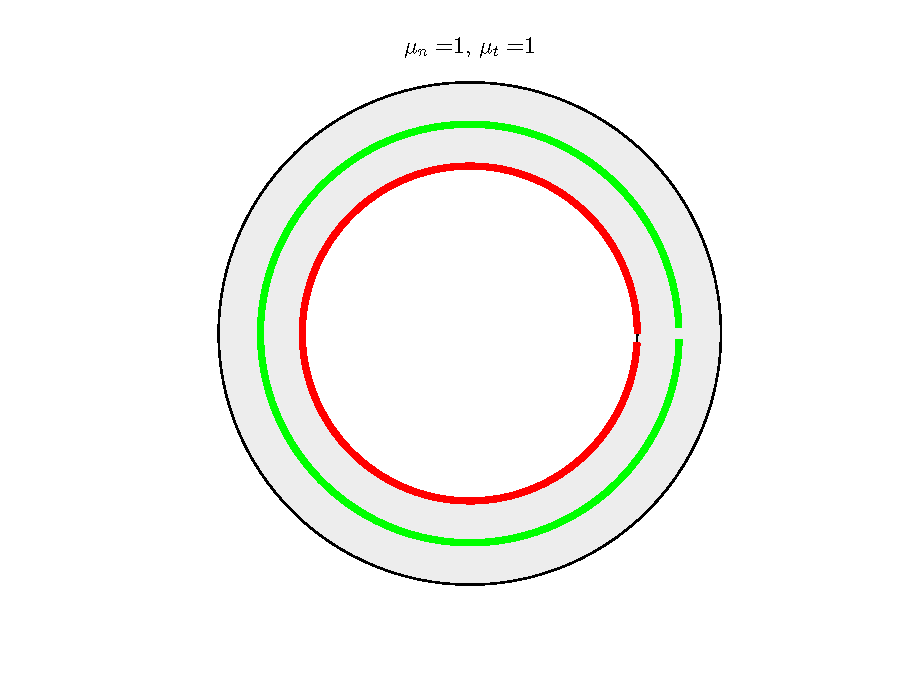
\includegraphics{graficos/circular/trayectoria1}
\begin{tabular}{cc}
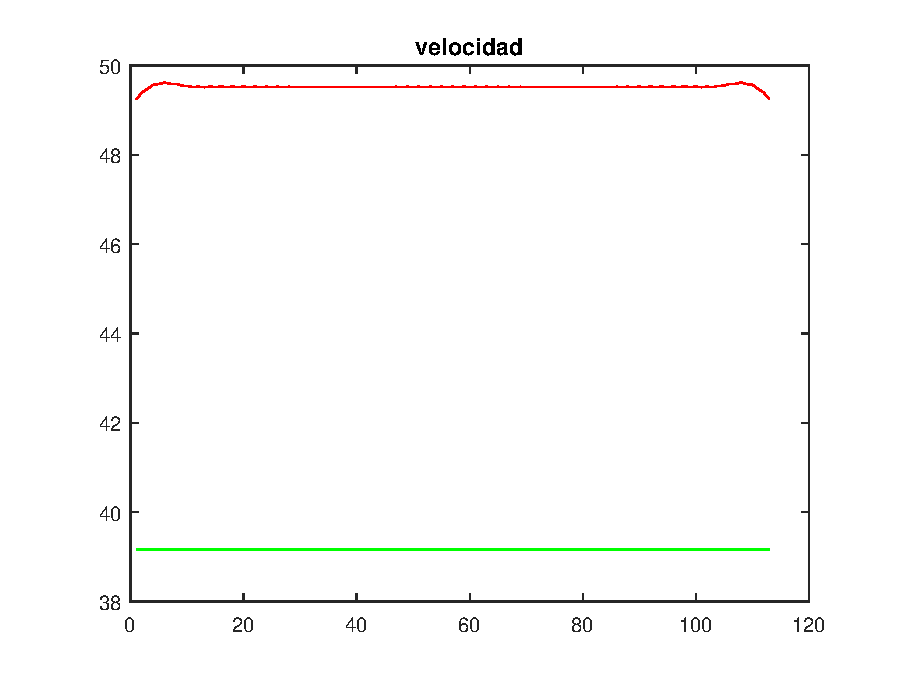
\includegraphics[scale=0.5]{graficos/circular/velocidad1} &
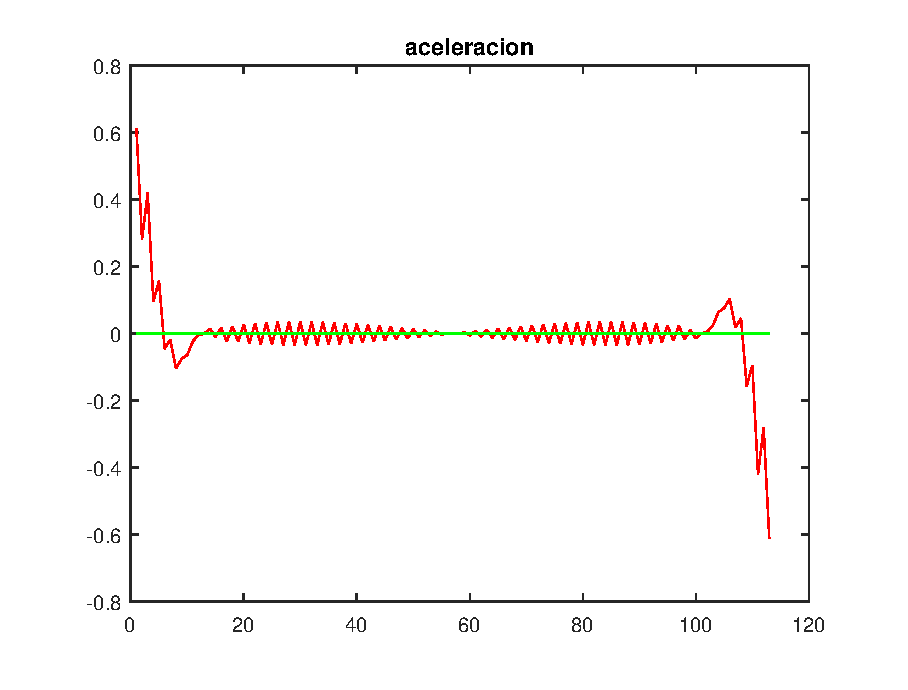
\includegraphics[scale=0.5]{graficos/circular/aceleracion1}
\end{tabular}
\caption{Curvas iniciales en verde y finales en rojo.}
\label{circ1}
\end{figure}

\begin{figure}[h!]
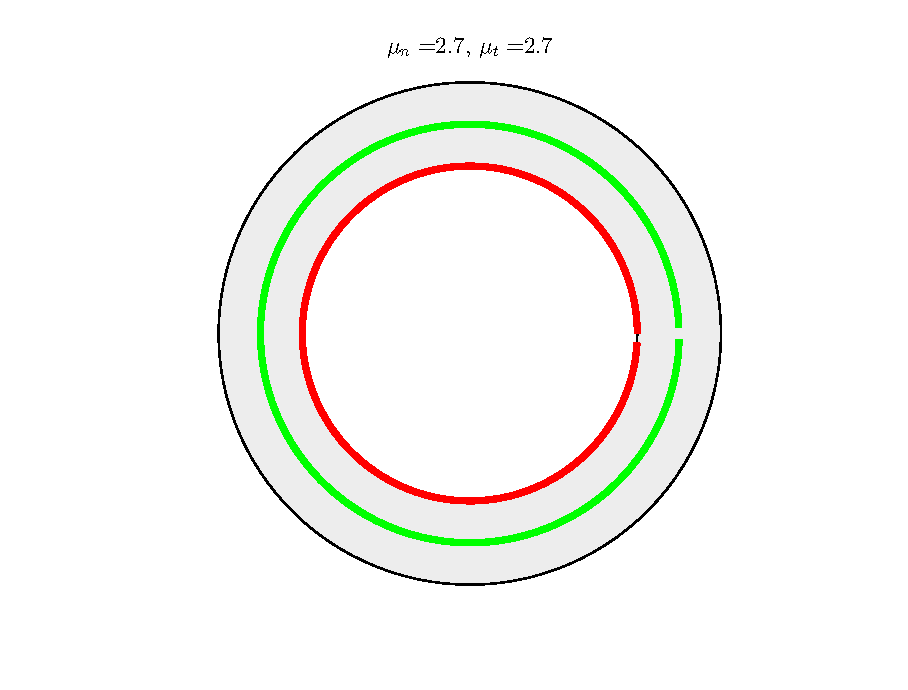
\includegraphics{graficos/circular/trayectoria2}
\begin{tabular}{cc}
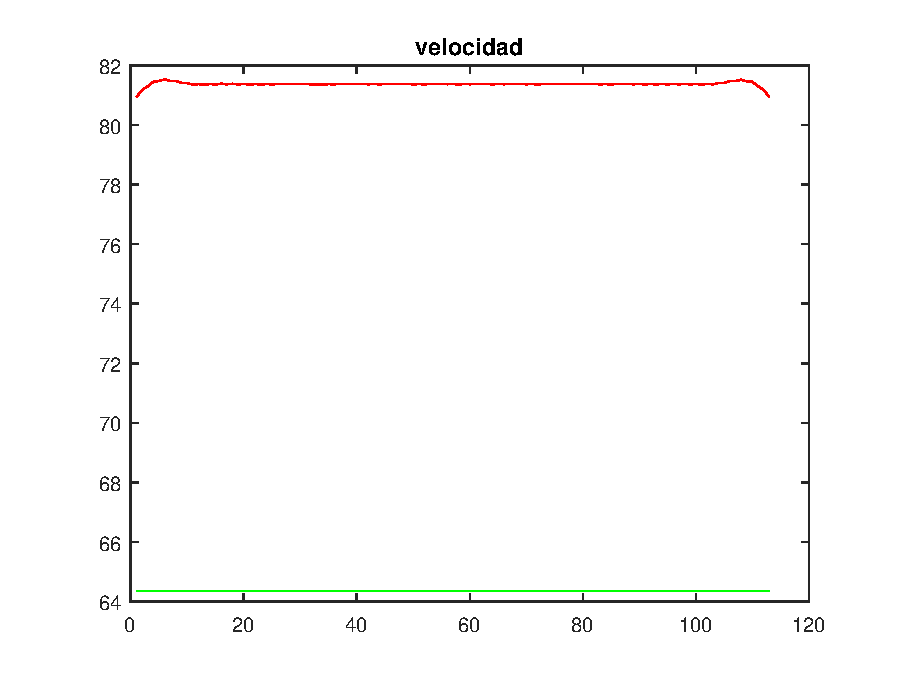
\includegraphics[scale=0.5]{graficos/circular/velocidad2} &
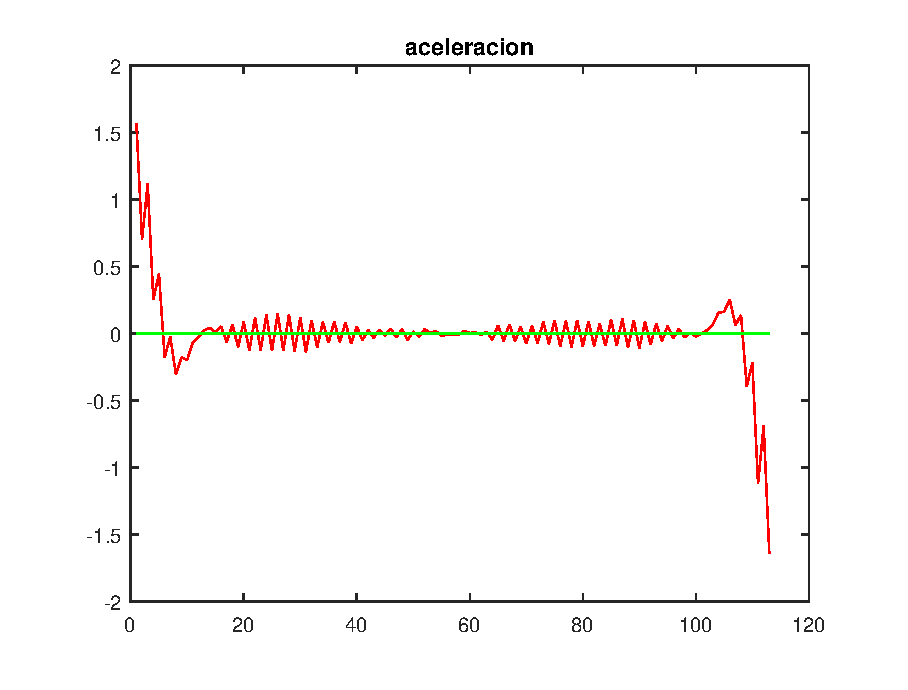
\includegraphics[scale=0.5]{graficos/circular/aceleracion2}
\end{tabular}
\caption{Curvas iniciales en verde y finales en rojo.}
\label{circ2}
\end{figure}

\begin{figure}[h!]
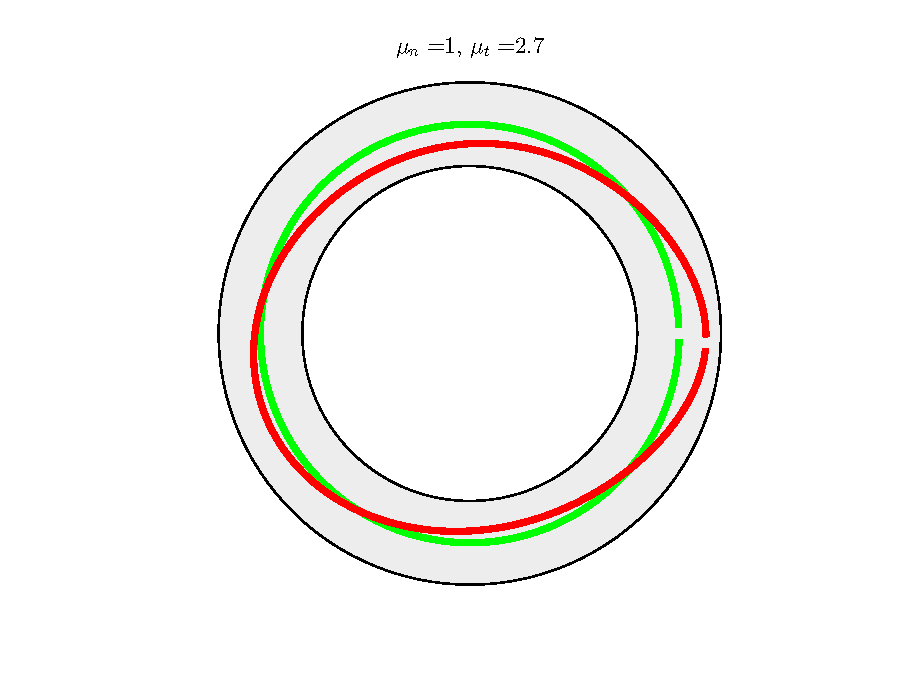
\includegraphics{graficos/circular/trayectoria3}
\begin{tabular}{cc}
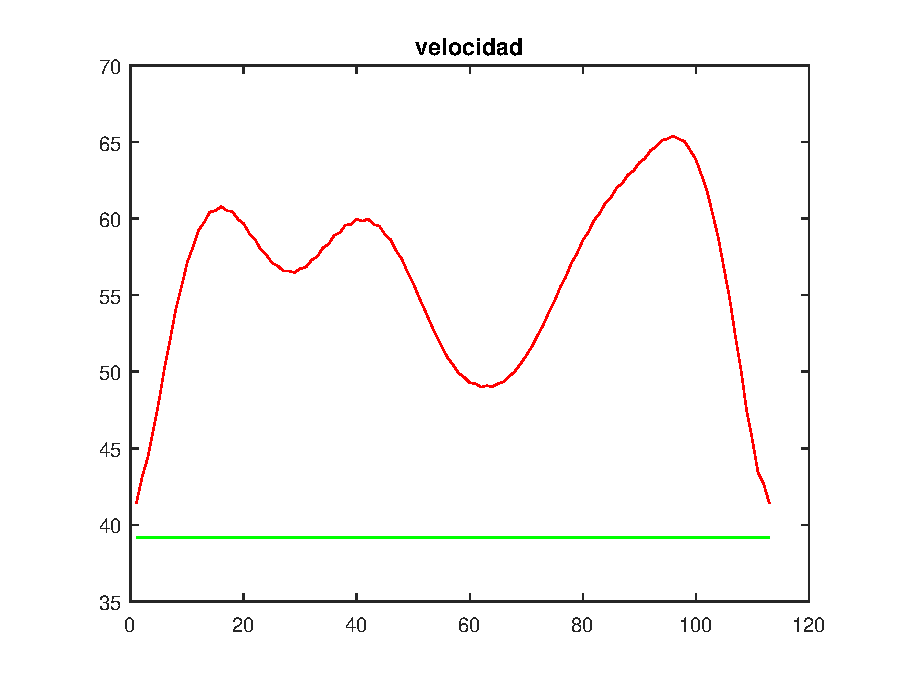
\includegraphics[scale=0.5]{graficos/circular/velocidad3} &
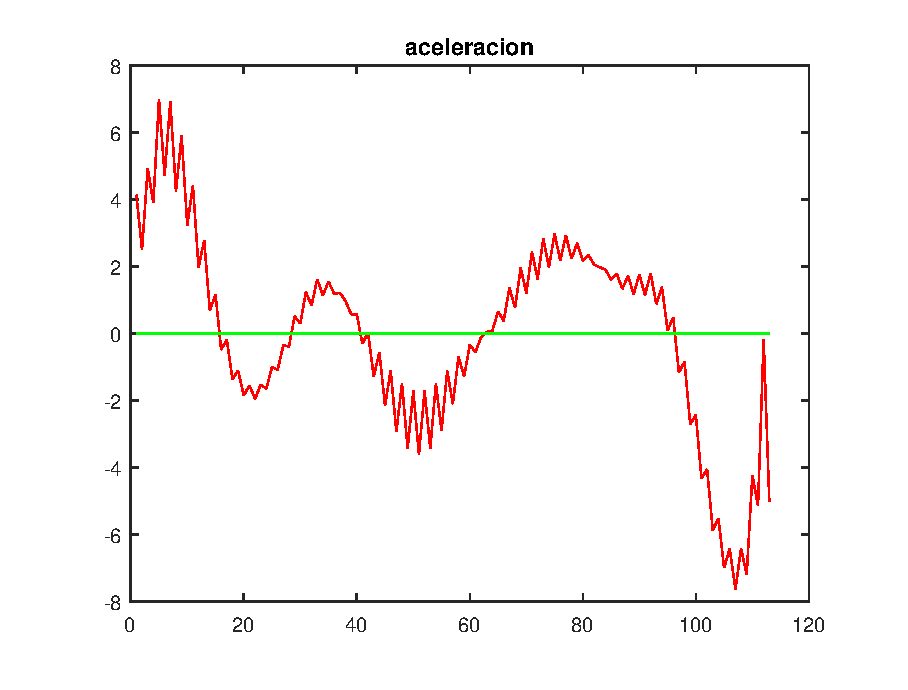
\includegraphics[scale=0.5]{graficos/circular/aceleracion3}
\end{tabular}
\caption{Curvas iniciales en verde y finales en rojo.}
\label{circ3}
\end{figure}

Se puede visualizar que la trayectoria óptima de las Figuras \ref{circ1} y \ref{circ2} es recorrer la calzada interna. Sin embargo la trayectoria de la Figura \ref{circ2} se recorre a mayor velocidad, debido al aumento de las constantes de rozamiento. Es posible inferir, que esto se debe principalmente a que, aumentando el rozamiento normal es más fácil girar a mayor velocidad, ya que el vehículo se adhiere mejor a la pista tomando en la curva. A causa de que la pista es circular, el coeficiente de rozamiento tangencial no tiene demasiada influencia.

Tal vez estos resultados puedan parecer un poco triviales, no obstante, se pueden visualizar trayectorias óptimas distintas en una pista similar en \cite{romeromecanica}. Además, al modificar las constantes de rozamiento el algoritmo puede realizar más iteraciones de las permitidas sin poder encontrar una trayectoria óptima, como puede verse en la Figura \ref{circ3}.


A continuación, se procederá a variar un poco más los circuitos, por ejemplo, cuando tanto la calzada interna como la externa son cuadradas.

\section{Pista cuadrada}
\begin{figure}[h!]
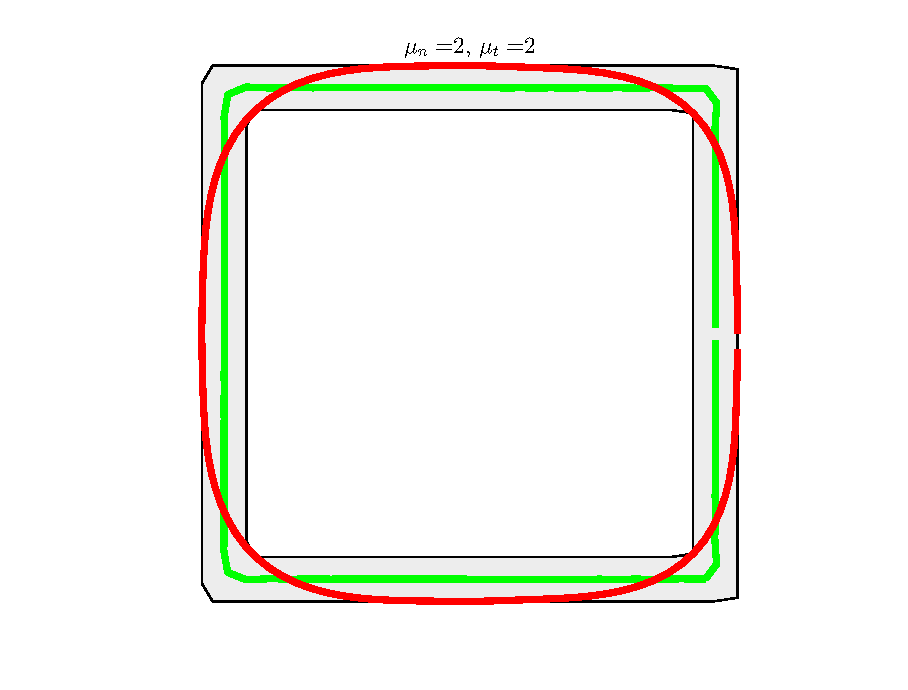
\includegraphics{graficos/cuadrada/trayectoria}
\begin{tabular}{cc}
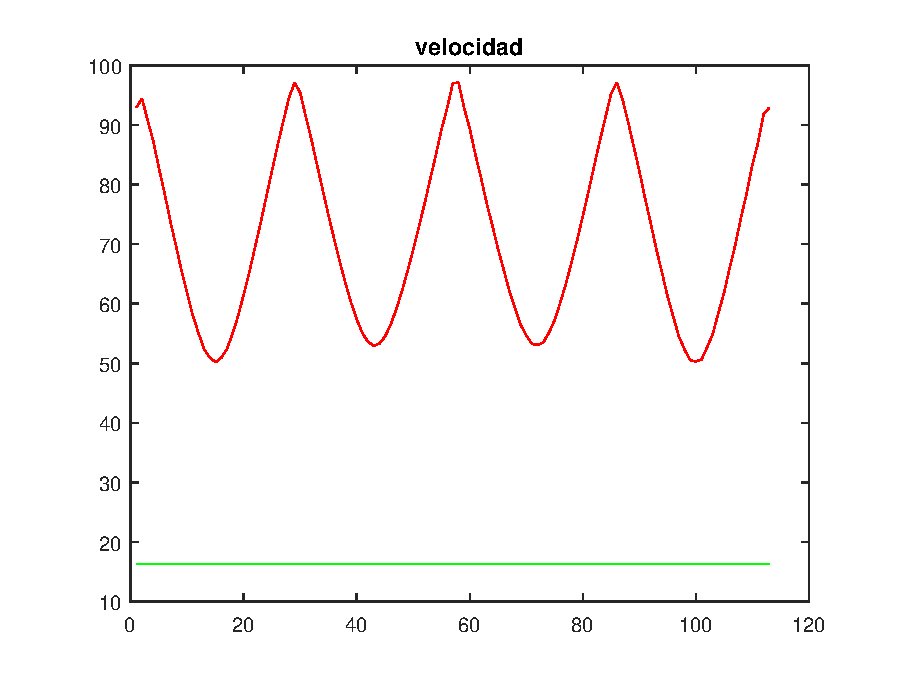
\includegraphics[scale=0.5]{graficos/cuadrada/velocidad} &
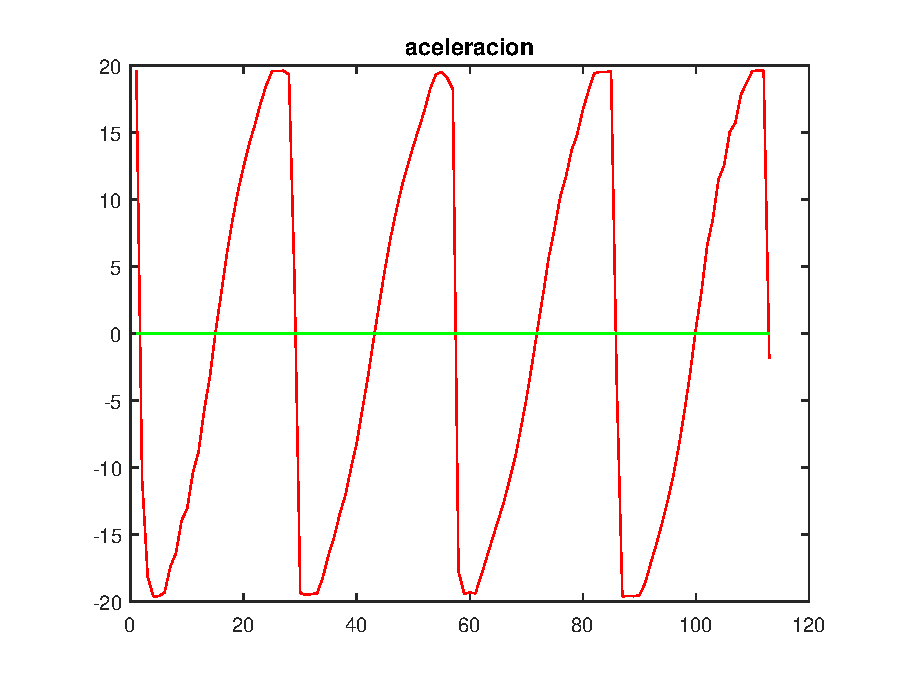
\includegraphics[scale=0.5]{graficos/cuadrada/aceleracion}
\end{tabular}
\caption{Curvas iniciales en verde y finales en rojo.}
\label{cuadrada}
\end{figure}
Se puede observar que la trayectoria óptima en la Figura \ref{cuadrada} es suave y semejante a una circunferencia dentro de los límites de la pista. 

%Se puede observar ahora, que seguir la calzada interna, ya no es la trayectoria óptima, sino, lo optimal es una trayectoria suave (semejante a una circunferencia) que sólo interseca la calzada interna en los vértices de la misma.

\section{Pista irregular}
Finalmente, se utiliza el algoritmo para encontrar las trayectorias óptimas de dos circuitos más complejos, similares a los de pistas de carreras.
\begin{figure}[h!]
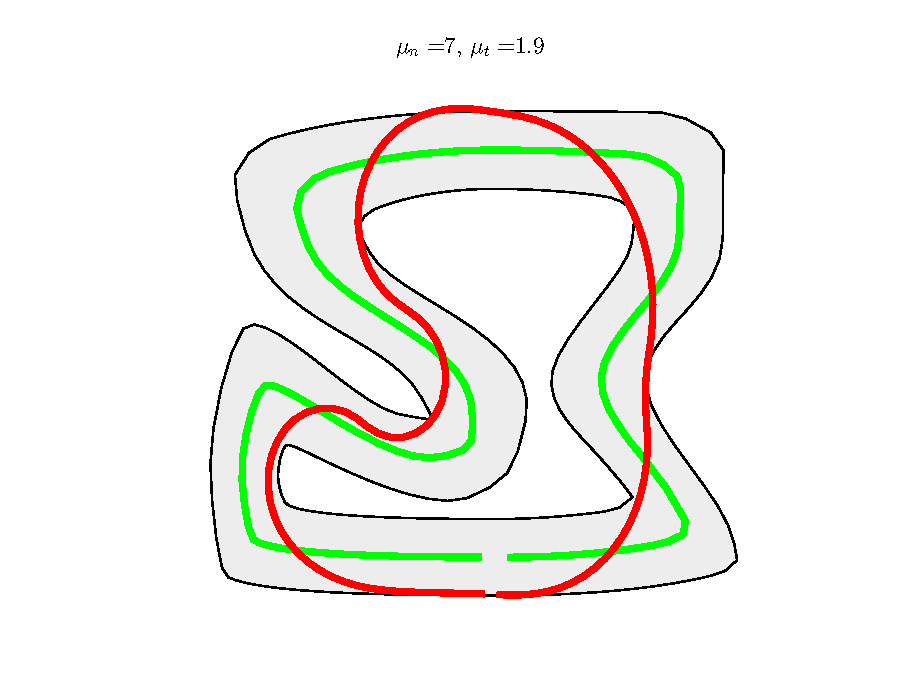
\includegraphics{graficos/irregular/trayectoria}
\begin{tabular}{cc}
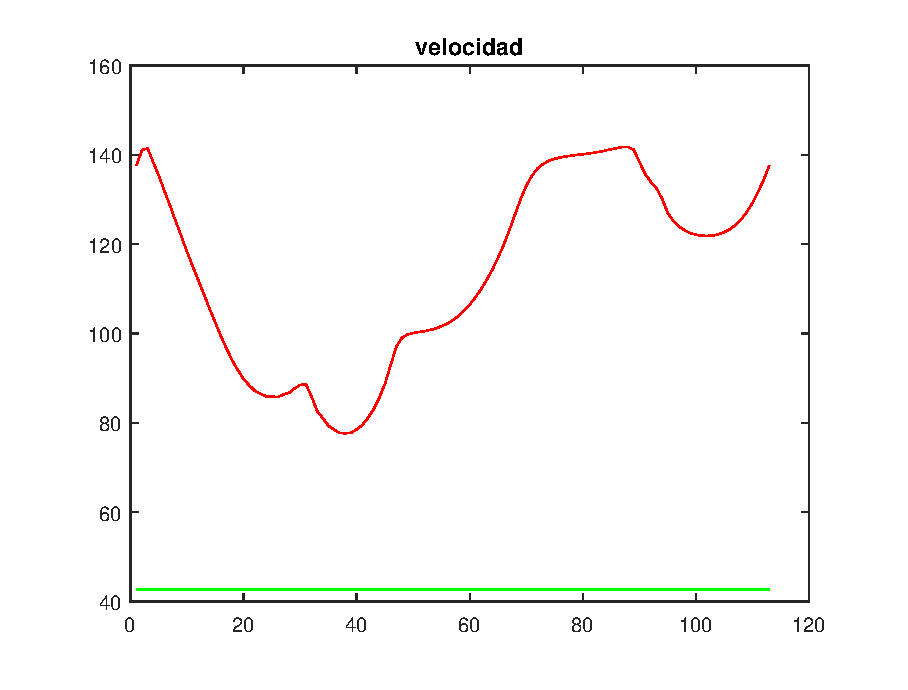
\includegraphics[scale=0.5]{graficos/irregular/velocidad} &
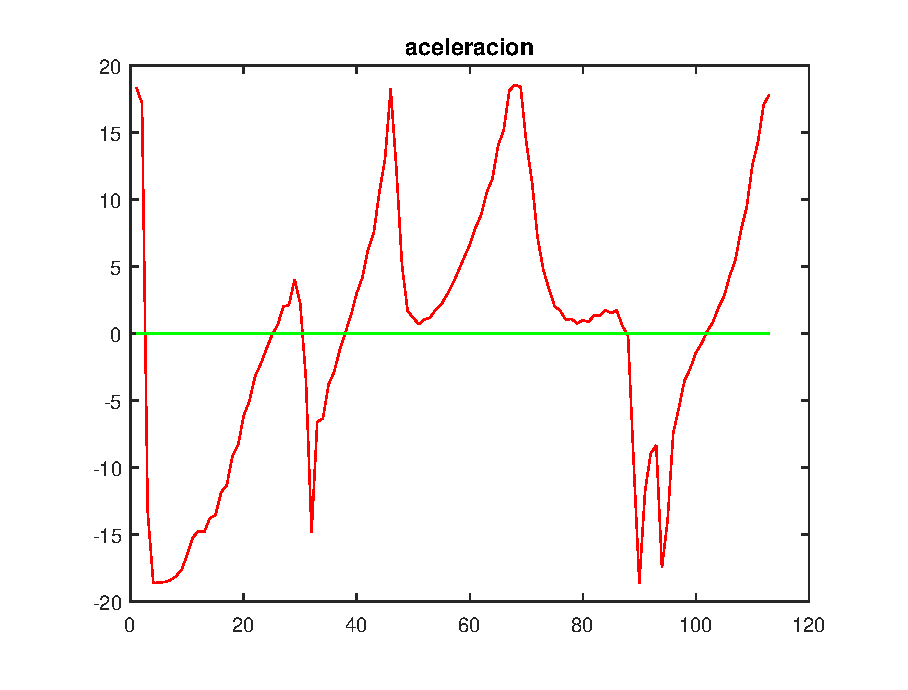
\includegraphics[scale=0.5]{graficos/irregular/aceleracion}
\end{tabular}
\caption{Curvas iniciales en verde y finales en rojo.}
\label{irregular}
\end{figure}

Observando la gráfica de la trayectoria óptima en la Figura \ref{irregular}, es posible ver que la misma intenta mantener cierta suavidad constantemente, de manera que pueda lograr la mayor aceleración posible, teniendo en cuenta la fricción de la pista. Y se obtiene algo similar en la segunda pista (Figura \ref{irregular2}).

Observando todas las trayectorias óptimas anteriores, una manera interesante de describir lo obtenido es que el algoritmo produce una trayectoria dentro de los límites de la pista, que cumple la ecuación de fricción y que tiene \texttt{curvatura constante a trozos}, ya que justamente, a trozos, la trayectoria óptima es recta (curvatura cero), o similar a un círculo (curvatura constante).

Note que además, los picos en las gráficas de velocidad y aceleración son coherentes con la trayectoria en el siguiente sentido: cuando el vehículo toma una curva cerrada, debe disminuir su velocidad y por lo tanto tendrá aceleración negativa, de la misma manera cuando el recorrido próximo es recto, se puede observar un aumento en la velocidad y una aceleración positiva.
\begin{figure}[h!]
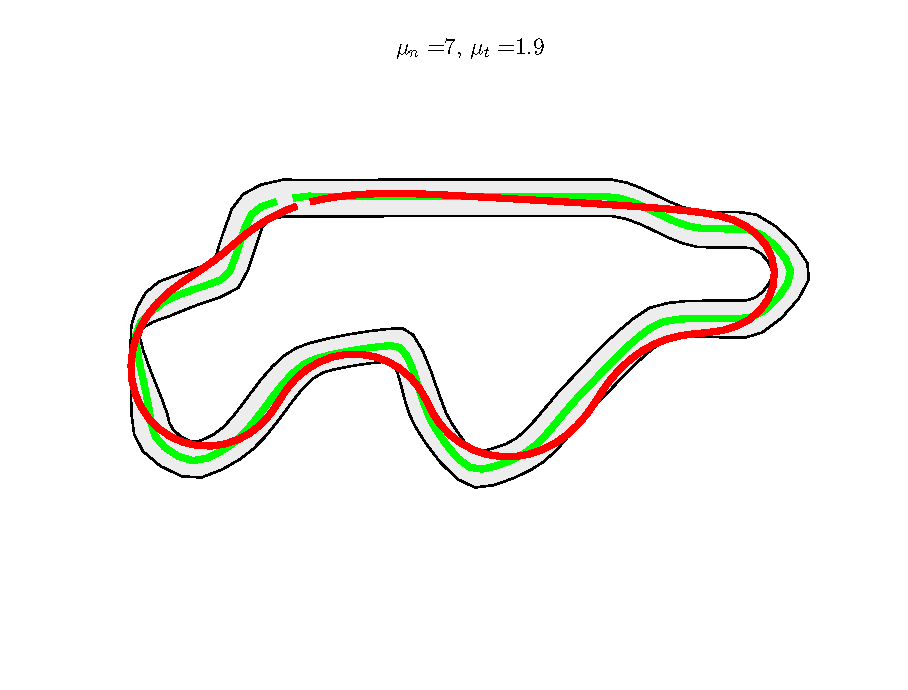
\includegraphics{graficos/irregular/trayectoria2}
\begin{tabular}{cc}
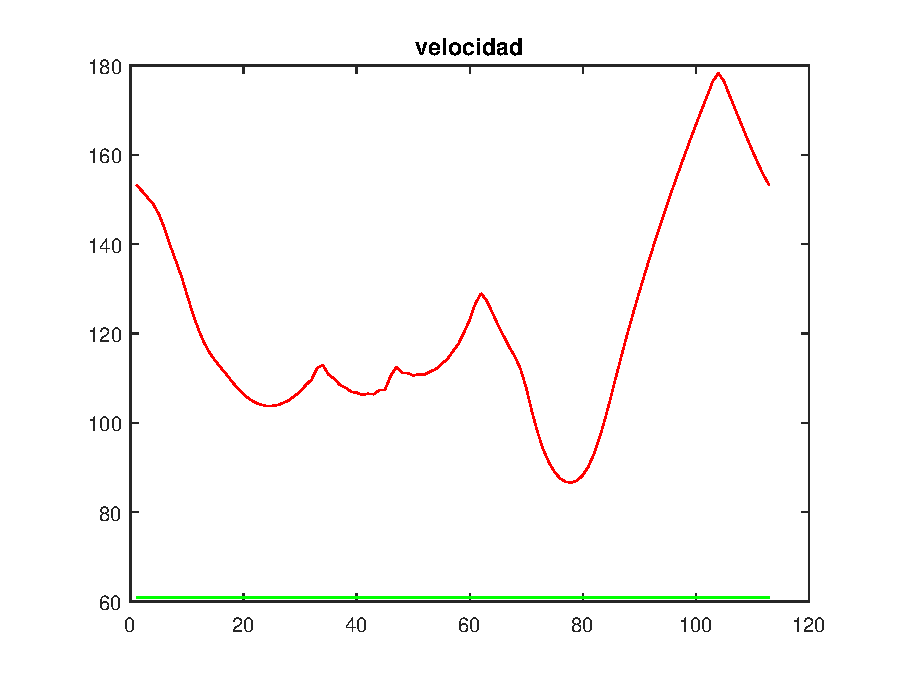
\includegraphics[scale=0.5]{graficos/irregular/velocidad2} &
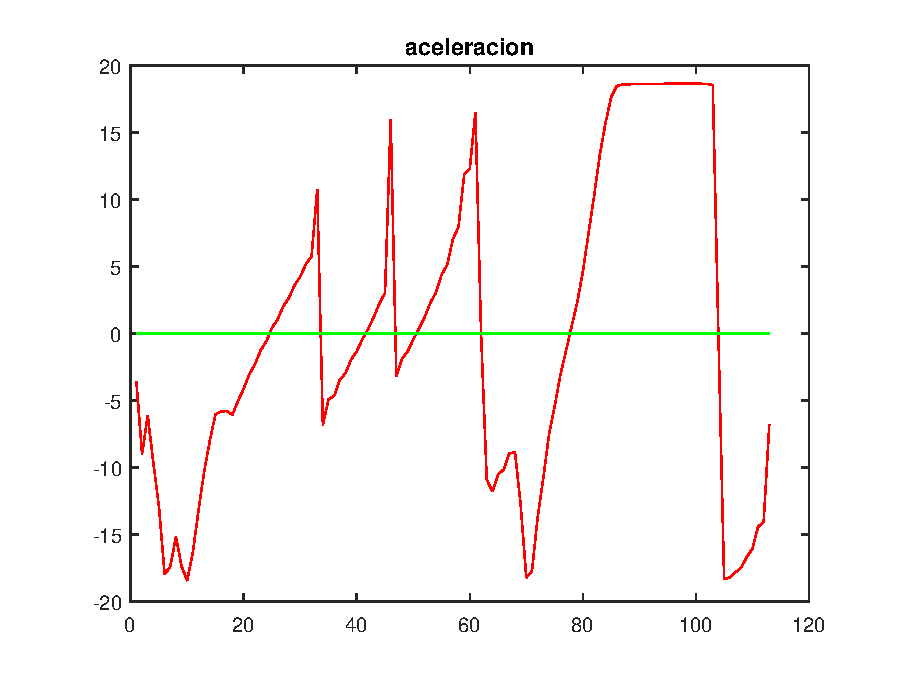
\includegraphics[scale=0.5]{graficos/irregular/aceleracion2}
\end{tabular}
\caption{Curvas iniciales en verde y finales en rojo.}
\label{irregular2}
\end{figure}

\chapter{Conclusión}

De acuerdo a lo realizado en este trabajo, se puede concluir que se logró el objetivo de plantear y resolver el problema de optimización propuesto, es decir, se encontró una manera de obtener una trayectoria óptima, en un circuito cerrado. Además el código programado también provee la aceleración tangencial y la rapidez. También en este trabajo se realizó una introducción a la teoría de existencia de soluciones para problemas de optimización en dimensión infinita y existencia de multiplicadores de Lagrange tanto en dimensión infinita como en dimensión finita, además de una descripción del método computacional SQP, utilizado para resolver el problema de optimización.

El trabajo puede ser utilizado para cualquier circuito de carreras, sólo es necesario dar las coordenadas de las pistas como se puede ver en la Subsección \ref{pistas}. Sin embargo puede tener diversos usos, como por ejemplo optimizar el recorrido en líneas de producción de fábricas, sólo habría que modificar el problema planteando la correspondiente ecuación de restricción de fricción (ya no necesariamente sería una elipse).

El problema de encontrar una trayectoria óptima es muy estudiado, en particular hay trabajos que se concentran en circuitos automovilísticos, tomando en cuenta muchas más restricciones físicas, donde el vehículo ya no es puntual, sino que es un automóvil. Artículos de este tipo pueden observarse por ejemplo en \cite{xiong2010racing,van2015optimal,romeromecanica}. 







\chapter{Apéndice}


\section{Códigos para MATLAB}

\subsection{Principal}\label{main}
\lstinputlisting{codigos/principalB.m}

\subsection{Pistas}\label{pistas}
\subsubsection{Pista circular}
\lstinputlisting{codigos/pista_circular.m}
\subsubsection{Pista cuadrada}
\lstinputlisting{codigos/pista_cuadrada.m}
\subsubsection{Pista irregular 1}
\lstinputlisting{codigos/pista_irregular1.m}
\subsubsection{Pista irregular 2}
\lstinputlisting{codigos/pista_irregular2.m}

\subsection{Función objetivo}\label{fobj}
\lstinputlisting{codigos/fobj_fmincon.m}

\subsection{Función restricción}\label{fres}
\lstinputlisting{codigos/fres_fmincon.m}

\subsection{Gráficos}\label{graficar}
\lstinputlisting{codigos/graficar.m}

%\begin{defi}
% La funcion Lagrangiana aumentada asociada a ($\tilde{P}$) es
% 
% $L_c:\R^n\times\R^m\times\R^r\arr\R$ tal que 
% $$L_c(x,\lambda,\mu)=f(x)+\la\lambda , h(x)\ra %+\frac{c}{2}\|h(x)\|^2+\frac{1}{2c}\sum_{j=1}^r(\mbox{máx}\{0,\mu_j+cg_j(x)\}^2-\mu_j^2)$%$.
%\end{defi}

%\textbf{Método del Lagrangiano aumentado}

%Dado $\lambda^0, \mu^0, c_0^0>0$; genero $\{x^k\}, \{\lambda^k\}, \{\mu^k\},\{c_k\}$

%PASO 1. Tomo $x^{k+1}$ solución de 
%\[
%\left\{\begin{array}{rl}
%\displaystyle \mathop{\mathrm{minimizar}}_{x\in\Omega} & \displaystyle %L_{c_k}(x,\lambda^k, \mu^k)
%\end{array}\right.
%\].
%PASO 2. Defino $$\lambda^{k+1}= \lambda^k + c_k h(x^{k+1})$$ y
%$$\mu^{k+1}=\mbox{máx}\{0,\mu^k+c_k g(x^{k+1})\}$$.

%ASO 3. Tomo $c_{k+1}\geq c_k$.

%\begin{prop}
 %Asuma f,g y h continuas. $\Omega\subset\R^n$ cerrado y $X$ no vacío. Consideremos las %sucesiones $\{x^k\}, \{\lambda^k\},\{\mu^k\} y \{c_k\}$ generadas por el método del %Lagrangiano aumentado tal que $x^{k+1}$ es solución global, $\{\lambda^k\},\{\mu^k\}$ %acotadas y $c_k\arr\infty$ Entonces todo punto límite de $\{x^k\}$ es un mínimo global %de $\tilde{P}$.
%\end{prop}


















%\nocite{*}
\bibliographystyle{abbrv}%{plain}
\bibliography{bibliografia}  

% \newpage
% \thispagestyle{empty}
% %\chapter*{}
% \vspace{5cm}
% Los abajo firmantes, miembros del Tribunal de Evaluación de tesis, damos Fe
% que el presente ejemplar impreso, se corresponde con el aprobado por éste
% Tribunal.

% \vspace{5cm}

% \begin{tabular}{p{0.3\textwidth} p{0.3\textwidth} p{0.3\textwidth}}
% $\overline{\mbox{Damián Fernández}}$ & $\overline{\mbox{Elvio Pilotta}}$& $\overline{\mbox{Andrés Barrea}}$ 
% \end{tabular}


\end{document}